\documentclass{usydthesis}

% Configuration

\def\degree{Bachelor of Information Technology (Honours)}
\def\department{School of Information Technologies}

\title{{\bf\Huge Data Mining Methods for Predicting Length of Hospital Stay}}
\author{Tianyu Pu}
\def\sid{310182212}
\def\supervisor{Associate Professor Irena Koprinska}
%\def\assocsupervisor{Comment this line to remove assoc supervisor}

%%%%%%%%%%%%
% Packages

\usepackage{alltt}
\usepackage{amsfonts}
\usepackage{amsthm}
\usepackage{booktabs}
\usepackage[colorlinks=true,citecolor=blue,linkcolor=blue,filecolor=blue,urlcolor=blue,pdfborder={0 0 0}]{hyperref}
\usepackage[all]{hypcap}
\usepackage[utf8]{inputenc}
\usepackage{listings}
\usepackage{longtable}
\usepackage{multicol}
\usepackage{multirow}
\usepackage{pbox}
\usepackage{pdflscape}
\usepackage{pgf}
\usepackage{pifont}
\usepackage{qtree}
\usepackage[english,rounding]{rccol}
\usepackage{rotating}
\usepackage{setspace}
%\usepackage{subfigure}
\usepackage{style/bib}
\usepackage{subcaption}
\usepackage{tabularx}
\usepackage{tipa}
\usepackage{verbatim}
\usepackage{wrapfig}
\usepackage{xcolor}
\usepackage{xspace}

\rcDecimalSignOutput{.} % rccol

\newenvironment{sidewaystablepage}{\begin{landscape}\begin{table}}{\end{table}\end{landscape}}

\def\subsectionautorefname{Section}
\def\subtableautorefname{Table}
\def\subfigureautorefname{Figure}
\def\chapterautorefname{Chapter}

\newcommand{\tick}{\ding{51}}
\newcommand{\cross}{\ding{53}}

\newcommand{\todo}[1]{{\color{red} #1}}
\newcommand{\sent}[1]{{\color{blue}\texttt{#1}\xspace}}

\newcommand{\scell}[2][c]{%
  \begin{tabular}[#1]{@{}c@{}}#2\end{tabular}}

\definecolor{mygreen}{rgb}{0, 0.6, 0}
\definecolor{mygray}{rgb}{0.5, 0.5, 0.5}
\definecolor{mymauve}{rgb}{0.58, 0, 0.82}

%%%%%%%%%%%%
% Maths functions
\def\O{\mbox{O}}

%%%%%%%%%%%%
% Setup

%   Page size:
\oddsidemargin=0cm	% really 1in
\evensidemargin=0cm
\textwidth=6.2677165in

% initial page numbers:  i, ii, iii, ...
\renewcommand{\thepage}{\roman{page}}

\DeclareGraphicsExtensions{.png}
%\input{morenames.tex}

%%%%%%%%%%%%
% Start

\begin{document}

%%%%%%%%%%%%
% Title page
\maketitle

\setstretch{1.5}

% intro pages
\cleardoublepage
\phantomsection
\input{plagiarism/plagiarism.tex}
\cleardoublepage
\phantomsection
\chapter*{Abstract}

Predicting the length of hospital stay for injured patients involves making a
judgement about how long they need to be hospitalised, so that doctors and
hospital staff can plan the appropriate course of treatment for the patient
to ensure they recover in the quickest possible time. This also ensures the
most efficient use of limited hospital resources. However, previous studies
have used a limited number of statistical techniques such as logistic
regression in order to predict the length of stay. Also, they have used only
manual feature selection and have not investigated the effect of automatic
feature selection on classifier performance.

Our work systematically evaluates and compares the performance of a number of
state-of-the-art classification algorithms and feature selection methods,
and also assesses the effect of feature discretisation for all combinations
of classifiers and feature selectors. Our evaluation were conducted on two
datasets, one from a trauma ward in a major Sydney hospital and another one
from a general hospital in Portugal. We propose a new classification algorithm
called Ranked Distance Nearest Neighbor that considers the
relative importance of each feature when determining the nearest neighbours.

For the trauma dataset, we were able to achieve an accuracy of 77.81\% with
1-nearest neighbour and an area under the curve of 0.846 with logistic
regression. This represents an improvement of 2.75\% and 0.034 respectively
over the previous best result on the same dataset. For the
general hospital dataset, the best results were 98.23\% accuracy with a
decision tree and 0.994 area under the curve with logistic regression,
support vector machine and K*. We also show that our proposed Ranked
Distance Nearest Neighbour improves accuracy and area under the curve over
traditional nearest neighbour algorithms. We comprehensively discuss
the results and suggest new directions for future studies.

\cleardoublepage
\phantomsection
\chapter*{Acknowledgements}

I would like to thank my supervisor, Dr Irena Koprinska, for her unwavering
support throughout the year. Irena, thank you for always being willing to
listen, and for raising points that inspired me to pursue new directions in
my research.

I would also like to thank Dr Michael Dinh from the Royal Prince Alfred
Hospital, without whom the research in this thesis would not have been
possible. Thank you for providing access to the data we needed for this study,
and for patiently answering all my questions about the data set and your
previous experiments.

Thank you also to Professor Paulo Cortez from the University of Minho in
Portugal for providing an extensive, independent data set from all the way
across the world.

Thank you to all of my friends, in particular Daniel Buckmaster, Stephen
Caraher and Christine Au Yeung, for the selfless encouragement, help and good
times which have made this year-long journey possible.

And, last but not least -- to my parents Caixiu and Ning, and
my sister Lily -- thank you for tirelessly supporting me throughout this year,
especially towards the deadline. This would not have been possible without all
of you.


% tables
\cleardoublepage
\setcounter{tocdepth}{2}
\tableofcontents

{\makeatletter
\renewcommand*\numberline[1]{\hb@xt@\@tempdima{#1 \hfil}\hspace*{1em}}
\makeatother
\listoffigures
\listoftables
\cleardoublepage
}

%%%%%%%%%%%%
% Chapters
\setcounter{page}{1}
\setcounter{chapter}{0}

% main page numbers:  1, 2, 3, ...
\renewcommand{\thepage}{\arabic{page}}	
\setupParagraphs

\chapter{Introduction}

\section{Background}
Suppose that we have a (perhaps large) data set. It could consist of
demographic data taken from a census, details of transactions in a shopping
centre, or simply a collection of text documents. The term used to describe
the methods of analysis used to find unknown relationships and summarise
information in these data sets is \textit{data mining} \citep{Hand2001}.
Broadly speaking,
data mining can be broken down into five areas (or \textit{tasks}) depending
on the aims of the person analysing the data:

\begin{enumerate}
\item Exploratory data analysis (EDA), which consists of simply exploring some
given data set without any particular goal or ideas of what to look for.
Methods in EDA usually involve interaction and visualisation, but this can
become difficult if there are too many data points;
\item Descriptive modelling, as its name suggests, seeks to describe the data
or the processes that generate it. The major areas here are clustering (finding
partitions of the data) and density estimation (finding the probability
distribution of the data);
\item Predictive modelling aims to create models that will allow the value of
some desired quantity or metric to be predicted based on some known or observed
values in the data set. The two major sub-areas of predictive modelling are
\textit{classification} and \textit{regression}, distinguished only by the
nature of the quantity we want to predict. If we want to predict whether
something belongs in a category, such as the disease of a patient, then we
are dealing with classification; otherwise, if we wish to predict a numeric
quantity, such as the value of the stock market at some future date, then
it is a regression problem;
\item Pattern and rule discovery, which covers anomaly detection (finding data
points which do not fit an expected trend, like detecting credit card fraud)
and association rule learning (discovering relationships between various items
in transaction databases, such as the food items purchased frequently together
in a supermarket);
\item Content retrieval, where the user wishes to find patterns in a data set
that are similar to the one he or she specifies. Search engines are a familiar
application of this area of data mining.
\end{enumerate}

The technical methods of data mining are drawn substantially from a field of
computer science known as \textit{machine learning}, which is dedicated to the
study of systems that can learn structural descriptions from data examples.
In this thesis we will focus on the task of predictive modelling, also
known as \textit{supervised learning} in the field of machine learning.
Specifically,
our problem will be one of classification. We will introduce the necessary
terminology in the next section as we describe the problem, as well as
throughout this thesis as necessary.

\section{Problem Statement}
Consider a data set of patients admitted to the trauma ward of a hospital.
This data set looks like a very large table: there are many columns, each one
describing some aspect of a patient (for example, age); there are also many
rows, each corresponding to a particular patient that was admitted. We will
refer to the columns as \textit{features} or \textit{attributes}, so-named
because they describe some particular aspect of the rows, which are often
called \textit{instances}, \textit{samples}, or \textit{training examples}.
Concretely, as an example, our data set could contain
two features (age and gender) for five patients: as a table, this means that
we have two columns, one for age and another for gender, with five rows
containing the age and gender data for each patient. Attributes can be numeric
(such as age) and potentially take on an infinite number of different values,
or categorical (such as gender) and can only have one of a limited, pre-defined
list of values.

In a general supervised learning problem, we wish to predict a value for some
desired quantity given some values for the attributes. The relationship between
the features and the desired quantity can be \textit{learned} from using data
that contains known values for the quantity that we wish to predict: this is
what makes the problem \textit{supervised}.
Our problem is a binary \textit{classification} task in which we
predict one of two possible categories for a patient: a length of stay (LOS) of
less than or equal to 2 days, or a LOS of greater than 2 days. These outcomes
are also called \textit{classes} or \textit{class labels}.

To do this, we use our data set of trauma patients with \textit{known}
values for the LOS and apply various \textit{learning} or
\textit{classification algorithms} to deduce
a relationship between the features and the LOS. Once the learning algorithm
or \textit{classifier}
has ``learned'' this relationship, it is then able to predict the class of
any patient given a set of features describing him or her.
Note that the LOS is simply another attribute of our data set; however, because
it is the quantity that we are interested in predicting, it is also called the
\textit{target}, \textit{outcome}, or \textit{class}.

\section{Motivation}
The LOS is an important measure of resource utilisation in hospitals around
the world \citep{Ng2006},
and many studies have been carried out to investigate whether the
LOS of a patient in various medical domains -- after surgery, burns, or
intensive care treatment to name a few -- can be predicted accurately.
Regardless of the
specifics of the problem, accurate LOS prediction results in better planning
and management of limited resources such as staff, equipment and medical
supplies. This is particularly critical as hospitals often face the problem
of limited funding \citep{Walczak2003}.
As we will see in the next chapter, there has been limited
application of a variety of data mining techniques to predict the LOS in
various medical domains, including trauma. Our work will aim to bridge this
gap by providing insights on the application of a wide range of data mining
techniques to LOS prediction.

\section{Contributions}
The work presented in this thesis aims to address several gaps in the current
research into LOS prediction, by building upon the work of Dinh et al.
\citep{Dinh2013a}. Our contributions can be summarised as follows:

\begin{enumerate}
\item We systematically evaluated the performance of a catalogue of eleven
classification algorithms and five feature selection methods for predicting the
LOS of trauma patients. Three of the classifiers and four of the feature
selection methods have not been applied in LOS prediction to date, and only
one has been applied in our medical domain. 

\item We assessed the effect of feature discretisation on classifier
performance. This has not been studied in previous work.

\item We proposed a new algorithm, Ranked Distance Nearest Neighbour, and
showed that it performed better than the standard nearest neighbour algorithm
in certain situations.

\item We conducted our evaluations on two independent data sets from different
medical domains: one from a trauma ward in a major Sydney hospital and the other
from a general hospital in Portugal. The collection, processing and
understanding of the data involved collaboration with medical experts (Dr
Michael Dinh from the Royal Prince Alfred Hospital in Sydney) and researchers
from Portugal (Associate Professor Paulo Cortez from the University of Minho).
Not only is the evaluation of a second data set in one work uncommon in the
literature, the inclusion of more than one data set allowed us to draw
additional insights about the classifiers and feature selections we used
which would not have been possible with only one set of data. 

\item We comprehensively analysed and discussed various aspects of the results
(such as comparison across classification algorithms, feature selection
methods, performance measures, datasets and discretisation). Our results showed
an improvement over the best result on the same datasets.
\end{enumerate}

\section{Thesis Outline}
This thesis is structured as follows. Chapter \ref{chap:litreview} introduces
the major methods in supervised learning as used in past work on LOS
prediction. We explore the major algorithms, summarise the current state of
research, and identify where our work fits within this area.

Chapters \ref{chap:classification}, \ref{chap:preprocess} and
\ref{chap:selection} describe in detail the classification algorithms, and
feature preprocessing and selection methods used in our work. This leads into
the process of our evaluation, which is detailed in Chapter
\ref{chap:evaluation}.

Our findings are presented and discussed in Chapter \ref{chap:results}.
We conclude in Chapter \ref{chap:conclusion}, with indications for future
work in this area.

\chapter{Predicting the LOS: A Review} \label{chap:litreview}

\section{Introduction}
Hospitals often have limited funding, and therefore managing and utilising
their resources efficiently has always been a priority \cite{Walczak2003}.
One key measurement of hospital activity, health care utilisation, and hospital
cost is the patient length of stay \citep{Omachonu2004,Ng2006}. The length of
stay has been used in a wide variety of medical domains, such as burns
 \citep{Yang2010}, intensive
care \citep{Tu1993,Harper2005,Perez2006,Dybowski1996},
psychiatry \citep{Lowell1997}, and acute pancreatitis \citep{Pofahl1998}, in
order to assist hospitals in allocating beds and other patient management
resources as efficiently as possible. However, given the many different
conditions that hospitals manage, the length of stay of a patient is
not easy to predict \citep{Walczak2003}, especially upon a patient's admission.
Many methods have been explored in the literature, from the realm of statistics
to techniques in data mining, and they have been explored for many different
medical domains.

One of the more well-understood and widely used statistical methods for
predicting the length of stay is \textit{logistic regression} \citep{Tu1996}.
Logistic regression models are straightforward to construct and use via the
help of statistical software packages such as
SAS\footnote{SAS Institute, Cary, NC, USA}, and
also make the contribution of each independent variable to the final
prediction explicit. Thus they is easy to interpret when compared to more
``black box'' approaches such as artificial neural networks \citep{Adams2012}.
A wide variety of other statistical approaches have been proposed, notably:
various scoring systems from univariate analysis \citep{Adams2012,Lavoie2005},
linear regression \citep{Yang2010}, exponential models \citep{Clark2007},
survival analysis \citep{Vasilakis2005}, and Markov
models \citep{Perez2006,Jain1989,Kapadia2000}.

Out of the development of the various statistically-motivated models, data
mining techniques, particularly artificial neural networks,
began to become more widely adopted following a number of
early applications to length of stay prediction in intensive
care \citep{Tu1993,Dybowski1996}, in addition to disease diagnosis and mortality
prediction \citep{Silva2006}. Artificial neural networks are able to detect
complex and non-linear relationships between input and output variables and can
be developed using many different techniques. Much work has been done in using
neural networks to predict patient length of stay in various medical conditions
such as acute pancreatitis \citep{Walczak2003}, gastroenteritis \citep{Ng2006},
surgical intensive care \citep{Buchman1994,Tu1993} and
psychiatry \citep{Lowell1997}. Other data mining techniques have also been
applied, such as support vector machines and tree-based
methods \citep{Harper2005}.

Given the benefits to the hospital of accurate length of stay prediction,
this research aims to build upon improving length of stay prediction for trauma
patients by utilising state-of-the-art data mining techniques. Being able to
predict the length of stay for trauma patients is especially crucial because of
the scarcity of patient care resource in this area \citep{Yang2010}.
Additionally,
despite the wealth of research into length of stay prediction in various
medical domains, there has been little work done in generalising models from
one domain to another, or to predict a combination of outcomes (not only
length of stay, but mortality, or rehabilitation requirement). Being able to
do this would mean that hospital staff are better equipped to handle patient
cases and prepare for possible critical outcomes well in advance, resulting
in time and resources saved for both hospital and patient.

This literature review is structured as follows. We will first describe the
various statistical modelling techniques for predicting length of stay that
have been used in the literature, followed by a review of the data mining
techniques and how they compare in terms of accurately being able to predict
patient length of stay. The review will conclude with a summary and a
discussion on the gaps in the literature and how this work intends to address
those gaps.

\section{Statistical Methods}
\subsection{Regression}
As we stated earlier, logistic regression is a commonly-used modelling
technique for prediction in the medical domain \citep{Tu1996}, and especially
in the trauma data analysis \citep{Gabbe2005}. A series of
predictor (independent) variables (or features) determine the probability of a
particular outcome by an equation of the form
\begin{equation}
\mathrm{log}\left(\frac{p}{1-p}\right) = \beta_0 + \beta_1X_1 + \beta_2X_2 + \dots + \beta_nX_n
\end{equation}
where $p$ is the probability of the desired outcome, $\beta_i$ are coefficients
associated with each variable, and $X_i$ are the values of the independent
variables \citep{Hosmer1989}. A stepwise selection algorithm is often used to
choose which variables to include in the model out of all available variables:
different algorithms produce different models which are then compared against
one another to find the best model. Usually, a standard maximum-likelihood
procedure is followed in order to obtain values for the $\beta_i$'s, and models
can be tested using measures such as the area under the receiver operating
characteristic (ROC) curve (AUC) and the Hosmer-Lemeshow statistic.

This is the method that Gabbe et al. used in their study to identify factors
that contributed to trauma patient length of stay and use these factors to
subsequently predict length of stay \citep{Gabbe2005}. The prediction problem
they proposed was essentially a binary classification problem, to which
logistic regression is well suited \citep{Tu1996}: will length of stay be
\textit{less than 5 days}, or \textit{equal to 5 days}? They used a
\textit{backward} stepwise selection algorithm, whereby all available variables
were initially included in the model and then progressively eliminated if their
likelihood ratio (LR) test $P$-value was $>0.15$. Features could only be
re-included if $P<0.05$. For length of stay
prediction, this left them with 9 features out of the 15 that they originally
included. To validate their model, they used a data set collected from an
independent source which had slightly different statistical characteristics for
the various features and outcomes. Their length of stay prediction model was
found to have 95\% sensitivity and 24\% specificity, with an area under the ROC
curve (AUC) of 0.62. This indicates that the model is not able to discriminate
length of stay cases of less than 5 days and equal to 5 days (i.e., the two
desired outcomes) very well, and only does
slightly better than simply random guessing (which has AUC 0.50).

In a similar study, Dinh et al. sought to predict whether or not trauma
patients could be predicted to stay in hospital \textit{less than 2 days} or
\textit{greater than 2 days} \citep{Dinh2013a}.
They also used a logistic regression model and
selected their features using a stepwise selection algorithm with the same
$P$-value threshold (0.05). Even though we cannot compare their result to that
of Gabbe et al. above because the models were tested on completely different
data sets, it is interesting to note that the model obtained by Dinh et al.
had an AUC of 0.83 after bootstrap cross-validation\footnote{A technique of
sampling a single data set with replacement: e.g. given a set of 100 records,
we can create a bootstrap sample that also contains 100 records which contains
records from the original set drawn at random with replacement. This means that
some records may appear in the bootstrap sample more than once and some may not
appear at all. In the work of Dinh et al., they performed this sampling 500
times (thereby creating 500 data sets) to evaluate the performance of their
model}. This indicates that the model had much better discrimination between
the two values for the outcome. Again, while we cannot directly compare, the
better performance could be due to the availability of more relevant features
to the outcome: Gabbe et al. included very few features specific to trauma
such as place of injury and mechanism of injury \citep{Gabbe2005} whereas Dinh
et al. also had variables for certain kinds of injuries (such as if it was
penetrating), specific body regions that were affected, and whether operations
were required. Given the nature of the length of stay, it would seem that Dinh
et al. derived a model that had included features with more explanatory power
on the outcome, thereby obtaining better results. This idea is consistent with
Buchman et al., who used logistic regression to predict the probability of a
patient in a surgical intensive care unit staying greater than a
week \citep{Buchman1994}.

While logistic regression is simple to use and its results straightforward
to interpret, the above approaches have described a coarse two-class prediction
problem, namely that of predicting the length of stay less than or greater than
a certain threshold. A number of \textit{linear} regression models have been
explored in the literature that examine the task of predicting length of stay
as a continuous quantity.

The key difference between linear and logistic regression is the nature of the
dependent variable: in linear regression it is treated as continuous (i.e., it
can take on any value), whereas in logistic regression it is a dichotomy of
only two values. The works discussed above only considered predicting the
length of stay as two possible outcomes, less than or greater than a particular
threshold of time. We have already stressed the importance of accurate length
of stay prediction for hospitals, and therefore it makes sense that attempting
to predict length of stay as a continous variable could give us more accurate
and useful insight and facilitate better resource allocation.

Yang et al. \citep{Yang2010} used a linear regression model as the baseline for
performance benchmarking when trying to predict the length of stay of burn
patients. Interestingly, unlike the logistic regression models discussed above,
they did not perform any feature selection when constructing their models and
found that this gave better performance against models constructed using
correlation-based feature selection\footnote{Abbreviated CFS, correlation-based
feature selection is a technique of choosing which independent variables to
include in a model based on the hypothesis that good variable subsets should
be highly correlated with the dependent variable but not with each
other \citep{Hall2000}.}. Unlike other studies into length of stay prediction,
they also looked at predicting the length of stay at various stages of the
clinical process, rather than simply at admission. By making predictions
at the admission, acute, and post-treatment stages, they were able to decrease
their predictions' mean absolute error (MAE) from 9.532 days at admission, to
6.314 days at post-treatment, where MAE is defined as
\begin{equation}
MAE = \frac{\sum_{i=1}^n |\mathrm{PredictedLOS}_i-\mathrm{ActualLOS}_i|}{n}
\end{equation}
and PredictedLOS$_i$ is the predicted length of stay for the $i$-th instance,
ActualLOS$_i$ is the actual length of stay for the $i$-th instance, and $n$
is the total number of instances. Their approach was very much appropriate to
their medical domain (burn patients) as they tended to have longer lengths of
stay (which is more suitable for linear regression rather than logistic
regression) and the extended period of stay means that there will be enough
data from several phases of the clinical process for such patients. It is
difficult to apply such a phase method to our problem of trauma length of
stay prediction, however, as there is no standard clinical process due to
the varying nature of trauma causes and the lengths of stay are typically not
as long.

\subsection{Markov Models}
There have been a number of studies attempting to model the length of stay
using discrete-time Markov processes. Kapadia et al. constructed a transition
probability matrix using 4 states for a pediatric intensive care unit (ICU)
application \citep{Kapadia2000}:
\begin{center}
\begin{tabular}{l|llll}
& Low & Medium & High & Exit \\
\hline
Low & 0.309 & 0.223 & 0.024 & 0.444 \\
Medium & 0.137 & 0.513 & 0.096 & 0.254 \\
High & 0.086 & 0.364 & 0.379 & 0.171 \\
Exit & 0 & 0 & 0 & 1 \\
\end{tabular}
\end{center}
From the matrix, we can say that the probability of transitioning from state
`Medium' to state `Low' is 0.137. Note that each row sums to 1, and that `Exit'
is an absorbing state: once entered, one can only re-enter the `Exit' state
with 100\% certainty. This represents patients leaving the ICU. How did they
obtain these probabilities? From their data set, they classified each patient
with an appropriate state (Low, Medium, High) corresponding to the severity of
their illness based on a particular mortality score (PRISM), and did this daily
over a few months; this gave them patient records that were simply strings of
L, M and H. To calculate the probability of transitioning from `Medium' to
`Low', they counted all occurrences of `Medium' to `Low' transitions and
divided this by the number of all transitions out of `Medium', and repeated
this for every transition. Using the theory of Markov processes, they are able
to calculate the average time taken before a person enters the `Exit' state,
which is precisely the length of stay. They found that the Markov model fitted
the data well and produced predictions that were very close to the observed
results in the test set \citep{Kapadia2000}, indicating that using such models
justifies further investigation.

Perez et al. also used a Markov model to estimate the length of stay of
patients in a number of different destinations after one day of ICU admission
 \citep{Perez2006}. They created six models for different body regions and their
system had eight states. Using these models, they were able to obtain a
detailed breakdown prediction of how long each patient would be expected to
stay in a particular state given their injury. Their models had varying levels
of fit to the data, suggesting that some systems did not satisfy the Markov
property. Using such models gives practitioners a greater level of insight
into how patients are expected to progress through their particular situation
and allows them to prepare accordingly, rather than simply providing a number
for the length of stay. Clearly, there is an opportunity here to investigate
the types of medical problems that Markov modelling works well for, as well as
the problems that do not work so well.

\subsection{Other Statistical Techniques}
A number of other techniques have been used in length of stay prediction, which
we will describe briefly.
Yau et al. \citep{Yau2003} proposed a \textit{mixture regression model} in
modelling
length of stay to overcome the problem of correlated observations in hospital
data, which allowed them to predict neonatal length of stay across heterogenous
sub-groups (short-stay and long-stay). The idea is that these two sub-groups
have different length of stay patterns, and the length of stay of any patient
is just the probability of them being in one of these two groups (as well as
taking into account the underlying distribution of the group itself). Applying
this method to a set of neonatal length of stay data, they were able to
identify which input factors contributed to which component (short or long
stay) and derive useful insight for hospitals.

Clark et al. used a similar idea in their study of mortality and length of stay
prediction \citep{Clark2002}, by employing \textit{piecewise exponential models}
to model different probabilities of transition over distinct periods of time.
They obtained predictions for the length of stay and the probability of
survival that were fairly close to the actual outcome, for different age groups
and trauma types. These approaches have the advantage of being able to fit the
data more closely, but are more complex to estimate and use.

\section{Data Mining Methods}
Data mining is the analysis of (often large) observational data sets to find
unsuspected relationships and to summarise the data in novel ways that are both
understandable and useful to the data owner \citep{Hand2001}. Compared to
traditional statistical, it is a relatively recent field that emerged in the
1990s, and has
given researchers a variety of new tools to analyse and understand biomedical
datasets \citep{Bellazzi2008,Yoo2012}. Bellazzi \& Zupan \citep{Bellazzi2008}
have written a
comprehensive review paper of data mining techniques in clinical prediction
settings, and we refer the reader to their article for a more detailed
treatment of the techniques and their applications. Here we will describe the
major methods in the context of their application to predicting hospital length
of stay.

\subsection{Artificial Neural Networks}
Artificial neural networks have been widely used in clinical prediction
following their use in diagnosing acute myocardial infarction and various
applications in radiology \citep{Baxt1995}.
One of the earliest applications of neural networks to
length of stay prediction was by Tu \& Guerriere, who used a neural network
with the following structure \citep{Tu1993} to predict length of stay in
intensive care following cardiac surgery:
\begin{figure}[h]
\caption{}
\centering
\includegraphics[scale=0.95]{images/a2-nn}
\end{figure}

There are 15 nodes (or ``neurons'') in the input layer, one for each of the
input features (predictor variables). For each example in the training set,
the input variable values are presented to the corresponding node in the input
layer, which are then propagated into the hidden layer and subsequently the
output layer. At the hidden layer, each of the 12 nodes sums the weighted
value of the 15 inputs (weighted value = input value $\times$ connection
weight), applies a non-linear activation function (usually the sigmoid function
$\frac{1}{1+e^{-t}}$), and sends this value as its output to the next layer
(in this case, the output layer). The single output node sums the 12 values
it receives from the nodes in the hidden layer and applies the same activation
function to produce a value between 0 and 1 that indicates the class.

The neural network is commonly ``trained'' by the backpropagation algorithm.
Once the network predicts a certain value for the given input record, this
predicted value is compared to the actual (or known) value, an error is
calculated and the connection weights are adjusted in order to minimise the
error quantity, which was the root mean square error in Tu \& Guerriere study.
The training is complete when the error has converged to a minimum value.

Using this technique,
Tu \& Guerriere wanted to predict whether a patient was going to stay
\textit{less than 2 days} or \textit{more than 2 days} following cardiac
surgery. After testing their trained neural network on the test data, they
found that it had an AUC of 0.6960, indicating a reasonable amount of
discriminating ability between the two outcomes. Even though we cannot compare
their result to any of the studies conducted on length of stay prediction
using logistic regression techniques, there are a number of well-known reasons
why neural networks are advantageous to modelling complex clinical situations:
\begin{enumerate}
\item Neural networks are able to model arbitrarily complex relations between
independent and dependent variables \citep{Tu1996,Buchman1994}, especially if
the relation is of a non-linear nature
\item Neural networks are able to handle models where the features (independent
variables) are not completely independent of each other
\item Neural networks can be ``trained'' in different ways, which changes their
predictive power -- this has been studied by Walczak et al. \citep{Walczak2003},
discussed in the next section
\end{enumerate}

However, there were a few difficulties in using the neural network as Tu \&
Guerriere discovered, which are problems often cited in the use of such
networks. These include a high sensitivity to the starting parameters (such as
network architecture\footnote{For example, how many hidden layers to have, and
how many nodes in each hidden layer. The difficulty of finding the right
architecture is pointed out by Tu \& Guerriere themselves -- in their paper
they state, ``The optimal structure of the neural network model was determined
by `trial and error' ''.}
and learning rate\footnote{A constant that is set by the
network developer that governs how much the connection weights should adjust at
each iteration of the training algorithm.}), as well as the difficulty in
inducing sensible rules from the model (even by domain
experts) \citep{Bellazzi2008}. Additionally, they are also prone to overfitting
and require substantially more computational power to train when compared to
the standard logistic regression technique, and do not always perform
better \citep{Harper2005}. A number of studies have attempted to address some of
these issues in length of stay prediction, building on from Tu \& Guerriere's
work, and these will be described in the next section.

\subsection{Extensions to the Artificial Neural Network Model}
Buchman et al. published a comparison of the performance of logistic regression
and neural networks on predicting whether or not patients would stay greater
than 7 days in a surgical intensive care unit \citep{Buchman1994}. Instead of
using one type of training algorithm as Tu \& Guerriere did, they obtained
results from three different neural network algorithms: backpropagation (the
standard against which other training methods are compared), probabilistic, and
generalised regression. Probabilistic neural networks are trained by a single
pass over the training data and use Bayes strategies and Parzen windows to
estimate a probability density function for prediction. Generalised regression
neural networks allow the definition of arbitrarily complex regression surfaces
which allows for greater modelling power and is able to produce continuous
values instead of simply a binary classification \citep{Sprecht1991}. They found
that all three neural networks performed noticeably better than the logistic
regression model, but that they all achieved fairly similar results (by the ROC
test). However, the AUC for the four models were not given.

Dybowski et al. decided to address the problem of neural network architecture
by applying a genetic algorithm approach to selecting the best
structure \citep{Dybowski1996} --
an improvement from the ``trial and error'' method Tu \& Guerriere used. It is
interesting to briefly discuss their method even though they were interested
in predicting the outcome of critically ill patients in intensive care, rather
than the length of stay which is the focus of our work. The genetic algorithm
in choosing an optimal neural network structure is as
follows \citep{Dybowski1996}:
\begin{enumerate}
\item A large population of random neural networks is created, each with
a random number of nodes in three hidden layers.
\item Each neural network optimises
its connection weights with respect to the same data set using
backpropagation.
\item Each neural network is expressed as a string which represents the
substructure of the network -- this is the ``chromosome''.
\item The ``chromosomes'' are copied to form a new population whereby the
expected relative frequency of a chromosome is proportional to how well
its neural network performed -- this is the ``survival of the fittest''
aspect.
\item The replica chromosomes undergo crossover so that better-performing
components can be combined. Mutations are also present, through the random
modification of a chromosome.
\item The process is repeated until a best-performing neural network forms.
\end{enumerate}
Through this Dybowski et al. were able to show that successive ``generations''
of neural networks had greater AUC measures, indicating better predictive
ability. Additionally, after seven generations, they obtained a neural network
that had an AUC of 0.863 compared to 0.753 for an equivalent logistic
regression model.

Walczak et al. also attempted to address the problem of arbitrary neural
network structure in their study to predict length of stay in two hospital
settings, acute pancreatitis and pediatric trauma \citep{Walczak2003}. Instead
of a genetic algorithm approach, they generated and tested every possible
neural network with one or two hidden layers, the quantity of nodes in each
layer varying from $2N$ to $5N$ where $N$ is the number of nodes in the
preceding layer, with a step size of 5. To address overfitting they also
discarded any networks generated this way whose performance dropped after
an initial increase. This comprehensive approach gave them over 100
backpropagation neural networks to evaluate for each of the two medical
domains. 
Rowan et al. followed a similar
approach to mitigate the effect of neural network structure, but instead of
selecting a single optimal network, they used ensembles of neural networks
to improve predictive power \citep{Rowan2007}. Many different combinations of
trained neural networks were tested in order to find the combination with the
greatest classification power according to the AUC measure.

Additionally, Walczak et al. also examined not only backpropagation, which
is the training algorithm used by most of the applications, but also radial
basis function and fuzzy ARTMAP. Using the mean absolute difference, they
found that a single hidden layer backpropagation neural network performed
better than all other networks in pediatric trauma, and was able to predict
the length of stay to within 1 day for 52\% of all cases. They also obtained
promising results using the fuzzy ARTMAP method, which warrants further
investigation as this training method has not been applied to modelling
length of stay in other medical domains.

One concern that has been raised with the use of neural networks in prediction
is that they are usually trained once and are not subsequently re-trained with
new data to fine-tune their connections. This has been worked on by Lowell et
al. in predicting psychiatric length of stay \citep{Lowell1997}, and also by
Ng et al. who proposed an incremental learning approach for neural networks
and applied it to gastroenteritis length of stay data \citep{Ng2006}. Lowell et
al. trained an initial model in an earlier paper to predict the length of stay
of psychiatric patients, and then subsequently deployed this model to three
separate sites. Using the additional site-specific data to re-train the initial
neural network resulted in increased prediction accuracy of 3-15\% with a less
than 10\% change in the training data \citep{Lowell1997}. Ng et al. took a more
theoretical approach and proposed a mixture of experts neural network with an
incremental learning algorithm based on expectation-maximisation. They wanted
to investigate how the neural network trained all at once (batch-mode)
would perform against the same network trained all at once and then
incrementally with new records as they were obtained. This allowed for an
on-line prediction system which takes into account new data, which had not
been investigated very much in the area of length of stay prediction. They
applied their proposed technique to a set of gastroenteritis data, and found
that the incremental learning method had a lower mean absolute difference (MAD)
on the test set (indicating that predictions were generally closer to the
actual value), and had a greater proportion of predictions with MAD less than
or equal to 1 day (meaning that more of the incremental learning neural
network's predictions were accurate to within a day), compared to the standard
batch-mode learning method \citep{Ng2006}.

\subsection{Other Data Mining Techniques}
As discussed, artificial neural networks have been used extensively in
predicting patient length of stay. However, a few other data mining techniques
have also been investigated, namely tree-based methods and support vector
machines.

In a review published in 2005, Harper compared the performance of four
classification algorithms on four different medical data sets, trying to
model five different scenarios \citep{Harper2005}. Two of these outcomes were
relevant to our work: one was predicting the length of stay in the intensive
care unit, and another was predicting the length of stay in a particular
hospital ward. The classification techniques he used were discriminant
analysis, regression, CART (classification and regression trees),
and artificial neural networks.

CART has been extensively used in medical decision making, and at its heart
involves an algorithm that is used to split the data set into sub-groups of
increasing similarity. At each node in the tree, the algorithm examines the
independent variables and splits the data set on the variable that produces
a node with the smallest variance (i.e., the greatest similarity). This is
continued until defined stopping rules are met. One of the major reasons that
such tree-based methods are more popular than neural networks in the
healthcare domain is that the rules it ``learns'' are very simple to extract
from the resulting tree, unlike the ``black box'' that neural networks commonly
are. Harper found that CART performed almost as well as neural networks in
predicting intensive care length of stay, and much better in predicting
hospital length of stay in terms of predicting accuracy (the only evaluation
statistic reported). He also found that CART was superior to regression, a
finding that Yang et al. also reported when predicting the length of stay of
burn patients \citep{Yang2010}.

Yang et al. investigated the performance of linear regression, M5 (another
tree-based classification method), and support vector machines in predicting
length of stay for burn patients. The difference between their tree method,
M5, with that of Harper (CART), is that the nodes contain linear regression
functions instead of the usual discrete (two-class) outputs that are used to
successively split the data set. Additionally, they also use support vector
machines (SVMs), perhaps the most powerful classification algorithm in terms of
predictive accuracy \citep{Bellazzi2008}. SVMs work on the principle that when
the data is represented in a high enough dimensional space, a linear hyperplane
can be found where the margin between two different records is as large as
possible. In figure \ref{svm} from Yoo et al. \citep{Yoo2012}, hyperplane 2
is the better plane because its margin is as large as possible. 
\begin{figure}[h]
\label{svm}
\caption{}
\centering
\includegraphics[scale=1.05]{images/a2-svm}
\end{figure}

However, because SVMs are typically
used for binary classification, Yang et al. adopted the technique of SVM
regression in order to predict a continuous value for the length of stay. The
idea is that the desired function would have the same margin-maximising
properties of the SVM, while being able to approximate the mapping between the
input domain and the real numbers \citep{Yang2010}. Evaluating the performance
of linear regression, M5 and SVM regression using the mean absolute error
(MAE) described earlier, they found that predictions from SVM regression
produced consistently lower MAEs across all three clinical stages when compared
to both the regression and tree-based methods. Regression was the poorest
performing predictor, which is consistent with many of the findings we have
discussed. The paucity of studies using tree-based methods and SVM techniques
to predict length of stay warrants more investigation, especially since the
SVM has high predictive power which would be useful to medical professionals.

It is important to note that length of stay prediction is most often a
\textit{supervised} problem, i.e. the desired outcome is known in the training
data, and we train our model to be able to produce the correct output based on
this data. Once we present this trained model with data with which the outcome
is not known, we expect that it will give us a reasonable prediction. This is
what all of the techniques described above fall under, and this is expected
given the nature of the problem. However, we should note that Huang et al. 
used an unsupervised technique, $K$-nearest neighbour clustering (KNN), in 
predicting the length of stay for clinical
treatment processes \citep{Huang2013}. Their approach assumes that similar
patients have a similar length of
stay. They define a patient trace to be a sequence of clinical events that are
performed on a patient, and define a similarity measure that follows the
principle of temporal edit distance\footnote{The \textit{edit distance}
between two states (or traces in this case) is the total ``cost'' of edit
operations (insertions, deletions, substitutions) required to change from
one state to another. The costs of each operation are defined based on the
application.}. Using this similarity measure, they find the $K$ most similar
patient traces to a given trace of unknown length of stay,
and find a similarity-weighted average of the lengths of stay
of the $K$ traces to produce a prediction for the unknown trace. They point
out some difficulty in determining the most suitable number for $K$, as well
as in measuring the performance of the algorithms due to the temporal nature
of the patient traces (very different error amounts depending on at which
time points measurements are taken at), but generally found that their
approach performed better than the widely used techniques of regression and
neural networks. This is a novel approach and should be investigated in further
studies for length of stay prediction.

\section{Conclusion}
Despite the wide range of statistical and data mining techniques that have been
used to predict the hospital length of stay, we have raised a few avenues for
further work throughout the literature review. Firstly, there has been no work
done to predict the length of stay of trauma patients using data mining
techniques, which is something worth investigating as trauma is a complex
medical condition. We have pointed out that there is also value in
investigating a number of the best data mining techniques, i.e. using more
than just neural networks. There is also value in investigating the performance
of such a model on data sets from different locations, since most studies are
only validated on one or two data sets. Additionally, length of stay prediction
has largely been restricted to specific medical domains, and therefore it is
worthwhile to examine if there are factors present in other domains which allow
for a more general model of the length of stay. 


\chapter{Length of Stay Classification Using Supervised Learning}
  \label{chap:classification}

In order to use a supervised learning algorithm to identify objects with
a particular classification, we first need \textit{feature vectors} to
describe these objects. In our case, each patient is converted into one
feature vector, where each \textit{feature} in this vector tells us
something about the
patient that can help us decide which LOS category he or she should be
placed in. The features comprising each feature vector must be the same,
but with different values. By comparing feature values between different
vectors, we are able to decide which \textit{class} or category a patient
belongs in. For example, if we wanted to classify the weather on a given
day as ``good'' or ``bad'', we could use two features -- temperature and
the amount of rain -- which are likely to be key indicators. Classifying
several days simply involves creating a feature vector that corresponds
to each day, with differing values for the temperature and the amount of
rain, and using these values to decide whether or not a day had good or
bad weather.

Since we will be using supervised learning techniques, we need
\textit{training examples}, which consist of a set of feature vectors
that are already labelled with the class that it belongs in. These
training examples are then used by a classifier to ``learn'' the
relationship linking the feature vectors to their class labels. Once we have
``trained'' the classifier to learn this relationship with the pre-labelled
data, it will then be able to predict the class of any feature vector that we
give it.

In this
chapter we describe each of the learning algorithms we used to model the
relationship between the feature vectors and the LOS.

\section{Zero-R and 1R}
\label{sec:zeror}
Short for ``0-rule'' and ``1-rule'' respectively, Zero-R and 1R are
very simple classifiers. Zero-R uses no features to predict the class, and
1R only uses one.

Given a data set, the Zero-R classification algorithm will find the class that
occurs the most often, and predict this class for all new examples. For LOS
classification, if one class in a data set was ``LOS $\leq$ 2 days'' and
the other was
``LOS $>$ 2 days'', and feature vectors (which represent patients in this
scenario) were more commonly labelled ``LOS $\leq$ 2 days'', then Zero-R will
predict all unseen patients with ``LOS $\leq$ 2 days''.
The prediction decision of Zero-R is very easy to understand,
and its results also provide an apt baseline for evaluating the more
sophisticated classifiers used in this work.

1R works by considering each feature individually.
For each of the values of the
feature, 1R finds the class with the highest frequency and creates a rule
from this observation. If the feature is numeric (that is, its values are
continuous rather than discrete), then 1R will partition the spectrum of
values into discrete buckets. This is known as \textit{discretisation}.
The error rate, expressed as the ratio of correct predictions to the total
number of examples in the data set,
is calculated for each rule that is generated
in this way. The rule with the lowest error rate is then chosen as the 1-rule
for this classifier,
and if there is a tie, it is broken randomly. As with Zero-R, the prediction
decision of 1R is transparent and it provides another baseline upon which
more sophisticated classifiers can be evaluated. Studies have also found that
1R performs quite well in terms of accuracy relative to other classifiers
\cite{Holte1993}.

Concretely, given a feature
vector of the form \textit{(age, gender, has\_cancer)},
1R will split the ages of
all patients into discrete categories
(such as \textit{0-20, 21-40, 41-65, 66+}). It
will then check the class labels for all training examples in the data set
that have \textit{age} in the 0-20 category
(as that is the first value for the discretised \textit{age} feature) and
note the most common class, proceeding similarly for the rest of the
categories of \textit{age}. Then it will consider \textit{gender}, which has
two possible values $\{$\textit{male, female}$\}$, and finally \textit{has\_cancer}
with two values $\{$\textit{true, false}$\}$. This results in 8 rules,
corresponding to three features.
An example of a rule is that \textit{age 0-20} most commonly
has ``LOS $\leq$ 2 days''. For each of these rules, 1R will attempt to
use only that rule to predict the LOS class for each example in the data set,
noting down the error rate. 1R then chooses the feature that produces rules
with the highest total accuracy.

\section{Na\"{i}ve Bayes}
Unlike 1R, which considers only one feature in the feature vector, Na\"{i}ve
Bayes (NB) classifiers allows all features to contribute equally to the
classification decision. Such classifiers apply Bayes' theorem with the
(unrealistic) assumption of independence between features, hence the
description \textit{na\"{i}ve}. This means that we
calculate the probability that a particular feature value belongs in a class
without considering the effect of other features on this probability. This
probability can be computed by
counting the frequency with which the value is associated with a class in the
training data. After these probabilities are computed, classifying a feature
vector simply involves multiplying the probabilities of each feature belonging
to each possible class. The predicted class for that feature vector is then the
class with the highest probability.

Speaking mathematically, Bayes' theorem states that:
\begin{equation*}
\mathbb{P}(Class_i|F_1,F_2,\ldots,F_n) =
  \dfrac{\mathbb{P}(F_1,F_2,\ldots,F_n|Class_i)\mathbb{P}(Class_i)}{\mathbb{P}(F_1,F_2,\ldots,F_n)}
\end{equation*}
Since we assume that the features are independent, we can simplify the above as:
\begin{equation*}
\mathbb{P}(Class_i|F_1,F_2,\ldots,F_n) =
\dfrac{\mathbb{P}(F_1|Class_i)\mathbb{P}(F_2|Class_i)\ldots \mathbb{P}(F_n|Class_i)\mathbb{P}(Class_i)}{\mathbb{P}(F_1,F_2,\ldots,F_n)}
\end{equation*}
This gives us the probability that the feature vector $(F_1,F_2,\ldots,F_n)$
belongs in the $i$-th class. Classifying the feature vector involves
calculating this probability for each for each class and choosing the class
with the highest probability.

Since we compute the probability of each feature value belonging in a
particular class by counting the frequency of each value's occurrence with
respect to the class, it is sometimes possible that a feature value has zero
probability of being in a certain class. This would make the numerator of the
above equation zero. A feature vector that could otherwise have been highly
likely to belong in class $i$ is now counted as having zero probability of
belonging in the class. In order to ensure that each probability is non-zero,
a small constant is added to all probabilities in a process called
\textit{Laplace smoothing}, which is commonly used for NB classifiers.

Like 1R, numeric features also need to be handled separately from nominal ones.
The typical approach is to assume that the values of a numeric feature follow a
normal (or Gaussian) distribution with mean and standard deviation calculated
from the values that the feature takes with respect to each class.
This allows us to use the probability
density function of the normal distribution to calculate the probabilty of the
feature belonging to a particular class:
\begin{equation*}
\mathbb{P}(F_i=x_i|Class_i) =
  \dfrac{1}{\sqrt{2\pi}\sigma}e^\frac{(x_i-\mu)^2}{2\sigma^2}
\end{equation*}

Despite the na\"{i}ve independence assumption of the NB classifier, it often
works surprisingly well in practice and is relatively fast to train. We use it
in our work both as a simple classifier in its own right, and also as a more
sophisticated baseline to Zero-R and 1R.

\section{C4.5 Decision Tree}
\label{sec:c45}
Decision trees (DT) can be specified recursively and are an example of a
``divide-and-conquer'' approach to learning. First, we choose a feature to
place at the root node and then create one branch for each possible value.
This partitions the data set into subsets, one for every value that the
feature takes. We repeat this for each branch, choosing different features
each time and continuing to divide the data set into progressively smaller
subsets, growing the tree.
If all examples in a subset have the same class at any point during
this process, we stop splitting that subset.

The only thing left to specify
now is how to decide which attribute to split on. Note that when splitting,
we would like to create subsets that are as ``pure''
-- that is, containing as many
instances of the same class -- as possible, so that the splitting may
terminate earlier. Since we would like our trees to be as small as possible to
prevent overfitting and allow the best generalisation ability,
we would therefore like to choose the feature to split on such that the
created subsets were as pure as possible. The measure of purity used in
learning decision trees is the \textit{information}, and is measured in
\textit{bits}. At any node (or subset) of the tree, this measure represents
the expected amount of information that would be needed to classify a new
example, given that the example reached the node. The information at each
node is calculated using the \textit{entropy} function:
\begin{equation}
\label{eqn:entropy}
\mathrm{entropy}(p_1,p_2,\ldots,p_n) = -p_1\mathrm{log}p_1 -p_2\mathrm{log}p_2 \ldots -p_n\mathrm{log}p_n
\end{equation}
Given $k$ classes, $c_1,\ldots,c_k$ is the number of instances in each
class at a node, and $\sum_{i=1}^k c_i = c$ is the total number of instances
at that node, the information of that node is then:
\begin{equation*}
\mathrm{info}(c_1,\ldots,c_k) = \mathrm{entropy}\left(\frac{c_1}{c},\frac{c_2}{c},\ldots,\frac{c_k}{c}\right)
\end{equation*}

To find the attribute to split on, we assume we are splitting on a particular
attribute, and calculate the information at the node given the split. We do
this for each attribute, and compute the \textit{information gain} from
splitting on that attribute:
\begin{equation*}
\mathrm{gain}(feature) = \mathrm{info}(\text{child node}) - \mathrm{info}(\text{parent node})
\end{equation*}
The feature that is chosen is therefore the one with the highest information
gain.

Decision trees are fast to train and produce models that are straightforward
for humans to interpret, the latter of which is particularly valuable in a
clinical environment. We will use the C4.5 tree induction algorithm, which is
considered the state-of-the-art and handles different types of feature values
as well as missing values.

\section{Logistic Regression}
Logistic regression (LR) is a regression technique used for when the dependent
variable is dichotomous or two-valued, and thus it is a suitable candidate to
use for our LOS classification problem.
Previous work on trauma LOS prediction by
Dinh et. al. \cite{Dinh2013a}, as well as many attempts at modelling the LOS
in various medical domains, have all used logistic regression, often as a
starting point.

For a class variable with two possible values that occur with
probability $p$ and $1-p$ respectively, and a feature vector
$(F_1,F_2,\ldots,F_n)$, the logistic regression model is:
\begin{equation*}
\begin{aligned}
\mathrm{logit}(p) &= \mathrm{log} \left(\dfrac{p}{1-p}\right) \\
  &= \beta_0 + \beta_1F_1 + \beta_2F_2 + \ldots + \beta_nF_n
\end{aligned}
\end{equation*}
For LOS classification, this can be rearranged to:
\begin{equation*}
\begin{aligned}
p &= \mathbb{P}(Class=\mathrm{LOS }\leq2\mathrm{ days}|F_1,F_2,\ldots,F_n) \\
  &= \dfrac{e^{\beta_0 + \sum^n_{i=1}\beta_i F_i}}{1 + e^{\beta_0 + \sum^n_{i=1}\beta_i F_i}}
\end{aligned}
\end{equation*}

Training the logistic regression classifier, then, is a matter of finding the
$\beta_i$ that will maximise the likelihood (conditional probability of the
data given the values for $\beta_i$) of the given data set. This is done using
numerical methods, where estimates of the $\beta_i$ are chosen, the likelihood
computed, and the $\beta_i$ are updated, and so on: this process is repeated
until parameter estimates converge or do not change more than a given threshold
value.

To classify a feature vector $\mathbf{x} = (x_1,x_2,\ldots,x_n)$, we substitute the
$x_i$ into the above equation in place of the $F_i$, which gives us a
probability. If this probability is above a particular threshold, then we
classify the example as belonging to the class ``LOS $\leq$ 2 days'', otherwise
it is classified as ``LOS $>$ 2 days''. Usually this threshold is 0.5.

\section{Support Vector Machine}
Support vector machines (SVMs) are an example of a supervised learning algorithm
capable of classifying training examples into two classes. They are one of the
best algorithms in terms of predictive accuracy \cite{Bellazzi2008}. Despite
this, they have not been widely applied to predicting the LOS, which gives us
an opportunity to evaluate their performance in our LOS classification problem.

Given a set of $n$-feature vectors, we can represent each vector as a point in
$n$-dimensional space, where each feature is a dimension. The SVM will try to
find a \textit{hyperplane} that separates the two classes. Usually there are
many such hyperplanes; the distinguishing aspect of an SVM is that it will
find the hyperplane that maximises the distance between the two nearest points
in each class. This distance is called the \textit{margin}, and the intuition
is that maximising it will give us the greatest possible separation between the
classes -- the classifier comes no closer to either class than it needs to.
This gives the SVM the best generalising ability to classify new examples.
\begin{figure}[h]
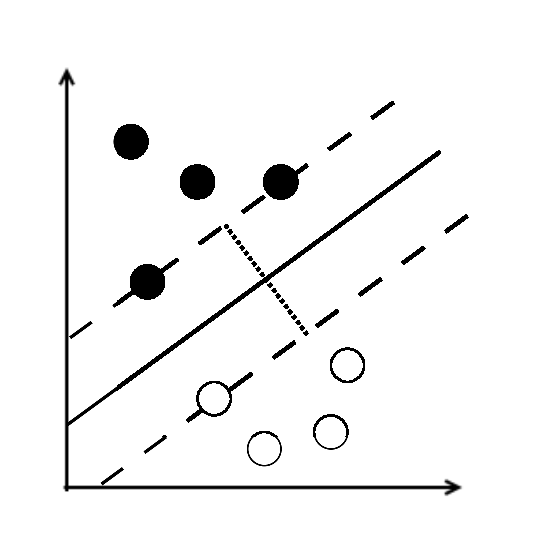
\includegraphics[scale=0.95]{images/method/svm-example.eps}
\caption{An example of a 2-dimensional SVM.}
\label{fig:svm}
\end{figure}

Figure \ref{fig:svm} shows an example of a two-dimensional feature space, with
two classes of points (black and white). We can see the hyperplane, in this
case a line since we are only in two dimensions, separating the two classes
with as much margin as possible. In
this case, the points are linearly separable: all white points lie on one side
of the hyperplane, and all black points lie on the other. In practice, this is
not common, and often data cannot be separated cleanly by a hyperplane.
Note that the points closest to the margin are those that are most likely to be
ambiguous when the data cannot be cleanly separated. The SVM will progressively
remove more and more of these ambiguous points from consideration when it
cannot find a hyperplane until it finds a suitable one.

Instead of removing points from consideration by the SVM, we can also specify
a \textit{kernel function}, which transforms the original feature space into
some other non-linear space. Commonly, polynomial functions of degree 2 or
greater are used, and theoretically they can approximate non-linear boundaries
between classes to any arbitrary accuracy. However, this is usually not
practically possible with data sets containing even a modest number of features
(around 10), due to the computational complexity of estimating a large number
of coefficients that are introduced by the transformation.

SVMs can be specified mathematically as a type of optimisation problem known
as \textit{constrained quadratic optimisation}. Given $m$ training vectors
$\mathbf{x_i} \in \mathbb{R}^n, i=1,\ldots,m$ and their labels
$y_i \in \{-1,+1\}, i=1,\ldots,m$, the optimisation problem can be written as:
\begin{equation*}
\begin{aligned}
& \underset{\mathbf{w},b}{\mathrm{minimise}}
  && ||\mathbf{w}|| + C\sum_{i=1,\ldots,m} s_i \\
& \text{subject to}
  && y_i(\mathbf{w}^T\phi(\mathbf{x_i})+b) \geq 1 \\
& && s_i \geq 0, i = 1,\ldots,m
\end{aligned}
\end{equation*}
where $\phi(\mathbf{x})$ is the kernel function, and
$\mathbf{w}\cdot\mathbf{x_i} + b = 0$ is the hyperplane that the SVM finds.
The $s_i$'s allow the SVM to ignore some examples if it cannot find a suitable
hyperplane, and $C$ (sometimes called the SVM's complexity constant) is a
constant specified by the user that controls how much we want to balance
finding the best possible margin with allowing misclassified examples.
Note that for a linear kernel, $\phi(\mathbf{x}) = \mathbf{x}$. Training the
SVM involves solving this optimisation problem and obtaining values for
$\mathbf{w}$ and $b$.

To classify an instance $\mathbf{x_{new}}$, we simply find the sign of
$\mathbf{w}\cdot\mathbf{x_{new}}+b$. This will tell us which one of the
two classes the new example belongs to.

\section{$k$-Nearest Neighbour}
In this section we will describe the $k$-nearest neighbour ($k$-NN) algorithm
and discuss some extensions which we use in our work. Additionally, we will
describe our contribution, which is an extension of the distance metric for
finding the nearest neighbours.

\subsection{Basic Algorithm}
The $k$-nearest neighbour classifier is an example of an
\textit{instance-based} learning algorithm. This is because it does not, unlike
the other classifiers described in this section, attempt to deduce or
generalise a relationship between the features and the class: it simply stores
all training examples and classifies an unseen example by finding the $k$
``nearest'' examples (or \textit{instances}) and assigning the majority class
to the new example. In the simplest form of the algorithm, $k$ is chosen to be
1 and the Euclidean distance is used to measure the closeness of neighbours:
\begin{equation*}
\mathrm{Distance} = \sqrt{(x_1-y_1)^2 + (x_2-y_2)^2 + \ldots + (x_n-y_n)^2}
\end{equation*}
where $x_i,y_i$ are the values of the $i$-th feature for two different feature
vectors (or instances).

Like the Na\"{i}ve Bayes classifier, $k$-NN allows all features to be taken
into account equally when classifying a new example. However, since feature
values often span different ranges and units of measurement, a particularly
large range of values for a feature would contribute much more to the distance
than another feature that spans a lower set of values.
To avoid this, it is important to \textit{normalise} the
values of each numeric feature before using $k$-NN: for each feature $i$, we
calculate the normalised value of the feature for each training example. This
is done using the following relationship:
\begin{equation*}
a_i = s\left(\dfrac{v_i - \mathrm{min }v_i}{\mathrm{max }v_i - \mathrm{min }v_i}\right) + t
\end{equation*}
where $a_i$ is the normalised value, $v_i$ is the actual value in the data
set, max $v_i$ and min $v_i$ are taken over all training examples, $s$ is a
scaling factor $t$ indicates how much to translate the range by. If $s=1$
and $t=0$, then the range of normalised values will be in $[0,1]$.

\subsection{Existing and Proposed Extensions}
There have been many extensions proposed to the $k$-NN algorithm described
above. These usually seek to find a more suitable distance metric for the
problem domain at hand, or to reduce the storage requirements of the original
$k$-NN algorithm. We will focus on two extensions to the Euclidean distance:
K* and our proposed distance function, Ranked Distance.

\subsubsection{K*: Instance-based Classifier with Entropic Distance Function}
Cleary and Trigg developed K*, an instance-based classifier that uses entropy
to measure the distances between instances \cite{Cleary1995}. They consider
the distance between two instances to be the complexity of transforming one
into another. Define a sequence of transformations on an instance:
\begin{equation*}
\bar{t}(a) = t_n(t_{n-1}(\ldots t_1(a)\ldots)), \bar{t} \in T
\end{equation*}
where $\bar{t} = t_1,\ldots,t_n$. We can define a probability function $p$
that gives the probabilities of these transformations occurring, and then we
can define a probability function that gives the probabilities of all paths
(transformations) from example $a$ to $b$:
\begin{equation*}
P^*(b|a) = \sum_{\bar{t}\in T:\bar{t}(a)=b} p(\bar{t})
\end{equation*}
Within this framework, we can define transformations for both real-valued and
categorical features, which allows K* to work with all types of features.
The K* function is then defined as:
\begin{equation*}
K^*(b|a) = -\mathrm{log}_2P^*(b|a)
\end{equation*}

To calculate the probability of an instance $a$ being in a class $C$, we sum
the probabilities from $a$ to each instance of $C$, and repeat for each class.
The predicted class will be the one with the highest probability:
\begin{equation*}
P^*(C|a) = \sum_{b\in C} P^*(b|a)
\end{equation*}

We use K* as a comparison to the basic NN algorithm and also as a comparison
to $k$-NN with our distance function.

\subsubsection{Proposed Approach: Ranked Distance}
\label{sec:rankeddist}
\paragraph{Intuition}
As we mentioned earlier, all features are considered equally in a $k$-NN
classifier, which implies that all features are equally important in predicting
the class. In practice, however, this is not always the case: to predict the
LOS of a trauma patient, the severity of their injury should affect the final
LOS more than whether or not they can speak English (which could be just two
of many features that are recorded about a patient). Our contribution is thus
a modified distance function to take the relative importance of attributes into
account. 

\paragraph{Mathematical formulation}
Given two instances $\mathbf{x} = (x_1,x_2,\ldots,x_n)$ and
$\mathbf{y} = (y_1,y_2,\ldots,y_n)$, the distance between them is given by:
\begin{equation*}
\mathrm{Distance} = \sum_{i=1}^n w_i |x_i-y_i|
\end{equation*}
where the $w_i$s weight the contribution of the $i$-th feature to the overall
distance that is computed by the $k$-NN algorithm. We assume that all feature
values have been normalised, as described above.

\paragraph{Assignment of weights}
The weights $w_i$ can be tuned to match the particular problem that is being
investigated. For our LOS classification problem, we will consider two ways
of weighting features:
\begin{enumerate}
\item The weight of each feature is the magnitude of the correlation
coefficient
between it and the class, meaning that features that are more highly correlated
with the class will contribute more to the distance. The correlation
coefficient $r_i$ for feature $i$ with the class $c$ can be computed by:
\begin{equation*}
r_i = \dfrac{\sum_{i=1}^m (x_i-\bar{x})(c-\bar{c})}{\sqrt{(\sum_{i=1}^m x_i-\bar{x})(\sum_{i=1}^m c-\bar{c})}}
\end{equation*}
where $m$ is the number of training examples, $x_i$ is the value of feature
$i$, and $\bar{x}$ and $\bar{c}$ are the arithmetic averages of the feature
values and the class values respectively. 
\item We compute the correlation coefficients as described in the point above.
This gives us a ranking of the importance of each feature to the prediction of
the class, with 1 being the highest rank (indicating the most importance) and
$n$ being the lowest rank (indicating the least importance).
Instead of using the values of the correlation directly to weight
the distance contribution of each feature, we specify a function:
\begin{equation*}
f : \mathrm{Rank} \rightarrow \mathbb{R}, \mathrm{Rank} \in \{1,2,\ldots,n\}
\end{equation*}
that describes
how the weights of the features vary with the rank. This function should
inituitively be non-increasing and should produce lower values when the rank
number is greater, meaning that less important features have a lower weight
in the distance calculation.
Note that choosing $f(\mathrm{Rank}) = k$ for any non-zero constant $k$
results in all features contributing equally to the distance calculation.

\noindent We will use $f(\mathrm{Rank}) = \frac{1}{\mathrm{Rank}^c}$, where
$c$ varies from 0 to 1.
\end{enumerate}

\section{Multi-layer Perceptron}
Multi-layer perceptrons (MLPs) are a generalised form of the
\textit{perceptron}, first
studied extensively by Rosenblatt \cite{Rosenblatt1962}. The original
motivation of the perceptron 
was to develop a very simple artificial neural network to model the
behaviour of neurons in the brain. The perceptron model for a two-class
problem is a linear combination of the features: that is,
$h(\mathbf{x}) = \sum w_i x_i$ where the $w_i$ are the weights of the model.
There is an input node, called a \textit{neuron}, for each feature, and the
weights are applied to the connections between these input neurons to the
output.
Usually, a constant term of 1 called the \textit{bias} is also added to the
model for an additional trainable input. To classify an item, we substitute it
into $h(\mathbf{x})$; if the value is above a particular threshold, we label it
as class 1, else it belongs in class 2. For convenience, we can let this
threshold be 0. Training the perceptron involves the following steps:
\begin{enumerate}
\item Start with random numbers for the weights $w_i$.
\item For each training example $\mathbf{x_i}$: calculate $h(\mathbf{x_i})$.
If it is correctly classified, do not update the weights.
If it is incorrectly classified, add a multiple of the misclassified
instance to the current weights using
$\mathbf{w} = \mathbf{w} + \lambda \mathbf{x_i}$, where $\lambda$ is a small
constant.
\item Repeat the previous step until all training examples are correctly
classified.
\end{enumerate}
If the data are linearly separable, the perceptron is guaranteed to find a
hyperplane that separates the two classes. However, it is not able to do this
when there is a non-linear decision boundary -- for that we will need the
multi-layer perceptron.

The \textit{multi-layer perceptron}, also known as a
\textit{feed-forward neural network}, is a type of artificial neural network
that generalises the perceptron model outlined above. Instead of only one layer
of inputs, MLPs consist of more than one layer, with the outputs from previous
layers serving as inputs to the next layer. At each layer, the inputs are
combined linearly and then transformed nonlinearly for input into the next
layer. For a network with one layer of transformations between the input and
output layers -- that is, one ``hidden'' layer -- the mathematical description
is:
\begin{equation*}
y = \sum_j w^{(2)}_j f_j \left(\sum_i w^{(1)}_i x_i\right)
\end{equation*}
The $w$ and the $f_j$ represent the linear combinations and the nonlinear
transformations respectively, and $y$ is the predicted outcome.
The nonlinearity of the transformations ensures
that we can classify data which are not linearly separable. Figure
\ref{fig:mlp} shows an MLP with one hidden layer.

\begin{figure}[h]
\caption{An MLP with one hidden layer.}
\label{fig:mlp}
\centering
%\includegraphics[scale=0.95]{images/a2-nn}
\end{figure}

MLPs can be trained in a number of ways, the most common of which is
\textit{backpropagation}. Suppose that we have the network above, with one
input, hidden and output layer respectively. From the perceptron learning
algorithm, we can update the weights of the hidden neurons leading to the
output neuron, but we do not know what the outputs of these hidden neurons are.
Backpropagation solves this problem by updating the weights of the various
connections to the hidden units based on the strength of the unit's
contribution to the final prediction, using a mathematical optimisation
algorithm called \textit{gradient descent}. This requires taking derivatives,
so the threshold function we used for the perceptron is usually replaced with
the sigmoid function $f(x) = \frac{1}{1+e^{-x}}$. We also define an error
function $E=\frac{1}{2}(\text{actual} - \text{predicted})^2$ -- the one most
commonly used -- which is
minimised in the gradient descent process. Updating the weights for each
connection in the network now involves finding the value of the derivative,
multiplying it by a small constant between 0 and 1 called the
\textit{learning rate}, and subtracting this value from the current weight
value, until the minimum for the error function is reached. Note that the
error function is quadratic, so it is guaranteed to have a minimum. The
updating of the weights is continued until the minimum is reached or if we
are ``close enough'' to the minimum.

It can be shown that MLPs with a single hidden layer are powerful enough to
model any continuous function, provided there are enough neurons in that
hidden layer \cite{Hand2001}. However, as they must iterate over the entire
data set many times, and due to the sometimes slow convergence of gradient
descent, MLPs are often slower to train than other learning algorithms we
have described, such as decision trees. We use them in this work on LOS
classification as we would like to see how they perform in modelling the
complex relationships between various medical attributes.

\section{Summary}
In this chapter we have outlined all of the learning algorithms that we will
be evaluating with respect to our classification problem, from the simple
Zero-R and 1R to Na\"{i}ve Bayes, decision trees, logistic regression,
$k$-nearest neighbour (and extensions K* and Ranked Distance), to the more
sophisticated support vector machines and multi-layer perceptrons. The reason
for our inclusion of so many algorithms is two-fold. Firstly, many of
these algorithms have not been extensively applied in various medical settings
to the problem of LOS prediction. Using a wide range of algorithms from various
paradigms will enable us to see what algorithms perform better than others.
Secondly, evaluating several classifiers will allow us to make comparisons
between different feature selection methods that are independent of the
classifier and give us more insight into the nature of the data set and of the
problem.

\chapter{Feature Preprocessing} \label{chap:preprocess}

In the previous chapter we began by describing each training example as a
vector of feature values, and then described how a range of different
learning algorithms used those feature vectors to learn a way to
distinguish examples of one class from another. However, it is uncommon that
data can be used in a learning algorithm without first being preprocessed.
Preprocessing involves cleaning and transforming the data, and is critical
to the performance of learning algorithms that are applied to it. Without
preprocessing, it will be difficult to evaluate the true performance of
our classifiers on the data set and to draw meaningful conclusions from
comparisons between classifiers.

In this chapter we introduce the data sets and give an overview of
preprocessing, describing the specific steps we took on our data.

\section{Data Sets}
In our work we obtained two independent sets of LOS data, one specifically for
trauma and the other a general, hospital-wide set.

\subsection{Trauma LOS Data}
\subsubsection{Collection}
The data set used consisted of trauma registry data from the trauma centre
at the Royal Prince Alfred Hospital, a major trauma centre in New South Wales,
Australia. It covered all adult (age 15 and over) inpatient admissions to the
trauma centre from 2007--2011. 

All patients were first admitted to the trauma ward until discharged
or transferred to an appropriate unit within the hospital. A single trained
data manager recorded a variety of attributes about the admitted patient,
such as age, gender, blood pressure, mechanism of injury and body regions
that were injured. We received this data in a Microsoft Excel spreadsheet.

\subsubsection{Characteristics}
There were 2546 patient records in the data set we received, comprising of 79
features, one of which was the target variable \texttt{los48}.
\texttt{los48} was a binary variable -- that is, it could only take two
values, 0 or 1 -- with 1 indicating that the patient stayed two days or less,
and 0 indicating a stay of greater than 2 days.

\subsubsection{Features}

\subsection{General Hospital LOS Data}
By collaborating with our colleagues from the University of Minho in Portugal,
we were able to obtain LOS data for all inpatient hospitalisations from
2000--2013 at the Hospital das Foras Armadas in Lisboa, Portugal. The data
contained 26462 inpatient records spanning all medical departments within the
hospital, comprising 15 features that were not specific to any medical domain.

\subsubsection{Features}

\section{Cleaning} % missing values, irrelevant features
In any data mining task, adequately \textit{cleaning} the data ensures the best
chance of success: this includes deciding how to deal with missing and
inaccurate values, as well as appropriately transforming the data
\citep{Witten2005}.
The exact steps involved in data cleaning will vary between data
sets, but the overall process is similar. Common issues to deal with include:
\begin{itemize}
\item Incorrect spelling or punctuation, perhaps as a result of mistakes in
data entry
\item Leading or trailing whitespace, and other garbage characters,
perhaps as a result of data entry or
the system that stores the data
\item Missing values for various features or for the class label
\item Values for features that do not make sense (such as a patient age of
-1)
\end{itemize}
The following paragraphs address how we dealt with the issues that were
applicable to our data.

\paragraph{Incorrect spelling and punctuation.}
Since the data was initially in Excel spreadsheet format, we explored the data
by hand using Microsoft Excel's filter on each column. This allowed us to see
the range of possible values for each feature and easily detect anomalous
selling and punctuation:
\begin{itemize}
  \item In the \texttt{sex} attribute, there were values of `Female' and
  `Femal' which were consolidated into `Female'.
  \item In the \texttt{mechanism} attribute, which was textual and indicated
  the category of how the patient was injured, there were such categories as
  `Other Vehi' and `Other Vehicle' as well as `Pedal Cycl' and `Pedal Cyclist'.
  Such categories were combined into `Other Vehicle' and `Pedal Cyclist'
  respectively.
  \item Some categories in \texttt{mechanism} were also divided into whether or
  not the mechanism of injury was self-inflicted, such as `Shooting' and
  `Shooting-selfinflicted'. At the suggestion of a domain expert, we combined
  them into one category: in this case, simply
  `Shooting'; this was done for all the categories in this attribute.
  \item \texttt{disp from ED} indicated the section of the hospital that the
  patient was discharged to. This was also a textual categorical attribute.
  There were redundancies like `G. ICU' and `G.ICU' and even `GICU', which we
  all combined into one category, `GICU'.
\end{itemize}

\paragraph{Extraneous whitespace or other characters.}
After correcting for spelling and punctuation errors,
the data was then exported into CSV (comma-separated value) format, so that
we could continue to process it programmatically rather than manually without
having to use Excel. Many
fields in the data set contained leading or trailing whitespace, which was
removed with a few lines of Python code (see appendix \todo{[add reference
to appendix]}). All attribute names were converted to lowercase. In the case
where attribute names consisted of several words, the spaces were replaced
with underscores (\_) to ensure that the full attribute name was read.
For example, \texttt{Any Cancer} was converted into \texttt{any\_cancer}.

\paragraph{Missing values.}
There has been a varied treatment of missing values in the work of other
researchers, from discarding examples with missing values for any feature
to \textit{imputing} or ``filling in'' the missing values. We remove all
examples with missing feature values from consideration in all further
investigations, in line with the work of other research in LOS prediction
in the same domain \cite{Dinh2013a}.

At the end of the cleaning process, the data was converted into the
Attribute-Relation File Format (ARFF)
\footnote{\url{http://www.cs.waikato.ac.nz/ml/weka/arff.html}} for use in
WEKA, a suite of machine learning algorithms implemented in Java
\cite{Hall2009}. Each feature was carefully checked to ensure that their
type was specified correctly -- that is, the nominal attributes were
distinguished from the numeric.

\section{Normalisation}
Features represent different pieces of information about a training example.
Therefore, it is not surprising that not all features will have the same range
of values: a patient can have an \texttt{age} feature with a value of 20, but
their \texttt{heart rate} feature cannot possibly be 20. Learning algorithms
such as $k$-nearest neighbour (Chapter \ref{chap:classification})
are sensitive to the scales of feature values -- features with a larger range
of values will dominate a distance calculation. Therefore, we
\textit{normalise} all numeric (that is, continuous-valued)
feature values into the $[-1,1]$ range so that they are all expressed on the
same scale. Typically, values are normalised in the $[0,1]$ or the $[-1,1]$
ranges.
The formula to do this, also discussed in Chapter \ref{chap:classification},
is:
\begin{equation*}
a_i = 2\left[\dfrac{v_i - \mathrm{min }v_i}{\mathrm{max }v_i - \mathrm{min }v_i}\right] - 1
\end{equation*}
where we have used $s=2$ and $t=-1$ to transform values into the $[-1,1]$
range. This transformation was applied to each value of all numeric features
using WEKA, and was performed after all cleaning steps described above.

\section{Discretisation}
Not all classification algorithms can handle numeric features, and some of the
ones that do require assumptions to be made about the underlying distribution
of the feature values that is not always satisfied -- recall the normality
assumption of the Na\"{i}ve Bayes classifier
from Chapter \ref{chap:classification}. This requires us
to \textit{discretise} the numeric features, which is a process of splitting
the continuous data into a small number of discrete, distinct ranges.
Additionally, there has been no work examining the use of discretisation to
improve the performance of LOS prediction models, so our work provides a
valuable guideline on what other researchers looking at a similar problem can
expect.

Two basic approaches to the discretisation problem exist: unsupervised and
supervised. \textit{Unsupervised} discretisation involves splitting each
feature without considering any class information, whereas \textit{supervised}
discretisation accounts for the class when discretising.
Unsupervised discretisation uses simple methods such as splitting the data into
fixed-width intervals -- each interval spans the same width of values,
but can contain different numbers of feature values depending on the
distribution of underlying data -- which
can often partition the continuous feature into unhelpful categories due to its
ignorance of class labels. Supervised discretisation, on the
other hand, is commonly performed using the entropy minimisation heuristic
described by Fayyad and Irani \cite{Fayyad1993}. Since we have labelled
data, we are able to use both approaches. However, we will focus on evaluating
the effect of supervised discretisation, as it is generally preferred to
unsupervised discretisation when class information about the training examples
is known. And the method proposed by Fayyad and Irani is one of the best known
general supervised discretisation techniques \cite{Witten2005}.

\subsection{Entropy-based Discretisation}
In Chapter \ref{chap:classification} we outlined the induction of a decision
tree on a data set, using the information gain as the criterion for deciding
the attribute to split on at each step. A similar approach is used in Fayyad
and Irani's entropy-based method of discretisation \cite{Fayyad1993}:
to discretise an attribute,
each possible split point is considered and the information gain from that
split is computed. The split point with the highest information gain is
therefore chosen. Once the first split is determined, the algorithm continues
recursively in the newly created upper and lower ranges.

The \textit{minimum description length (MDL)} principle is used to determine
the stopping criterion. The MDL value is calculated by adding the information
values from two cases: split or do not split. If we split, then we can encode
the split point in $\mathrm{log}_2(N-1)$ bits (where $N$ is the number of
instances), then the classes of those above and below it. If we do not split,
then each instance's label must be encoded. Mathematically, given $N$ examples
with entropy $E$, sub-intervals $k_1$ and $k_2$ with the entropy of examples
in each sub-interval denoted $E_1$ and $E_2$:
\begin{equation*}
\mathrm{MDL} = \dfrac{\mathrm{log}_2(N-1)}{N} + \dfrac{\mathrm{log}_2(3^k-2) - kE + k_1E_1 + k_2E_2}{N}
\end{equation*}
The first term is the information needed for the splitting point, and the
second is a correction necessary for encoding which classes belong to which
sub-interval. The decision rule is then to split if the information gain for
that split exceeds the MDL value: $\mathrm{gain} > \mathrm{MDL}$.

Since this requires exhaustive searching of the full range of feature values
to find potential split points, this method of supervised discretisation can
be time-consuming given large enough data sets. However, it has been proven
that any potential split that minimises the information value will never occur
between two examples of the same class. This means that we only need to
consider splits between regions of different classes, reducing the number of
possible points to consider.

The data was discretised according to the above method using the supervised
discretisation filter in WEKA. We keep both the original data set (without
discretisation) and the discretised data set for comparison.

\section{Summary}
In this chapter we discussed various issues encountered during the
preprocessing stage and how these were addressed. These steps are critical to
the success of our learning algorithms: without cleaned data, any subsequent
work is meaningless and difficult to draw valid conclusions from. By outlining
our steps, we hope to provide an example of how one can conduct the cleaning
process.

We then discussed normalisation, an important transformation of
continuous-valued data that ensures all features take on the same range of
values. This is important for ensuring that classifiers sensitive to the
relative range of values between features give valid outputs.

We concluded with outlining discretisation, in particular Fayyad and Irani's
entropy-based method. Such a technique has not been used in LOS prediction
and by including it in our work, we can evaluate its effectiveness in this
domain and let our results serve as a baseline and reference for future work.

\chapter{Feature Selection} \label{chap:selection}

Recall that each feature tells
us something about a training example. Ideally, it should also help us
classify the example. However, in practice and particularly
in medicine, a large number of attributes about a patient is usually recorded,
not all of which are relevant in predicting the class.
Having such a large number of features
is detrimental for two reasons: the training time is significantly
increased because the classifier must incorporate more information than it
needs to, and
this irrelevant information tends to degrade the performance
of even state-of-the-art classifiers such as C4.5 decision trees
\cite{Witten2005}. Clearly, there is an advantage in considering only a subset
of the most relevant features; to find them, we will use what is called
\textit{feature selection}.

Our data set contains 78 features aside from the class, which is a fairly high
number. Many of these attributes
are derived from others in the set: for example, whether or not a patient is
over 65 years of age (the \texttt{age65} feature) is directly dependent on the
value of their \texttt{age} attribute.

\section{Preliminary Removal of Features}
We began the process of feature selection by removing attributes that were
not available upon admission, as these tended to be highly related to the
\texttt{los48} outcome and were a consequence, not a predictor, of LOS. Had
we not removed these features, they would be selected by the feature selection
methods described below due to their high association with \texttt{los48}, but
would actually tell us nothing about what causes a patient to require a
hospital stay of more or less than 2 days.
These attributes were: \texttt{iculos}, \texttt{outcome},
\texttt{disp from ed}, \texttt{disp from hosp}, \texttt{died}, \texttt{rehab},
\texttt{los} and \texttt{eddc}.
The \texttt{id} attribute was also removed because it
simply numbered each record and
indicated nothing about the patient. This left us with 69 attributes.

We then removed 10 other features which were directly derived from others in
the data set: \texttt{gcs1}, \texttt{iss8}, \texttt{mechanism}, \texttt{male},
\texttt{age65}, \texttt{bp1}, \texttt{pr1}, \texttt{rr1}, \texttt{fall} and
\texttt{comorbidity}. At this stage there were 59 features -- still a large
number.

After eliminating redundant or inapplicable features as detailed above, we
considered four \textit{automatic} (correlation-based
feature selection, Pearson correlation, 1R and wrapper selection
using C4.5) and two \textit{manual} feature selection methods (domain expert
selection and the feature set used in existing work on trauma LOS prediction).
These methods are described in the following sections.

\section{Automatic Methods}
Automatic feature selection methods are useful for when we do not have a deep
understanding of the underlying domain and what each attribute really means to
the class. Even if we are well-versed in the domain, evaluating a few different
methods of automatic feature selection can give us new insight into the
learning problem at hand. Here we will describe a few of the methods we used.

\subsection{Correlation-based Feature Selection (CFS)}
Correlation-based feature selection (CFS) is a method developed by Hall
\cite{Hall2000} which looks for a subset of features that have high correlation
with the class but low intercorrelation among the features. In this case,
correlation between two features is measured using what is called the
\textit{symmetric uncertainty}:
\begin{equation*}
U(A,B) = 2\dfrac{H(A)+H(B)-H(A,B)}{H(A)+H(B)}
\end{equation*}
where $A$ and $B$ are two nominal attributes and $H$ is the entropy function
denoted by Equation \ref{eqn:entropy} in Chapter \ref{chap:classification}.
The entropies are calculated from the probabilities of each feature value, and
$H(A,B)$, the joint entropy of $A$ and $B$, is calculated from the
probabilities of each combination of values of $A$ and $B$. Note that $U(A,B)$
is always between 0 and 1.

To evaluate the ``goodness'' of a subset of features with the class $C$, we
compute:
\begin{equation}
\label{eqn:cfs}
\dfrac{\sum_j U(A_j,C)}{\sqrt{\sum_i \sum_j U(A_i,A_j)}}
\end{equation}
where $i$ and $j$ range over the features in the subset being evaluated. The
maximum value that Equation \ref{eqn:cfs} can obtain is 1 when all features
correlate perfectly with the class and also with each other -- the numerator
becomes $n$ and the denominator $\sqrt{n^2}$ if the subset has $n$ features.
\todo{elaborate a bit more}

\subsection{Pearson Correlation Coefficient}
The Pearson correlation coefficient measures the degree of linear correlation
between two variables. It is always in the range $[-1,1]$, where -1 is total
negative correlation, 0 is no (linear) correlation, and 1 is total positive
correlation. We compute the Pearson correlation between each feature and the
class using:
\begin{equation*}
r_i = \dfrac{\sum_{i=1}^m (x_i-\bar{x})(c-\bar{c})}{\sqrt{(\sum_{i=1}^m x_i-\bar{x})(\sum_{i=1}^m c-\bar{c})}}
\end{equation*}
where $m$ is the number of training examples, $x_i$ is the value of feature
$i$, and $\bar{x}$ and $\bar{c}$ are the arithmetic averages of the feature
values and the class values respectively. (Recall that we also used this
in Chapter \ref{chap:classification} to rank features for use in Ranked
Distance nearest neighbours.) 

A higher value for $r_i$ indicates higher correlation with the class. We
rank all features according to their $r_i$ from highest to lowest, and select
some subset of these either by selecting a fixed number, or selecting all
features that have a correlation above a specified threshold.

\subsection{1R}
Another way to evaluate the relevance of features is to use the idea behind the
1R classifier described in Section \ref{sec:zeror}. Recall that the 1R
classifier constructs simple 1-rules based on each feature and uses the feature
that produces the lowest error rate (that is, the highest accuracy) on the data
set to classify unseen examples. These accuracy rates can be calculated for
each feature, which are then used to rank the features from highest to lowest
accuracy. The worst accuracy for any feature is the 0R accuracy, which is the
proportion of the majority class in the data set. This is because if 1R finds
that the accuracy of the rule constructed using a feature is worse than 0R,
then it will not use that rule and predict the majority class instead.

We can also select a fixed number of features or all features above a certain
1R accuracy threshold.

\subsection{Wrapper-based Feature Selection}
The feature selection methods described above (CFS, Pearson correlataion and
1R) have been described as \textit{filter} approaches to attribute selection.
Kohavi and John proposed another approach, the \textit{wrapper} approach:
instead of performing feature selection independently of the learning
algorithm using some measure of ``relevance'',
the learning algorithm itself is used to evaluate the goodness of
subsets of features \cite{Kohavi1997}. The difference between the filter
and wrapper approaches is depicted in Figure \ref{fig:wrapper}.

\begin{figure}[h]
\label{fig:wrapper}
\caption{}
\centering
%\includegraphics[scale=0.95]{images/a2-nn}
\end{figure}

A key advantage of the wrapper approach is that the selected feature sets are
specifically tailored to a learning algorithm, which ensures the best
performance of that algorithm given the data set. However, wrapper approaches
can also be prohibitively slow if the data or feature sets are large and the
chosen learning algorithm expensive to train (such as support vector machines
and multi-layer perceptrons). We will evaluate the use of C4.5 decision trees
(see Section \ref{sec:c45}) in selecting features using the wrapper approach.
Using decision trees to select features is relatively fast as due to the
divide and conquer nature of the learning algorithm, and the tendency of the
trees to select fewer features for learning than other algorithms.

\section{Manual Selection}
\label{sec:manual}
All of the above automatic feature selection methods use some notion of
``relevance'', such as symmetric uncertainty and linear correlation,
in order to determine the best subset of features to select.
Depending on the problem at hand, these definitions of relevance may or may
not work well with the data. In the LOS prediction literature, studies
have enlisted the help of medical domain experts to assist in feature
selection, due to their experience and understanding of the underlying
problem and the effect of the features on the outcome. It will therefore be
worthwhile to compare the performance of classifiers using features selected
automatically and manually.

\subsection{Baseline Feature Set}
The key previous work on trauma LOS prediction was by Dinh et. al.
\cite{Dinh2013a}, who used a specific feature set from the data set that we
use. We would like to use the features they selected as a baseline for
evaluating the other feature selection methods we describe.

\subsection{Domain Expert Selection}
Consultation with a domain expert yielded another feature set that we could
use to compare with the baseline and with the other automatic methods.

\section{Conclusion}
In this chapter we covered feature selection, which is concerned with reducing
the number of attributes that a learning algorithm needs to consider when
trying to learn a relationship between the training examples and their labels.
We described how we removed redundant and meaningless features before the
feature selection step, and discussed the automatic and manual feature
selection methods we use in our work. The value in using several methods of
each type of feature selection is two-fold: it allows us to not only compare
the performance of the methods, but also to compare the performance of the
different classifiers we use independently of the feature selection method.

\chapter{Evaluation} \label{chap:evaluation}

The methods of evaluating the performance of classifiers in LOS prediction
that are discussed in the literature encompass a wide range of medical
domains and learning problems, which presents us with a challenge when we
decide how to evaluate our work. Here we have chosen to rigorously evaluate
our results (such as using stratified cross-validation when others may have
used a single training-test split), while still using performance measures
comparable to the literature and suitable for our particular learning problem.
This chapter discusses the data sets, procedure and performance measures used
in evaluating our work.

\section{Data Sets}
In our work we obtained two independent sets of LOS data, one specifically for
trauma and the other a general, hospital-wide set.

\subsection{Trauma LOS Data}
\subsubsection{Collection}
The data set used consisted of trauma registry data from the trauma centre
at the Royal Prince Alfred Hospital, a major trauma centre in New South Wales,
Australia. It covered all adult (age 15 and over) inpatient admissions to the
trauma centre from 2007--2011. 

All patients were first admitted to the trauma ward until discharged
or transferred to an appropriate unit within the hospital. A single trained
data manager recorded a variety of attributes about the admitted patient,
such as age, gender, blood pressure, mechanism of injury and body regions
that were injured. We received this data in a Microsoft Excel spreadsheet.

\subsubsection{Characteristics}
There were 2546 patient records in the data set we received, comprising of 79
features, one of which was the target variable \texttt{los48}.
\texttt{los48} was a binary variable -- that is, it could only take two
values, 0 or 1 -- with 1 indicating that the patient stayed two days or less,
and 0 indicating a stay of greater than 2 days.

\subsection{General Hospital LOS Data}
By collaborating with our colleagues from the University of Minho in Portugal,
we were able to obtain LOS data for all inpatient hospitalisations from
2000--2013 at the Hospital das Foras Armadas in Lisboa, Portugal. The data
contained 26462 inpatient records spanning all medical departments within the
hospital, comprising 15 features that were not specific to any medical domain.

\section{Evaluation Procedure}
\subsection{Steps Involved}
The steps that we took to evaluate the performance of the various classifiers
and feature selection methods were:
\begin{enumerate}
\item The trauma LOS data was cleaned and preprocessed as described in Chapter
\ref{chap:preprocess}, giving us two data sets: one with and one without
discretisation. The general LOS data from Portugal was already cleaned when we
received it; however, we discretised the continuous \texttt{los} variable to
the same categories as for the trauma data (2 days or less, greater than 2
days), normalised the numeric attribute \texttt{prev\_admissions}, and derived
both a discretised and non-discretised data set. This resulted in 4 sets of
data.
\item For each data set, we evaluated the effect of the 4 automatic feature
selection methods on each of the 8 classifiers described in Chapter
\ref{chap:classification}, giving us 32 configurations for each data set, over
4 sets. Evaluation was performed using \textit{ten-fold stratified
cross-validation} (described below).
\item For the two trauma LOS data sets, we additionally evaluated the two
manual feature selection methods with all 8 classifiers. Recall from Section
\ref{sec:manual} that one of the feature sets is from the key previous work
on trauma LOS prediction that we use as a baseline, and the other feature set
is a set of features included through consultation with a domain expert.
\end{enumerate}

\subsection{Ten-fold Stratified Cross-Validation}
Cross-validation is a method of evaluating the performance of a learning
algorithm. The entire data set is partitioned into $k$ subsets, and the
learning algorithm is trained on $k-1$ of these subsets and tested on one. This
is repeated $k$ times, so that each of the subsets is used exactly once as a
test set. After each iteration of training and testing, called a \textit{fold},
various performance measures about the classifier are recorded. At the end of
the $k$ folds, the $k$ performance measures obtained are averaged to arrive at
a final measure of performance. \textit{Stratified} cross-validation ensures
that the proportion of each class in each of the $k$ subsets is approximately
the same as in the entire data set. This reduces the effect of random uneven
class representation in the partitioned $k$ subsets during the cross-validation
process.

We use $k=10$ folds for our stratified cross-validation, which has been
considered the standard method of measuring the performance of a learning
algorithm on a given data set \cite{Witten2005}.

\subsection{Technical Details}
Here we specify the technical details of our work: namely, the programming
languages and software used in our entire procedure.

\subsubsection{Repository}
All code relating to this work, including the \LaTeX code for this document,
as well as results from our evaluations are available publicly online at
\url{https://github.com/tianyupu/hons-thesis}. However, we were not able to
obtain permission from neither the Royal Prince Alfred Hospital nor the
Hospital das Foras Armadas to make the data publicly available due to the
privacy of patient information. Interested readers should discuss with the
author.

\subsubsection{Software Used}
For initial exploration and cleaning of data, we used Microsoft Excel 2007
as the data was already in spreadsheet format. This was then exported to
CSV. For the conversion to ARFF, and evaluation of the automatic
feature selection methods and classification algorithms, we used the latest
developer version of WEKA, 3.7.11 \cite{Hall2009}. We used WEKA exclusively
through the command-line interface so that we could automate and configure
our experiments easily using scripts which we wrote (see Section
\ref{sec:code}).

\subsubsection{Code Written}
\label{sec:code}
\todo{attach code in appendix?}
Leading and trailing whitespace was removed and feature names transformed using
code written in Python to manipulate the CSV. All runs of WEKA were executed by
a program we wrote in Bash (a Unix shell) script. This program was able to run
WEKA with the following features:
\begin{itemize}
\item The ability to specify filenames corresponding to the input training data
and the specification of classification or feature selection algorithms to run
\item ROC curve data output can be optionally enabled and saved to disk after
each cross-validation pass
\item An experiment can be repeated an arbitrary number of times -- this is
specified by the user upon invoking the script (default is one time)
\item The ability to specify the inclusion of a random number seed -- this is
necessary for repetitions of runs to generate different cross-validation splits
\item Model information and performance measures are saved to disk after each
cross-validation
\end{itemize}

Because of the large numbers of results we obtained, we also wrote scripts in
Bash and Python to process and summarise the performance measures we required.
If we ran a set of classifiers 50 times in an experiment, the script would
retrieve all 50 outputs of a performance measure (such as accuracy, described
in the next section) for each classifier, and compute the mean and confidence
interval (also discussed in the next section) in a single output that we could
then save as CSV.

In order to implement our novel Ranked Distance function (Section
\ref{sec:rankeddist}), we created our own class within the WEKA Java package
hierarchy. This was implemented in Java and needed to implement the correct
interfaces and override the right inherited methods in order for the $k$-NN
classifier in WEKA to be able to use it as a distance function. This also
involved updating certain properties of the \texttt{weka.jar} executable in
order to use the new class, as well as building the entire WEKA source. The
development environment we used was Eclipse \todo{insert version}, and the
source was built using the 1.7 Java runtime. \todo{double check}

\section{Performance Measures}
There are many ways to evaluate the performance of learning algorithms. The
two measures we will use are the \textit{accuracy} and the \textit{area under
the receiver operating characteristic (ROC) curve}, commonly abbreviated AUC
(for \textit{area under the curve}).

\subsection{Accuracy}
The accuracy is a common measure of performance for classification algorithms,
and indicates the proportion of examples that were classified correctly from
a given data set. Mathematically, assuming a two-class scenario, the expression
is:
\begin{equation*}
\mathrm{Accuracy} = \dfrac{TP + TN}{TP + TN + FP + FN}
\end{equation*}
where:
\begin{itemize}
  \item $TP$ is the number of \textit{true positives} -- that is, the number of
  examples belonging to class 1 that were classified as belonging in class 1;
  \item $TN$ is the number of \textit{true negatives}, which is the number of
  examples belonging to class 0 that were classified as belonging to class 0;
  \item $FP$ is the number of \textit{false positives}, which is the number of
  examples that should have been classified 0 but were classified as 1; and
  \item $FN$ is the number of \textit{false negatives}, which is the number of
  examples that should have been classified 1 but were classified as 0.
\end{itemize}

The accuracy can also be expressed more simply and intuitively as
$\dfrac{\text{number of correct classifications}}{\text{total number of examples}}$
but the terms introduced above will be necessary to understand the
AUC measure below.

We use accuracy as a performance measure as it is often used in previous work,
which allows us to compare our work with others. Accuracy is also relatively
straightforward to understand and interpret.

\subsection{Area Under the Curve (AUC)}
The area under the receiver operating characteristic (ROC) curve, often
abbreviated AUC, is a measure of the ability of a binary classifier to
distinguish between members of the two classes. Let the \textit{true
positive rate} be $\dfrac{TP}{TP + FN}$ and the \textit{false positive rate}
be $\dfrac{FP}{FP + TN}$. The ROC curve is a plot of the true positive rate
on the vertical axis against the false positive rate on the horizontal axis.
The area under this curve will lie between 0 and 1, with 1 indicating a
100\% true positive rate and 0\% false positives (that is, everything was
classified correctly). The AUC of randomly picking between the two classes
with equal probability is 0.5, with a ROC curve that is a straight line
dividing the graph diagonally in half. Figure \ref{fig:sampleroc} shows
two ROC curves on the same graph:

\begin{figure}[h]
\label{fig:sampleroc}
\caption{}
\centering
%\includegraphics[scale=0.95]{images/a2-nn}
\end{figure}

The AUC has not been commonly used in the literature to evaluate LOS
classification problems, but we have included it in our work for a number of
reasons. Firstly, it measures an aspect of classifiers that accuracy does not,
and which is more important and useful in the domain: the ability to
discriminate between instances of two classes. Recall from Chapter
\ref{chap:classification} that 0R will always predict the majority class --
this means that it will be evaluated positively on the basis of accuracy
as long as there are sufficiently more examples of one class than the other.
However, the AUC of the classifier will be \textit{less} than 0.5, because it
is less able to distinguish between the two classes than random guessing is,
due to the fact that it only ever predicts unseen examples to be in the
majority class. Secondly, previous work on trauma LOS prediction by Dinh et al.
also used the AUC as the key measure by which they evaluated their model
\cite{Dinh2013a}, and we would like our work to be comparable to theirs.

\subsection{Confidence Intervals}
In order to compare our results with that of Dinh et. al. \citep{Dinh2013a},
we are especially interested in the mean cross-validated AUC of our
classifiers as well as
the upper and lower bounds of the 95\% confidence interval associated with this
mean. The intervals are constructed using this argument:

For each classifier, let the population of all of its ten-fold cross-validated
AUC scores be some random variable $X$, which follows a distribution whose
parameters (such as mean and standard deviation) we do not know.
The Central Limit Theorem states that given a random
sample of $n$ items from $X$, namely $X_1,X_2,\dots,X_n$, the sample mean
$\bar{x}$
is approximately normally distributed when $n$ is at least roughly around 30
and the $X_i$'s are independent and identically distributed.
Consequently, we can construct a $(1-\alpha)$\% confidence interval for
$\bar{x}$ -- where $\alpha$ is commonly called the
\textit{significance level} -- as follows:
\begin{equation*}
  \left[\bar{x} - z_{1-\alpha/2}\dfrac{s}{\sqrt{n}},
    \bar{x} + z_{1-\alpha/2}\dfrac{s}{\sqrt{n}}\right]
\end{equation*}
where $\bar{x}$ is the sample mean, $\alpha$ is the significance level
(5\% or $0.05$ in our case), $s$ is the sample standard deviation, $n$
is the number of observations in our sample, and $z_{1-\alpha/2}$ is the value
of the standard normal variable $Z \sim \mathcal{N}(0,1)$ with cumulative
probability $1-\alpha/2$. Since we have taken 40 independent samples of the
ten-fold cross-validated AUC, the Central Limit Theorem holds and we can
compute the mean and standard deviation of our 40 samples in order to
construct a 95\% confidence interval for the mean AUC of each classifier.

\subsection{Tests for Statistical Significance}
To decide whether or not the difference in values of each measure between
classifiers and feature selection methods was statistically significant,
paired $t$-tests at a significance level of 0.05 were conducted.
\todo{elaborate}

\section{Summary}
In this section we described our method of evaluating the performance of each
classifier and feature selection method that we use. We used accuracy and the
area under the curve to measure two different aspects of our classifiers, and
we obtained these figures using stratified ten-fold cross-validation. Paired
$t$-tests were conducted to test for statistical significance.

\chapter{Results and Discussion} \label{chap:results}

\section{Overall Performance}
\subsection{Trauma Data Set}
Tables \ref{tab:overall-tr-acc} and \ref{tab:overall-tr-auc} show the best
accuracy and AUC results for each of the feature selection methods for each
classifier. The best accuracy was 77.81\%, achieved using the $k$-NN algorithm
with 1 nearest neighbour, a discretised data set, and feature selection using a
C4.5 wrapper. The best AUC of 0.846 was achieved using logistic regression with
features selected by a correlation coefficient threshold of 0.1, and again
using the discretised data set.

\begin{table}[htbp]
\caption{Overall best accuracy of each classifier with a particular feature selection method on the trauma data set. * indicates that results were identical regardless of discretisation. D indicates that discretisation was used, and $t$ is the threshold at which the feature selector was applied. The absence of * or D means that not discretising produced a better result. The best result for each classifier is highlighted in bold, with ties broken in favour of the smallest feature set.}
\label{tab:overall-tr-acc}
\resizebox{\linewidth}{!}{%
\begin{tabular}{|l|cccccccc|}
\hline
Classifier & None & Baseline & Expert & CFS & C4.5 Wrapper & Correlation & IG & 1R \\ \hline
ZeroR & 66.91* & 66.91* & 66.91* & 66.91* & 66.91* & 66.91* & 66.91* & 66.91* \\
1R & 71.95 & 66.91* & \begin{tabular}[c]{@{}c@{}}70.64\\ D\end{tabular} & \textbf{72.01} & 71.93 & \begin{tabular}[c]{@{}c@{}}71.91\\ t=0.01\end{tabular} & \begin{tabular}[c]{@{}c@{}}71.95\\ t=0.001\end{tabular} & \begin{tabular}[c]{@{}c@{}}71.97\\ t=66.905\end{tabular} \\
NB & \begin{tabular}[c]{@{}c@{}}73.83\\ D\end{tabular} & 74.62* & \begin{tabular}[c]{@{}c@{}}73.19\\ D\end{tabular} & \begin{tabular}[c]{@{}c@{}}73.4\\ D\end{tabular} & \textbf{\begin{tabular}[c]{@{}c@{}}75.8\\ D\end{tabular}} & \begin{tabular}[c]{@{}c@{}}74.85\\ D, t=0.125\end{tabular} & \begin{tabular}[c]{@{}c@{}}74.45\\ D, t=0.01\end{tabular} & \begin{tabular}[c]{@{}c@{}}72.37\\ D, t=69.905\end{tabular} \\
DT & \begin{tabular}[c]{@{}c@{}}75\\ D\end{tabular} & 74.38* & \begin{tabular}[c]{@{}c@{}}76.39\\ D\end{tabular} & 75.4 & \textbf{\begin{tabular}[c]{@{}c@{}}77.52\\ D\end{tabular}} & \begin{tabular}[c]{@{}c@{}}76.05\\ D, t=0.11\end{tabular} & \begin{tabular}[c]{@{}c@{}}76.17\\ D, t=0.01\end{tabular} & \begin{tabular}[c]{@{}c@{}}73.49\\ t=66.905\end{tabular} \\
LR & \begin{tabular}[c]{@{}c@{}}77.62\\ D\end{tabular} & 75.06* & \begin{tabular}[c]{@{}c@{}}76.45\\ D\end{tabular} & 74.14 & \begin{tabular}[c]{@{}c@{}}76.3\\ D\end{tabular} & \textbf{\begin{tabular}[c]{@{}c@{}}77.7\\ D, t=0\end{tabular}} & \begin{tabular}[c]{@{}c@{}}77.65\\ D, t=0\end{tabular} & \begin{tabular}[c]{@{}c@{}}74.4\\ D, t=66.905\end{tabular} \\
SVM & \begin{tabular}[c]{@{}c@{}}77.39\\ D\end{tabular} & 74.47* & \begin{tabular}[c]{@{}c@{}}75.67\\ D\end{tabular} & \begin{tabular}[c]{@{}c@{}}72.57\\ D\end{tabular} & \begin{tabular}[c]{@{}c@{}}75.26\\ D\end{tabular} & \begin{tabular}[c]{@{}c@{}}77.42\\ D, t=0.1\end{tabular} & \textbf{\begin{tabular}[c]{@{}c@{}}77.53\\ D, t=0.005\end{tabular}} & \begin{tabular}[c]{@{}c@{}}73.83\\ D, t=66.905\end{tabular} \\
1NN & \begin{tabular}[c]{@{}c@{}}71.22\\ D\end{tabular} & 70.28* & \begin{tabular}[c]{@{}c@{}}72.56\\ D\end{tabular} & 74.44 & \textbf{\begin{tabular}[c]{@{}c@{}}77.81\\ D\end{tabular}} & \begin{tabular}[c]{@{}c@{}}74.75\\ D, t=0.15\end{tabular} & \begin{tabular}[c]{@{}c@{}}73.26\\ D, t=0.01\end{tabular} & \begin{tabular}[c]{@{}c@{}}73.78\\ t=68.905\end{tabular} \\
20NN & \begin{tabular}[c]{@{}c@{}}75.9\\ D\end{tabular} & 73.59* & \begin{tabular}[c]{@{}c@{}}75.51\\ D\end{tabular} & 75.3 & \begin{tabular}[c]{@{}c@{}}76.48\\ D\end{tabular} & \begin{tabular}[c]{@{}c@{}}76.26\\ D, t=0.125\end{tabular} & \textbf{\begin{tabular}[c]{@{}c@{}}76.56\\ D, t=0.005\end{tabular}} & \begin{tabular}[c]{@{}c@{}}73.56\\ t=68.905\end{tabular} \\
RD & \begin{tabular}[c]{@{}c@{}}76.92\\ D\end{tabular} & 69.68* & \begin{tabular}[c]{@{}c@{}}76.19\\ D\end{tabular} & 74.38 & \textbf{\begin{tabular}[c]{@{}c@{}}77.22\\ D\end{tabular}} & \begin{tabular}[c]{@{}c@{}}76.87\\ D, t=0.05\end{tabular} & \begin{tabular}[c]{@{}c@{}}76.82\\ D, t=0.001\end{tabular} & \begin{tabular}[c]{@{}c@{}}73.83\\ D, t=66.905\end{tabular} \\
K* & \begin{tabular}[c]{@{}c@{}}71.4\\ D\end{tabular} & 72.20* & \begin{tabular}[c]{@{}c@{}}75.08\\ D\end{tabular} & 75.58 & \textbf{\begin{tabular}[c]{@{}c@{}}77.27\\ D\end{tabular}} & \begin{tabular}[c]{@{}c@{}}75.07\\ D, t=0.15\end{tabular} & \begin{tabular}[c]{@{}c@{}}74.08\\ D, t=0.01\end{tabular} & \begin{tabular}[c]{@{}c@{}}73.45\\ t=68.905\end{tabular} \\
MLP & \begin{tabular}[c]{@{}c@{}}73.79\\ D\end{tabular} & 73.03* & \begin{tabular}[c]{@{}c@{}}73.45\\ D\end{tabular} & \begin{tabular}[c]{@{}c@{}}73.38\\ D\end{tabular} & \textbf{\begin{tabular}[c]{@{}c@{}}76.66\\ D\end{tabular}} & \begin{tabular}[c]{@{}c@{}}74.65\\ t=0.15\end{tabular} & \begin{tabular}[c]{@{}c@{}}74.03\\ D, t=0.001\end{tabular} & \begin{tabular}[c]{@{}c@{}}71.94\\ D, t=66.905\end{tabular} \\ \hline
\end{tabular}
}
\end{table}



\begin{table}[htbp]
\resizebox{\textwidth}{!}{%
\begin{tabular}{l|cccccccc}
Classifier & None & Baseline & Expert & CFS & C4.5 Wrapper & Correlation & IG & 1R \\ \hline
ZeroR & 0.498* & 0.498* & 0.498* & 0.498* & 0.498* & 0.498* & 0.498* & 0.498* \\
1R & 0.67 & 0.5* & 0.581* & 0.668 & 0.668 & \begin{tabular}[c]{@{}c@{}}0.669\\ t=0.01\end{tabular} & \begin{tabular}[c]{@{}c@{}}0.669\\ t=0.005\end{tabular} & \textbf{\begin{tabular}[c]{@{}c@{}}0.67\\ t=69.905\end{tabular}} \\
NB & \begin{tabular}[c]{@{}c@{}}0.828\\ D\end{tabular} & 0.804* & \begin{tabular}[c]{@{}c@{}}0.806\\ D\end{tabular} & \begin{tabular}[c]{@{}c@{}}0.815\\ D\end{tabular} & \begin{tabular}[c]{@{}c@{}}0.827\\ D\end{tabular} & \begin{tabular}[c]{@{}c@{}}0.829\\ D, t=0.125\end{tabular} & \textbf{\begin{tabular}[c]{@{}c@{}}0.832\\ D, t=0.01\end{tabular}} & \begin{tabular}[c]{@{}c@{}}0.8\\ D, t=66.905\end{tabular} \\
DT & \begin{tabular}[c]{@{}c@{}}0.756\\ D\end{tabular} & 0.772* & \begin{tabular}[c]{@{}c@{}}0.786\\ D\end{tabular} & \begin{tabular}[c]{@{}c@{}}0.793\\ D\end{tabular} & \textbf{\begin{tabular}[c]{@{}c@{}}0.806\\ D\end{tabular}} & \begin{tabular}[c]{@{}c@{}}0.799\\ D, t=0.15\end{tabular} & \begin{tabular}[c]{@{}c@{}}0.787\\ D, t=0.01\end{tabular} & \begin{tabular}[c]{@{}c@{}}0.766\\ D, t=66.905\end{tabular} \\
LR & \begin{tabular}[c]{@{}c@{}}0.844\\ D\end{tabular} & 0.812* & \begin{tabular}[c]{@{}c@{}}0.825\\ D\end{tabular} & \begin{tabular}[c]{@{}c@{}}0.819\\ D\end{tabular} & \begin{tabular}[c]{@{}c@{}}0.831\\ D\end{tabular} & \textbf{\begin{tabular}[c]{@{}c@{}}0.846\\ D, t=0.1\end{tabular}} & \begin{tabular}[c]{@{}c@{}}0.844\\ D, t=0\end{tabular} & \begin{tabular}[c]{@{}c@{}}0.811\\ D, t=66.905\end{tabular} \\
SVM & \begin{tabular}[c]{@{}c@{}}0.843\\ D\end{tabular} & 0.787* & 0.807 & \begin{tabular}[c]{@{}c@{}}0.782\\ D\end{tabular} & 0.806 & \textbf{\begin{tabular}[c]{@{}c@{}}0.844\\ D, t=0.1\end{tabular}} & \begin{tabular}[c]{@{}c@{}}0.842\\ D, t=0\end{tabular} & \begin{tabular}[c]{@{}c@{}}0.724\\ D, t=66.905\end{tabular} \\
1NN & \begin{tabular}[c]{@{}c@{}}0.726\\ D\end{tabular} & 0.719* & \begin{tabular}[c]{@{}c@{}}0.760\\ D\end{tabular} & \begin{tabular}[c]{@{}c@{}}0.798\\ D\end{tabular} & \textbf{\begin{tabular}[c]{@{}c@{}}0.816\\ D\end{tabular}} & \begin{tabular}[c]{@{}c@{}}0.798\\ D, t=0.2\end{tabular} & \begin{tabular}[c]{@{}c@{}}0.768\\ t=0.1\end{tabular} & \begin{tabular}[c]{@{}c@{}}0.778\\ t=68.905\end{tabular} \\
20NN & \begin{tabular}[c]{@{}c@{}}0.827\\ D\end{tabular} & 0.792* & \begin{tabular}[c]{@{}c@{}}0.808\\ D\end{tabular} & 0.814 & \begin{tabular}[c]{@{}c@{}}0.828\\ D\end{tabular} & \begin{tabular}[c]{@{}c@{}}0.831\\ D, t=0.1\end{tabular} & \textbf{\begin{tabular}[c]{@{}c@{}}0.832\\ D, t=0.01\end{tabular}} & \begin{tabular}[c]{@{}c@{}}0.799\\ D, t=66.905\end{tabular} \\
RD & \begin{tabular}[c]{@{}c@{}}0.834\\ D\end{tabular} & 0.742* & \begin{tabular}[c]{@{}c@{}}0.807\\ D\end{tabular} & 0.81 & \begin{tabular}[c]{@{}c@{}}0.825\\ D\end{tabular} & \textbf{\begin{tabular}[c]{@{}c@{}}0.836\\ D, t=0.01\end{tabular}} & \begin{tabular}[c]{@{}c@{}}0.834\\ D, t=0.005\end{tabular} & \begin{tabular}[c]{@{}c@{}}0.791\\ D, t=66.905\end{tabular} \\
K* & \begin{tabular}[c]{@{}c@{}}0.768\\ D\end{tabular} & 0.774* & \begin{tabular}[c]{@{}c@{}}0.803\\ D\end{tabular} & 0.815 & \textbf{\begin{tabular}[c]{@{}c@{}}0.838\\ D\end{tabular}} & \begin{tabular}[c]{@{}c@{}}0.82\\ D, t=0.15\end{tabular} & \begin{tabular}[c]{@{}c@{}}0.802\\ D, t=0.01\end{tabular} & \begin{tabular}[c]{@{}c@{}}0.787\\ t=68.905\end{tabular} \\
MLP & \begin{tabular}[c]{@{}c@{}}0.803\\ D\end{tabular} & 0.781* & \begin{tabular}[c]{@{}c@{}}0.784\\ D\end{tabular} & \begin{tabular}[c]{@{}c@{}}0.802\\ D\end{tabular} & \textbf{\begin{tabular}[c]{@{}c@{}}0.825\\ D\end{tabular}} & \begin{tabular}[c]{@{}c@{}}0.818\\ t=0.15\end{tabular} & \begin{tabular}[c]{@{}c@{}}0.803\\ D, t=0\end{tabular} & \begin{tabular}[c]{@{}c@{}}0.772\\ D, t=68.905\end{tabular} \\
\end{tabular}
}
\caption{Overall best AUC of each classifier with a particular feature selection method on the trauma data set. * indicates that results were identical regardless of discretisation. D indicates that discretisation was used, and $t$ is the threshold at which the feature selector was applied. The absence of * or D means that not discretising produced a better result. The best result for each classifier is highlighted in bold, with ties broken in favour of the smallest feature set.}
\label{tab:overall-tr-auc}
\end{table}


Recall that in order for our work to be comparable to that of previous work on
trauma LOS prediction by Dinh et al. \cite{Dinh2013a}, we use the same data set
that they used, and also tested the features they used as one of the manual
feature selection methods. From Table \ref{tab:overall-tr-acc} we can see that
the best accuracy achieved using their features is 75.06\% with logistic
regression. It is worth noting that our best accuracy, using $k$-NN with 1
nearest neighbour, improves upon the accuracy that they achieved by 2.75\%
while using only 11 features (compared to the 19 they used). These 11 features
make up only 14.1\% of all features in the data set, and performed better than
the 11 features selected manually by the domain expert.

Despite our inclusion of accuracy as an evaluation metric, the AUC is what Dinh
et al. used to evaluate the ability of their logistic regression classifier to
discriminate between the two LOS classes. Using their features, the best AUC
was 0.812 with logistic regression, and our best result was 0.846, also with
logistic regression. However, this was using the discretised data set with 29
features selected by correlation coefficient at a threshold of 0.1.
Although our logistic regression classifier exhibited an AUC improvement of
0.034, it required roughly 50\% more features than the baseline of 19 features.
If we are willing to sacrifice a little discriminating power, we are able to
achieve 0.838 AUC with only 11 features using the K* classifier.

Although $k$-NN with 1 nearest neighbour had the highest accuracy (77.81\%) out
of all combinations of classifiers and feature selection methods for this data
set, we should mention that logistic regression came a very close second with
77.7\%, outperforming more sophisticated approaches such as SVM and MLP. It
also achieved a higher AUC, and has the added advantages of being faster to
train, mathematically well-understood and widely applied in medicine.

We would also like to highlight the importance of discretisation on improving
performance: in Tables \ref{tab:overall-tr-acc} and
\ref{tab:overall-tr-auc} the majority of the quoted results are from applying
the learning algorithm and feature selection method on the discretised data.
This indicates that discretisation produced a better result than applying the
same classifier and feature selector on the non-discretised data.

\subsection{General Data Set}
For the general hospital data set, we report the best accuracy and AUC results
for each combination of classifier and feature selection method in Tables
\ref{tab:overall-pt-acc} and \ref{tab:overall-pt-auc}. The most accurate
classifier was the C4.5 decision tree using all 14 features.
This result was the same
regardless of whether or not discretisation was first applied to the data set.
The best AUC result was achieved by three classifiers: logistic regression, SVM
and K*, with an AUC of 0.994. Logistic regression and K* achieved this AUC with
an information gain feature selector with threshold 0.05, and SVM with a
correlation coefficient selector at a 0.1 threshold. We consider logistic
regression and K* to be superior to the SVM in this case because they achieved
the same AUC with only 8 features, whereas the SVM required 10. Being able to
maintain predictive accuracy and the ability to discriminate with less features
means that the classifier is easier to understand. More importantly, we are
able to make a decision with less complete information, a characteristic
which is particularly useful in medicine.

\begin{table}[htbp]
\label{tab:overall-pt-acc}
\caption{Overall best accuracy of each classifier with a particular feature selection method on the general hospital data set. * indicates that results were identical regardless of discretisation. D indicates that discretisation was used, and $t$ is the threshold at which the feature selector was applied. The absence of * or D means that not discretising produced a better result. The best result for each classifier is highlighted in bold, with ties broken in favour of the smallest feature set.}
\begin{tabular}{|l|cccccc|}
\hline
Classifier & None & CFS & C4.5 Wrapper & Correlation & IG & 1R \\ \hline
ZeroR & 75.64* & 75.64* & 75.64* & 75.64* & 75.64* & 75.64* \\
1R & 92.88* & 92.88* & 92.88* & 92.88* & 92.88* & 92.88* \\
NB & 93.66* & 93.06* & 93* & \textbf{\begin{tabular}[c]{@{}c@{}}93.72*\\ t=0.125\end{tabular}} & \begin{tabular}[c]{@{}c@{}}93.66*\\ t=0\end{tabular} & \begin{tabular}[c]{@{}c@{}}93.66*\\ t=74.405\end{tabular} \\
DT & \textbf{98.23*} & 96.45* & 97.43* & \begin{tabular}[c]{@{}c@{}}98.23\\ t=0\end{tabular} & \begin{tabular}[c]{@{}c@{}}98.23\\ t=0.001\end{tabular} & \begin{tabular}[c]{@{}c@{}}98.23\\ t=74.405\end{tabular} \\
LR & \textbf{97.93*} & 96.46* & 97.19* & \begin{tabular}[c]{@{}c@{}}97.93\\ t=0.01\end{tabular} & \begin{tabular}[c]{@{}c@{}}97.93\\ t=0.001\end{tabular} & \begin{tabular}[c]{@{}c@{}}97.93\\ t=74.405\end{tabular} \\
SVM & \textbf{98.01*} & 96.46* & 97.14* & \begin{tabular}[c]{@{}c@{}}98.01\\ t=0.01\end{tabular} & \begin{tabular}[c]{@{}c@{}}98.01\\ t=0.001\end{tabular} & \begin{tabular}[c]{@{}c@{}}98.01\\ t=74.405\end{tabular} \\
1NN & \begin{tabular}[c]{@{}c@{}}96.93\\ D\end{tabular} & 96.45* & 97.36* & \textbf{\begin{tabular}[c]{@{}c@{}}97.59*\\ t=0.15\end{tabular}} & \begin{tabular}[c]{@{}c@{}}97.57*\\ t=0.1\end{tabular} & \begin{tabular}[c]{@{}c@{}}97.43*\\ t=76.905\end{tabular} \\
20NN & 96.85 & 96.24* & 97.15* & \textbf{\begin{tabular}[c]{@{}c@{}}97.3\\ T=0.15\end{tabular}} & \begin{tabular}[c]{@{}c@{}}97.15\\ T=0.1\end{tabular} & \begin{tabular}[c]{@{}c@{}}96.86\\ T=68.905\end{tabular} \\
RD & 97.34 & 79.1* & 95.45* & \begin{tabular}[c]{@{}c@{}}97.3\\ t=0\end{tabular} & \textbf{\begin{tabular}[c]{@{}c@{}}97.36\\ t=0\end{tabular}} & \begin{tabular}[c]{@{}c@{}}97.34\\ t=68.905\end{tabular} \\
K* & 97.36 & 92.94* & 96.53* & \textbf{\begin{tabular}[c]{@{}c@{}}97.46*\\ t=0.05\end{tabular}} & \begin{tabular}[c]{@{}c@{}}97.46*\\ t=0.01\end{tabular} & \begin{tabular}[c]{@{}c@{}}97.36\\ t=74.405\end{tabular} \\
MLP & 98.16 & 96.45* & 97.35* & \textbf{\begin{tabular}[c]{@{}c@{}}98.22*\\ t=0.05\end{tabular}} & \begin{tabular}[c]{@{}c@{}}98.22*\\ t=0.01\end{tabular} & \begin{tabular}[c]{@{}c@{}}98.16\\ t=74.405\end{tabular} \\ \hline
\end{tabular}
\end{table}

\begin{table}[htbp]
\caption{Overall best AUC of each classifier with a particular feature selection method on the general hospital data set. * indicates that results were identical regardless of discretisation. D indicates that discretisation was used, and $t$ is the threshold at which the feature selector was applied. The absence of * or D means that not discretising produced a better result. The best result for each classifier is highlighted in bold, with ties broken in favour of the smallest feature set.}
\label{tab:overall-pt-auc}
\begin{tabular}{|l|cccccc|}
\hline
Classifier & None & CFS & C4.5 Wrapper & Correlation & IG & 1R \\ \hline
ZeroR & 0.5* & 0.5* & 0.5* & 0.5* & 0.5* & 0.5* \\
1R & 0.858* & 0.858* & 0.858* & 0.858* & 0.858* & 0.858* \\
NB & \begin{tabular}[c]{@{}c@{}}0.979\\ D\end{tabular} & 0.982* & \textbf{0.983*} & \begin{tabular}[c]{@{}c@{}}0.981*\\ t=0.15\end{tabular} & \begin{tabular}[c]{@{}c@{}}0.979*\\ t=0.01\end{tabular} & \begin{tabular}[c]{@{}c@{}}0.979*\\ t=74.405\end{tabular} \\
DT & \textbf{0.989} & 0.981* & 0.984* & \begin{tabular}[c]{@{}c@{}}0.989\\ t=0.01\end{tabular} & \begin{tabular}[c]{@{}c@{}}0.989*\\ t=0.001\end{tabular} & \begin{tabular}[c]{@{}c@{}}0.989*\\ t=74.405\end{tabular} \\
LR & 0.994* & 0.981* & 0.990* & \begin{tabular}[c]{@{}c@{}}0.994*\\ t=0.1\end{tabular} & \textbf{\begin{tabular}[c]{@{}c@{}}0.994*\\ t=0.05\end{tabular}} & \begin{tabular}[c]{@{}c@{}}0.994*\\ t=74.405\end{tabular} \\
SVM & 0.994* & 0.971* & 0.981* & \textbf{\begin{tabular}[c]{@{}c@{}}0.994*\\ t=0.1\end{tabular}} & \begin{tabular}[c]{@{}c@{}}0.994*\\ t=0.01\end{tabular} & \begin{tabular}[c]{@{}c@{}}0.994*\\ t=74.405\end{tabular} \\
1NN & \begin{tabular}[c]{@{}c@{}}0.979\\ D\end{tabular} & 0.982* & \textbf{0.991*} & \begin{tabular}[c]{@{}c@{}}0.991*\\ t=0.15\end{tabular} & \begin{tabular}[c]{@{}c@{}}0.990*\\ t=0.1\end{tabular} & \begin{tabular}[c]{@{}c@{}}0.989*\\ t=76.905\end{tabular} \\
20NN & 0.992* & 0.981* & 0.991* & \textbf{\begin{tabular}[c]{@{}c@{}}0.992*\\ t=0.15\end{tabular}} & \begin{tabular}[c]{@{}c@{}}0.992*\\ t=0.05\end{tabular} & \begin{tabular}[c]{@{}c@{}}0.992*\\ t=74.405\end{tabular} \\
RD & 0.993* & 0.794* & 0.986* & \textbf{\begin{tabular}[c]{@{}c@{}}0.993*\\ t=0.05\end{tabular}} & \begin{tabular}[c]{@{}c@{}}0.993*\\ t=0.005\end{tabular} & \begin{tabular}[c]{@{}c@{}}0.993*\\ t=74.405\end{tabular} \\
K* & 0.994 & 0.980* & 0.989* & \begin{tabular}[c]{@{}c@{}}0.994*\\ t=0.1\end{tabular} & \textbf{\begin{tabular}[c]{@{}c@{}}0.994*\\ t=0.05\end{tabular}} & \begin{tabular}[c]{@{}c@{}}0.994\\ t=74.405\end{tabular} \\
MLP & 0.990* & 0.983* & 0.992* & \textbf{\begin{tabular}[c]{@{}c@{}}0.993*\\ t=0.15\end{tabular}} & \begin{tabular}[c]{@{}c@{}}0.991*\\ t=0.1\end{tabular} & \begin{tabular}[c]{@{}c@{}}0.990*\\ t=76.905\end{tabular} \\ \hline
\end{tabular}
\end{table}


Due to the general nature of this data set, and because we have defined a
classification problem rather than a regression one, it is difficult to find a
valid baseline for comparison. However, we can still make some remarks about
how this data set performed differently with the same methods that were used
for the trauma LOS data, which will give us valuable insight into the
suitability of classifiers and learning algorithms for predicting the LOS for
various medical domains. In addition, in the following sections it will be
valuable to discuss and compare the important predictive features in this
general data set with features that other researchers have found to be
useful in predicting length of hospital stay.

We note that, unlike for the trauma data set, discretisation does not improve
the accuracy or the AUC of almost all of the classifier and feature selection
combinations. This is likely due to the presence of only one numeric feature
(\texttt{prev\_adm}) which, when discretised, was transformed into a nominal
feature with only one value. Classifiers using the discretised
\texttt{prev\_adm} were likely to perform worse because the single value does
not help predict the class (since it will be the same value for both classes)
and is simply noise. Classifiers which used a reduced set of features that
excluded \texttt{prev\_adm} would have the same performance regardless of
discretisation because all other features were nominal and would not have been
affected by discretising.

\section{Comparison of Feature Selection Methods}
\subsection{Trauma Data Set}
Tables \ref{tab:features-tr-acc} and \ref{tab:features-tr-auc} show the
best accuracy and AUC achieved with each classifier and feature method, with
both discretised and non-discretised results. We did not include the results of
Zero-R as they do not vary with discretisation or feature selection.
The classifier that achieved the
highest accuracy and AUC over most of the feature selection methods was
logistic regression, with accuracies ranging from 74.4\% with 1R feature
selection to 77.7\% with correlation coefficient feature selection. The AUC
performance of logistic regression ranged from 0.811 to 0.846, again with
1R and correlation feature selection respectively.
\begin{table}[htbp]
\caption{Comparison of accuracy (\%) between all feature selection methods for each classifier with and without discretisation, on the trauma data set. The best accuracy for each feature selection method is highlighted in bold, and the best accuracy for each classifier is italicised.}
\label{tab:features-tr-acc}
\resizebox{!}{11cm}{%
\begin{tabular}{|l|cccccccc|}
\hline
 & \multicolumn{1}{l}{None} & Baseline & Expert & CFS & C4.5 Wrapper & Correlation & IG & 1R \\ \hline
\textit{1R} &  &  &  &  &  &  &  &  \\
Discretised & 69.74 & 66.91 & \textit{70.64} & 69.63 & 70.64 & \textit{\begin{tabular}[c]{@{}c@{}}70.64\\ t=0.15\end{tabular}} & \begin{tabular}[c]{@{}c@{}}69.9\\ t=0.01\end{tabular} & \begin{tabular}[c]{@{}c@{}}69.77\\ t=67.905\end{tabular} \\
Not discretised & 71.95 & 66.91 & 70.61 & \textit{72.01} & 71.93 & \begin{tabular}[c]{@{}c@{}}71.91\\ t=0.01\end{tabular} & \begin{tabular}[c]{@{}c@{}}71.95\\ t=0.001\end{tabular} & \begin{tabular}[c]{@{}c@{}}71.97\\ t=66.905\end{tabular} \\
\textit{NB} &  &  &  &  &  &  &  &  \\
Discretised & 73.83 & 74.62 & 73.19 & 73.4 & \textit{75.8} & \begin{tabular}[c]{@{}c@{}}74.85\\ t=0.125\end{tabular} & \begin{tabular}[c]{@{}c@{}}74.45\\ t=0.01\end{tabular} & \begin{tabular}[c]{@{}c@{}}72.37\\ t=69.905\end{tabular} \\
Not discretised & 67.25 & \textit{74.62} & 68.31 & 64.77 & 62.66 & \begin{tabular}[c]{@{}c@{}}71.91\\ t=0.01\end{tabular} & \begin{tabular}[c]{@{}c@{}}67.65\\ t=0.01\end{tabular} & \begin{tabular}[c]{@{}c@{}}66.91\\ t=71.905\end{tabular} \\
\textit{DT} &  &  &  &  &  &  &  &  \\
Discretised & 75 & 74.38 & 76.39 & 74.12 & \textit{77.52} & \begin{tabular}[c]{@{}c@{}}76.05\\ t=0.125\end{tabular} & \begin{tabular}[c]{@{}c@{}}76.17\\ t=0.01\end{tabular} & \begin{tabular}[c]{@{}c@{}}72.71\\ t=69.905\end{tabular} \\
Not discretised & 74.58 & 74.38 & 76.04 & 75.4 & 75.79 & \textit{\begin{tabular}[c]{@{}c@{}}75.93\\ t=0.15\end{tabular}} & \begin{tabular}[c]{@{}c@{}}75.74\\ t=0.01\end{tabular} & \begin{tabular}[c]{@{}c@{}}73.49\\ t=66.905\end{tabular} \\
\textit{LR} &  &  &  &  &  &  &  &  \\
Discretised & \textbf{77.62} & \textbf{75.06} & \textbf{76.45} & 73.99 & 76.3 & \textit{\textbf{\begin{tabular}[c]{@{}c@{}}77.7\\ t=0\end{tabular}}} & \textbf{\begin{tabular}[c]{@{}c@{}}77.65\\ t=0\end{tabular}} & \textbf{\begin{tabular}[c]{@{}c@{}}74.4\\ t=66.905\end{tabular}} \\
Not discretised & 77.1 & \textbf{75.06} & 74.53 & 74.14 & 73.66 & \begin{tabular}[c]{@{}c@{}}77.09\\ t=0.01\end{tabular} & \textit{\begin{tabular}[c]{@{}c@{}}77.13\\ t=0\end{tabular}} & \begin{tabular}[c]{@{}c@{}}73.57\\ t=66.905\end{tabular} \\
\textit{SVM} &  &  &  &  &  &  &  &  \\
Discretised & 77.39 & 74.47 & 75.67 & 72.57 & 75.26 & \begin{tabular}[c]{@{}c@{}}77.42\\ t=0.05\end{tabular} & \textit{\begin{tabular}[c]{@{}c@{}}77.53\\ t=0.005\end{tabular}} & \begin{tabular}[c]{@{}c@{}}73.83\\ t=66.905\end{tabular} \\
Not discretised & 76.72 & 74.47 & 74.48 & 70.59 & 73.58 & \begin{tabular}[c]{@{}c@{}}76.8\\ t=0.01\end{tabular} & \textit{\begin{tabular}[c]{@{}c@{}}76.83\\ t=0\end{tabular}} & \begin{tabular}[c]{@{}c@{}}72.27\\ t=66.905\end{tabular} \\
\textit{1NN} &  &  &  &  &  &  &  &  \\
Discretised & 71.22 & 70.28 & 72.56 & 73.84 & \textit{\textbf{77.81}} & \begin{tabular}[c]{@{}c@{}}74.75\\ t=0.15\end{tabular} & \begin{tabular}[c]{@{}c@{}}73.26\\ t=0.01\end{tabular} & \begin{tabular}[c]{@{}c@{}}72.72\\ t=69.905\end{tabular} \\
Not discretised & 67.4 & 70.28 & 68.77 & 74.44 & \textit{74.94} & \begin{tabular}[c]{@{}c@{}}72.94\\ t=0.2\end{tabular} & \begin{tabular}[c]{@{}c@{}}71.44\\ t=0.1\end{tabular} & \begin{tabular}[c]{@{}c@{}}73.78\\ t=68.905\end{tabular} \\
\textit{20NN} &  &  &  &  &  &  &  &  \\
Discretised & 75.9 & 73.59 & 75.51 & 73.76 & 76.48 & \begin{tabular}[c]{@{}c@{}}76.26\\ t=0.125\end{tabular} & \textit{\begin{tabular}[c]{@{}c@{}}76.56\\ t=0.005\end{tabular}} & \begin{tabular}[c]{@{}c@{}}73.52\\ t=66.905\end{tabular} \\
Not discretised & 73.48 & 73.59 & 72.11 & \textit{75.3} & 74.59 & \begin{tabular}[c]{@{}c@{}}74.99\\ t=0.2\end{tabular} & \begin{tabular}[c]{@{}c@{}}74.42\\ t=0.01\end{tabular} & \begin{tabular}[c]{@{}c@{}}73.56\\ t=68.905\end{tabular} \\
\textit{RD} &  &  &  &  &  &  &  &  \\
Discretised & 76.92 & 69.68 & 76.19 & 73.39 & \textit{77.22} & \begin{tabular}[c]{@{}c@{}}76.87\\ t=0.05\end{tabular} & \begin{tabular}[c]{@{}c@{}}76.82\\ t=0.001\end{tabular} & \begin{tabular}[c]{@{}c@{}}73.82\\ t=66.905\end{tabular} \\
Not discretised & 74.97 & 69.68 & 74.58 & 74.38 & 75.35 & \begin{tabular}[c]{@{}c@{}}76.05\\ t=0.1\end{tabular} & \textit{\begin{tabular}[c]{@{}c@{}}76.16\\ t=0.01\end{tabular}} & \begin{tabular}[c]{@{}c@{}}73.71\\ t=68.905\end{tabular} \\
\textit{K*} &  &  &  &  &  &  &  &  \\
Discretised & 71.4 & 72.2 & 75.08 & 74.43 & \textit{77.27} & \begin{tabular}[c]{@{}c@{}}75.07\\ t=0.15\end{tabular} & \begin{tabular}[c]{@{}c@{}}74.08\\ t=0.01\end{tabular} & \begin{tabular}[c]{@{}c@{}}72.61\\ t=67.905\end{tabular} \\
Not discretised & 67.34 & 72.2 & 72.6 & \textit{\textbf{75.58}} & 75.48 & \begin{tabular}[c]{@{}c@{}}74.77\\ t=0.2\end{tabular} & \begin{tabular}[c]{@{}c@{}}71.15\\ t=0.05\end{tabular} & \begin{tabular}[c]{@{}c@{}}73.45\\ t=68.905\end{tabular} \\
\textit{MLP} &  &  &  &  &  &  &  &  \\
Discretised & 73.79 & 73.03 & 73.45 & 73.38 & \textit{76.66} & \begin{tabular}[c]{@{}c@{}}74.41\\ t=0.15\end{tabular} & \begin{tabular}[c]{@{}c@{}}74.03\\ t=0.001\end{tabular} & \begin{tabular}[c]{@{}c@{}}71.94\\ t=66.905\end{tabular} \\
Not discretised & 71.87 & 73.03 & 72.31 & 73.04 & 73.35 & \textit{\begin{tabular}[c]{@{}c@{}}74.65\\ t=0.15\end{tabular}} & \begin{tabular}[c]{@{}c@{}}72.63\\ t=0.01\end{tabular} & \begin{tabular}[c]{@{}c@{}}70.99\\ t=66.905\end{tabular} \\ \hline
 \end{tabular}
}
\end{table}

\begin{table}[htbp]
\resizebox{!}{11cm}{%
\begin{tabular}{l|cccccccc}
 & None & Baseline & Expert & CFS & C4.5 Wrapper & Correlation & IG & 1R \\ \hline
\textit{1R} &  &  &  &  &  &  &  &  \\
Discretised & 0.569 & 0.5 & 0.581 & 0.569 & 0.581 & \begin{tabular}[c]{@{}c@{}}0.572\\ t=0.1\end{tabular} & \textit{\begin{tabular}[c]{@{}c@{}}0.581\\ t=0.15\end{tabular}} & \begin{tabular}[c]{@{}c@{}}0.571\\ t=68.905\end{tabular} \\
Not discretised & 0.67 & 0.5 & 0.581 & 0.668 & 0.668 & \begin{tabular}[c]{@{}c@{}}0.669\\ t=0.05\end{tabular} & \begin{tabular}[c]{@{}c@{}}0.669\\ t=0.005\end{tabular} & \textit{\begin{tabular}[c]{@{}c@{}}0.67\\ t=69.905\end{tabular}} \\
\textit{NB} &  &  &  &  &  &  &  &  \\
Discretised & 0.828 & 0.804 & 0.806 & 0.815 & 0.827 & \begin{tabular}[c]{@{}c@{}}0.829\\ t=0.125\end{tabular} & \textit{\begin{tabular}[c]{@{}c@{}}0.832\\ t=0.01\end{tabular}} & \begin{tabular}[c]{@{}c@{}}0.8\\ t=66.905\end{tabular} \\
Not discretised & 0.812 & 0.804 & 0.793 & 0.801 & 0.786 & \begin{tabular}[c]{@{}c@{}}0.815\\ t=0.15\end{tabular} & \textit{\begin{tabular}[c]{@{}c@{}}0.817\\ t=0.01\end{tabular}} & \begin{tabular}[c]{@{}c@{}}0.784\\ t=66.905\end{tabular} \\
\textit{DT} &  &  &  &  &  &  &  &  \\
Discretised & 0.756 & 0.772 & 0.786 & 0.793 & \textit{0.806} & \begin{tabular}[c]{@{}c@{}}0.799\\ t=0.15\end{tabular} & \begin{tabular}[c]{@{}c@{}}0.787\\ t=0.01\end{tabular} & \begin{tabular}[c]{@{}c@{}}0.766\\ t=66.905\end{tabular} \\
Not discretised & 0.727 & 0.772 & 0.762 & 0.782 & 0.784 & \textit{\begin{tabular}[c]{@{}c@{}}0.783\\ t=0.2\end{tabular}} & \begin{tabular}[c]{@{}c@{}}0.757\\ t=0.05\end{tabular} & \begin{tabular}[c]{@{}c@{}}0.756\\ t=69.905\end{tabular} \\
\textit{LR} &  &  &  &  &  &  &  &  \\
Discretised & \textbf{0.844} & \textbf{0.812} & \textbf{0.825} & \textbf{0.819} & 0.831 & \textit{\textbf{\begin{tabular}[c]{@{}c@{}}0.846\\ t=0.1\end{tabular}}} & \textbf{\begin{tabular}[c]{@{}c@{}}0.844\\ t=0\end{tabular}} & \textbf{\begin{tabular}[c]{@{}c@{}}0.811\\ t=66.905\end{tabular}} \\
Not discretised & \textit{0.837} & \textbf{0.812} & 0.812 & 0.812 & 0.809 & \textit{\begin{tabular}[c]{@{}c@{}}0.837\\ t=0\end{tabular}} & \textit{\begin{tabular}[c]{@{}c@{}}0.837\\ t=0\end{tabular}} & \begin{tabular}[c]{@{}c@{}}0.798\\ t=66.905\end{tabular} \\
\textit{SVM} &  &  &  &  &  &  &  &  \\
Discretised & 0.843 & 0.787 & 0.767 & 0.782 & 0.796 & \textit{\begin{tabular}[c]{@{}c@{}}0.844\\ t=0.1\end{tabular}} & \begin{tabular}[c]{@{}c@{}}0.842\\ t=0\end{tabular} & \begin{tabular}[c]{@{}c@{}}0.724\\ t=66.905\end{tabular} \\
Not discretised & \textit{0.836} & 0.787 & 0.807 & 0.778 & 0.806 & \textit{\begin{tabular}[c]{@{}c@{}}0.836\\ t=0\end{tabular}} & \textit{\begin{tabular}[c]{@{}c@{}}0.836\\ t=0\end{tabular}} & \begin{tabular}[c]{@{}c@{}}0.704\\ t=66.905\end{tabular} \\
\textit{1NN} &  &  &  &  &  &  &  &  \\
Discretised & 0.726 & 0.719 & 0.76 & 0.798 & \textit{0.816} & \begin{tabular}[c]{@{}c@{}}0.798\\ t=0.2\end{tabular} & \begin{tabular}[c]{@{}c@{}}0.763\\ t=0.05\end{tabular} & \begin{tabular}[c]{@{}c@{}}0.771\\ t=68.905\end{tabular} \\
Not discretised & 0.651 & 0.719 & 0.653 & 0.772 & 0.756 & \begin{tabular}[c]{@{}c@{}}0.752\\ t=0.3\end{tabular} & \begin{tabular}[c]{@{}c@{}}0.768\\ t=0.1\end{tabular} & \textit{\begin{tabular}[c]{@{}c@{}}0.778\\ t=68.905\end{tabular}} \\
\textit{20NN} &  &  &  &  &  &  &  &  \\
Discretised & 0.827 & 0.792 & 0.808 & 0.811 & 0.828 & \begin{tabular}[c]{@{}c@{}}0.831\\ t=0.1\end{tabular} & \textit{\begin{tabular}[c]{@{}c@{}}0.832\\ t=0.01\end{tabular}} & \begin{tabular}[c]{@{}c@{}}0.799\\ t=66.905\end{tabular} \\
Not discretised & 0.799 & 0.792 & 0.77 & \textit{0.814} & 0.803 & \begin{tabular}[c]{@{}c@{}}0.812\\ t=0.2\end{tabular} & \begin{tabular}[c]{@{}c@{}}0.81\\ t=0.01\end{tabular} & \begin{tabular}[c]{@{}c@{}}0.787\\ t=68.905\end{tabular} \\
\textit{RD} &  &  &  &  &  &  &  &  \\
Discretised & 0.834 & 0.742 & 0.807 & 0.806 & 0.825 & \textit{\begin{tabular}[c]{@{}c@{}}0.836\\ t=0.01\end{tabular}} & \begin{tabular}[c]{@{}c@{}}0.834\\ t=0.005\end{tabular} & \begin{tabular}[c]{@{}c@{}}0.791\\ t=66.905\end{tabular} \\
Not discretised & 0.826 & 0.742 & 0.805 & 0.81 & 0.811 & \begin{tabular}[c]{@{}c@{}}0.83\\ t=0.1\end{tabular} & \textit{\begin{tabular}[c]{@{}c@{}}0.831\\ t=0.01\end{tabular}} & \begin{tabular}[c]{@{}c@{}}0.788\\ t=68.905\end{tabular} \\
\textit{K*} &  &  &  &  &  &  &  &  \\
Discretised & 0.768 & 0.774 & 0.803 & 0.813 & \textit{\textbf{0.838}} & \begin{tabular}[c]{@{}c@{}}0.82\\ t=0.15\end{tabular} & \begin{tabular}[c]{@{}c@{}}0.802\\ t=0.01\end{tabular} & \begin{tabular}[c]{@{}c@{}}0.782\\ t=67.905\end{tabular} \\
Not discretised & 0.732 & 0.774 & 0.784 & \textit{0.815} & 0.809 & \begin{tabular}[c]{@{}c@{}}0.811\\ t=0.2\end{tabular} & \begin{tabular}[c]{@{}c@{}}0.779\\ t=0.05\end{tabular} & \begin{tabular}[c]{@{}c@{}}0.787\\ t=68.905\end{tabular} \\
\textit{MLP} &  &  &  &  &  &  &  &  \\
Discretised & 0.803 & 0.781 & 0.784 & 0.802 & \textit{0.825} & \begin{tabular}[c]{@{}c@{}}0.807\\ t=0.15\end{tabular} & \begin{tabular}[c]{@{}c@{}}0.803\\ t=0\end{tabular} & \begin{tabular}[c]{@{}c@{}}0.772\\ t=68.905\end{tabular} \\
Not discretised & 0.78 & 0.781 & 0.774 & 0.799 & 0.804 & \textit{\begin{tabular}[c]{@{}c@{}}0.818\\ t=0.15\end{tabular}} & \begin{tabular}[c]{@{}c@{}}0.788\\ t=0.01\end{tabular} & \begin{tabular}[c]{@{}c@{}}0.752\\ t=68.905\end{tabular} \\
\end{tabular}
}
\caption{Comparison of AUC between all feature selection methods for each classifier with and without discretisation, on the trauma data set. The best AUC for each feature selection method is highlighted in bold, and the best AUC for each classifier is italicised.}
\label{tab:features-tr-auc}
\end{table}


As indicated by italics in the tables, the best accuracy and AUC results for
each classifier resulted from a reduced feature set obtained through a
particular feature selection method. There was at least one feature selector
for each classifier that managed to outperform the same classifier with
no feature selection. This is likely due to the large number of features in
the original data -- after cleaning and preliminary removal of redundant
features, we were still left with over 50. Many of these would still likely
be irrelevant to predicting the class.
Out of 20 combinations of classifiers
and discretisation (the 10 classifiers with and 10 without
discretisation), the C4.5 wrapper method resulted in the best
accuracy for 7 of these combinations, followed by 5 using information gain
and 4 using the correlation coefficient and very few for the other methods.
Under no combination was 1R the best feature selection method to use, as other
methods produced better accuracy.

Focussing our attention on the AUC tells a slightly different story. Here we
find that the correlation coefficient and the information gain are the feature
selectors that give the best AUC for most of the classifiers, and perform
equally well when used in conjunction with logistic regression and SVMs.
Interestingly, although the C4.5
wrapper method selects features which allow classifiers to achieve good
accuracy, only in 2 out of the 20 combinations of classifiers did it give the
best AUC result out of all the feature selectors. 

Note that regardless of whether we consider accuracy or AUC to be more
important in evaluating how our classifiers performed, neither the baseline
feature set from Dinh et al. \cite{Dinh2013a} nor the features suggested by
the domain expert (both of which were manually selected) yielded better
results than automatic feature selection in all but two cases. We did find
that expert selection produced the best accuracy result for 1R (equal with
correlation coefficient selection, but used less features) and that the
baseline feature set produced the best accuracy for Na\"{i}ve Bayes. Neither
feature selection method produced the best AUC result for any classifier.
This is a surprising result because intuitively and in the literature it
has been stated that in a highly specialised field such as medicine, the domain
experts would be best-equipped to make judgements about which features to
use \cite{Witten2005}, and these should give reasonable results. However,
our results show that in attempting to classify patients according to their
LOS, we should consider both manual and automatic approaches.

Recall that $k$-NN with 1 nearest neighbour and C4.5 wrapper feature
selection produced the best accuracy (77.81\%) for the trauma data set, and
logistic regression with correlation coefficient feature selection at a
threshold of 0.1 gave the best AUC (0.846). These two feature selection
methods selected 11 and 29 features respectively, and the features that
were chosen in common between them were: \texttt{operation}, \texttt{bp},
\texttt{iss}, \texttt{lowerlimbnopelvis}, \texttt{age}, \texttt{lowerlimbany}
and \texttt{icu}. This adds evidence to the work of Dinh et al. who found
that \texttt{iss}, \texttt{age} and \texttt{operation} were important
distinguishers of LOS $\leq$ or $>$ 2 days \cite{Dinh2013a}. We also
confirm the findings of Gabbe et al. who found that \texttt{age},
\texttt{iss} and \texttt{bp} were useful in predicting the length of
hospital stay of blunt trauma patients \cite{Gabbe2005}. Our feature
selection results also
support the findings of McGonigal et al. \cite{McGonigal1993} who used
\texttt{age} and
\texttt{iss} to predict the probability of survival for trauma patients, a
related problem in the same medical domain.
Our observations suggest the use of feature selection not only as a
pre-processing step to improve the accuracy or AUC of a classifier, but also
as a tool used separately that could help extract insights from medical data.

It is interesting to note that feature selection improved the performance of
some classifiers and hindered the performance of others, when compared to the
same classifier without feature selection. Both 1NN and K* showed improved
accuracy and AUC as the threshold for correlation, information gain and 1R
accuracy was increased -- observe the dotted and solid lines corresponding
to these classifiers in Figure \ref{fig:tr-threshold} sloping upward initially
-- but this again decreased when a certain threshold was passed. C4.5 also
benefitted from feature reduction, which reaffirms what we expect. On the other
hand, correlation, information gain and 1R did not improve the classification
accuracy or AUC of logistic regression or SVM, and produced mixed results for
the other classifiers.

Although we were able to achieve higher accuracy and AUC than the baseline,
our best approaches also have a number of limitations which need to be pointed
out. The first point to note is that using a wrapper method of feature
selection is slower than using a filter approach (or manually picking the
features before training), as the learning algorithm used as the wrapper
needs to be invoked at each of the folds of cross-validation. Additionally,
the $k$-NN algorithm becomes slower as the data set increases in the number
of examples. We did not face such a problem during our work, but this will
have to be addressed for larger data sets. It is also common to use more
than one nearest neighbour, so care needs to be taken to find a suitable number
of neighbours for a given problem. Finally, we achieved an improvement
in AUC of 0.034 but this was with 29 features, which is still a fairly large
number. The importance of using a fewer number of features is twofold: not
only does this speed up the training time, it also means that we are able to
make predictions without requiring a lot of information about a patient,
which is a crucial consideration if this is to be implemented for use by
physicians.

\subsection{General Data Set}
Tables \ref{tab:features-pt-acc} and \ref{tab:features-pt-auc} compare the
best accuracy and AUC of each classifier between all the feature selectors
used on the general hospital data set. Again, Zero-R is not included as it
does not vary with discretisation or feature selection. For accuracy, the
best classifier across all feature selectors except CFS was C4.5, and even
then it
was only 0.01\% less accurate than logistic regression and the SVM. Both
logistic regression and SVM achieved 0.994 AUC using no feature selection
as well as correlation, information gain and 1R at the same thresholds. Whereas
in the trauma data set, the MLP did not perform so well compared to many of the
methods, here it produced the best AUC with CFS and C4.5 wrapper feature
selection, resulting in 0.983 and 0.992 AUC respectively.
\begin{table}[htbp]
\resizebox{!}{11cm}{%
\begin{tabular}{l|cccccc}
 & None & CFS & C4.5 Wrapper & Correlation & IG & 1R \\
\hline
 \textit{1R} &  &  &  &  &  &  \\
 Discretised & 92.88 & 92.88 & 92.88 & 92.88 & 92.88 & 92.88 \\
 Not discretised & 92.88 & 92.88 & 92.88 & 92.88 & 92.88 & 92.88 \\
 \textit{NB} &  &  &  &  &  &  \\
 Discretised & 93.66 & 93.06 & 93 & \textit{\begin{tabular}[c]{@{}c@{}}93.72\\ t=0.125\end{tabular}} & \begin{tabular}[c]{@{}c@{}}93.66\\ t=0\end{tabular} & \begin{tabular}[c]{@{}c@{}}93.66\\ t=74.405\end{tabular} \\
 Not discretised & 93.66 & 93.06 & 93 & \textit{\begin{tabular}[c]{@{}c@{}}93.72\\ t=0.125\end{tabular}} & \begin{tabular}[c]{@{}c@{}}93.66\\ t=0\end{tabular} & \begin{tabular}[c]{@{}c@{}}93.66\\ t=74.405\end{tabular} \\
 \textit{DT} &  &  &  &  &  &  \\
 Discretised & \textit{\textbf{98.23}} & 96.45 & \textbf{97.43} & \begin{tabular}[c]{@{}c@{}}97.75\\ t=0.125\end{tabular} & \begin{tabular}[c]{@{}c@{}}97.76\\ t=0.1\end{tabular} & \begin{tabular}[c]{@{}c@{}}97.74\\ t=74.405\end{tabular} \\
 Not discretised & \textit{\textbf{98.23}} & 96.45 & \textbf{97.43} & \textit{\textbf{\begin{tabular}[c]{@{}c@{}}98.23\\ t=0\end{tabular}}} & \textit{\textbf{\begin{tabular}[c]{@{}c@{}}98.23\\ t=0.001\end{tabular}}} & \textit{\textbf{\begin{tabular}[c]{@{}c@{}}98.23\\ t=74.405\end{tabular}}} \\
 \textit{LR} &  &  &  &  &  &  \\
 Discretised & \textit{97.93} & \textbf{96.46} & 97.19 & \begin{tabular}[c]{@{}c@{}}97.86\\ t=0.05\end{tabular} & \begin{tabular}[c]{@{}c@{}}97.86\\ t=0.01\end{tabular} & \begin{tabular}[c]{@{}c@{}}97.83\\ t=71.905\end{tabular} \\
 Not discretised & \textit{97.93} & \textbf{96.46} & 97.19 & \textit{\begin{tabular}[c]{@{}c@{}}97.93\\ t=0.01\end{tabular}} & \textit{\begin{tabular}[c]{@{}c@{}}97.93\\ t=0.001\end{tabular}} & \textit{\begin{tabular}[c]{@{}c@{}}97.93\\ t=74.405\end{tabular}} \\
 \textit{SVM} &  &  &  &  &  &  \\
 Discretised & \textit{98.01} & \textbf{96.46} & 97.14 & \begin{tabular}[c]{@{}c@{}}97.97\\ t=0.05\end{tabular} & \begin{tabular}[c]{@{}c@{}}97.97\\ t=0.01\end{tabular} & \begin{tabular}[c]{@{}c@{}}97.96\\ t=74.405\end{tabular} \\
 Not discretised & \textit{98.01} & \textbf{96.46} & 97.14 & \textit{\begin{tabular}[c]{@{}c@{}}98.01\\ t=0.01\end{tabular}} & \textit{\begin{tabular}[c]{@{}c@{}}98.01\\ t=0.001\end{tabular}} & \textit{\begin{tabular}[c]{@{}c@{}}98.01\\ t=74.405\end{tabular}} \\
 \textit{1NN} &  &  &  &  &  &  \\
 Discretised & 96.93 & 96.45 & 97.36 & \textit{\begin{tabular}[c]{@{}c@{}}97.59\\ t=0.15\end{tabular}} & \begin{tabular}[c]{@{}c@{}}97.57\\ t=0.1\end{tabular} & \begin{tabular}[c]{@{}c@{}}97.43\\ t=76.905\end{tabular} \\
 Not discretised & 96.77 & 96.45 & 97.36 & \textit{\begin{tabular}[c]{@{}c@{}}97.59\\ t=0.15\end{tabular}} & \begin{tabular}[c]{@{}c@{}}97.57\\ t=0.1\end{tabular} & \begin{tabular}[c]{@{}c@{}}97.43\\ t=76.905\end{tabular} \\
 \textit{20NN} &  &  &  &  &  &  \\
 Discretised & 96.53 & 96.24 & 97.15 & \textit{\begin{tabular}[c]{@{}c@{}}97.28\\ t=0.15\end{tabular}} & \begin{tabular}[c]{@{}c@{}}97.14\\ t=0.1\end{tabular} & \begin{tabular}[c]{@{}c@{}}96.54\\ t=74.405\end{tabular} \\
 Not discretised & 96.85 & 96.24 & 97.15 & \textit{\begin{tabular}[c]{@{}c@{}}97.3\\ t=0.15\end{tabular}} & \begin{tabular}[c]{@{}c@{}}97.15\\ t=0.1\end{tabular} & \begin{tabular}[c]{@{}c@{}}96.86\\ t=68.905\end{tabular} \\
 \textit{RD} &  &  &  &  &  &  \\
 Discretised & 97.27 & 79.1 & 95.45 & \begin{tabular}[c]{@{}c@{}}97.28\\ t=0.01\end{tabular} & \textit{\begin{tabular}[c]{@{}c@{}}97.3\\ t=0\end{tabular}} & \textit{\begin{tabular}[c]{@{}c@{}}97.3\\ t=66.905\end{tabular}} \\
 Not discretised & 97.34 & 79.1 & 95.45 & \begin{tabular}[c]{@{}c@{}}97.3\\ t=0\end{tabular} & \textit{\begin{tabular}[c]{@{}c@{}}97.36\\ t=0\end{tabular}} & \begin{tabular}[c]{@{}c@{}}97.34\\ t=68.905\end{tabular} \\
 \textit{K*} &  &  &  &  &  &  \\
 Discretised & 97.22 & 92.94 & 96.53 & \textit{\begin{tabular}[c]{@{}c@{}}97.46\\ t=0.05\end{tabular}} & \textit{\begin{tabular}[c]{@{}c@{}}97.46\\ t=0.01\end{tabular}} & \begin{tabular}[c]{@{}c@{}}97.22\\ t=74.405\end{tabular} \\
 Not discretised & 97.36 & 92.94 & 96.53 & \textit{\begin{tabular}[c]{@{}c@{}}97.46\\ t=0.05\end{tabular}} & \textit{\begin{tabular}[c]{@{}c@{}}97.46\\ t=0.01\end{tabular}} & \begin{tabular}[c]{@{}c@{}}97.36\\ t=74.405\end{tabular} \\
 \textit{MLP} &  &  &  &  &  &  \\
 Discretised & 98.14 & 96.45 & 97.35 & \textit{\begin{tabular}[c]{@{}c@{}}98.22\\ t=0.05\end{tabular}} & \textit{\begin{tabular}[c]{@{}c@{}}98.22\\ t=0.01\end{tabular}} & \begin{tabular}[c]{@{}c@{}}98.14\\ t=74.405\end{tabular} \\
 Not discretised & 98.16 & 96.45 & 97.35 & \textit{\begin{tabular}[c]{@{}c@{}}98.22\\ t=0.05\end{tabular}} & \textit{\begin{tabular}[c]{@{}c@{}}98.22\\ t=0.01\end{tabular}} & \begin{tabular}[c]{@{}c@{}}98.16\\ t=74.405\end{tabular} \\
 \end{tabular}
}
\caption{Comparison of accuracy (\%) between all feature selection methods for each classifier with and without discretisation, on the general hospital data set. The best accuracy for each feature selection method is highlighted in bold, and the best accuracy for each classifier is italicised.}
\label{tab:features-pt-acc}
\end{table}

\begin{table}[htbp]
\resizebox{!}{11cm}{%
\begin{tabular}{l|cccccc}
 & None & CFS & C4.5 Wrapper & Correlation & IG & 1R \\ \hline
 \textit{1R} &  &  &  &  &  &  \\
 Discretised & 0.858 & 0.858 & 0.858 & 0.858 & 0.858 & 0.858 \\
 Not discretised & 0.858 & 0.858 & 0.858 & 0.858 & 0.858 & 0.858 \\
 \textit{NB} &  &  &  &  &  &  \\
 Discretised & 0.979 & \textit{0.982} & 0.983 & \begin{tabular}[c]{@{}c@{}}0.981\\ t=0.15\end{tabular} & \begin{tabular}[c]{@{}c@{}}0.979\\ t=0.01\end{tabular} & \begin{tabular}[c]{@{}c@{}}0.979\\ t=74.405\end{tabular} \\
 Not discretised & 0.976 & 0.982 & \textit{0.983} & \begin{tabular}[c]{@{}c@{}}0.981\\ t=0.15\end{tabular} & \begin{tabular}[c]{@{}c@{}}0.979\\ t=0.01\end{tabular} & \begin{tabular}[c]{@{}c@{}}0.979\\ t=74.405\end{tabular} \\
 \textit{DT} &  &  &  &  &  &  \\
 Discretised & 0.982 & 0.981 & 0.984 & \begin{tabular}[c]{@{}c@{}}0.983\\ t=0.2\end{tabular} & \textit{\begin{tabular}[c]{@{}c@{}}0.989\\ t=0.001\end{tabular}} & \textit{\begin{tabular}[c]{@{}c@{}}0.989\\ t=74.405\end{tabular}} \\
 Not discretised & \textit{0.989} & 0.981 & 0.984 & \textit{\begin{tabular}[c]{@{}c@{}}0.989\\ t=0.01\end{tabular}} & \textit{\begin{tabular}[c]{@{}c@{}}0.989\\ t=0.001\end{tabular}} & \textit{\begin{tabular}[c]{@{}c@{}}0.989\\ t=74.405\end{tabular}} \\
 \textit{LR} &  &  &  &  &  &  \\
 Discretised & \textit{\textbf{0.994}} & 0.981 & 0.99 & \textit{\textbf{\begin{tabular}[c]{@{}c@{}}0.994\\ t=0.1\end{tabular}}} & \textit{\textbf{\begin{tabular}[c]{@{}c@{}}0.994\\ t=0.05\end{tabular}}} & \textit{\textbf{\begin{tabular}[c]{@{}c@{}}0.994\\ t=74.405\end{tabular}}} \\
 Not discretised & \textit{\textbf{0.994}} & 0.981 & 0.99 & \textit{\textbf{\begin{tabular}[c]{@{}c@{}}0.994\\ t=0.1\end{tabular}}} & \textit{\textbf{\begin{tabular}[c]{@{}c@{}}0.994\\ t=0.05\end{tabular}}} & \textit{\textbf{\begin{tabular}[c]{@{}c@{}}0.994\\ t=74.405\end{tabular}}} \\
 \textit{SVM} &  &  &  &  &  &  \\
 Discretised & \textit{\textbf{0.994}} & 0.971 & 0.981 & \textit{\textbf{\begin{tabular}[c]{@{}c@{}}0.994\\ t=0.1\end{tabular}}} & \textit{\textbf{\begin{tabular}[c]{@{}c@{}}0.994\\ t=0.01\end{tabular}}} & \textit{\textbf{\begin{tabular}[c]{@{}c@{}}0.994\\ t=74.405\end{tabular}}} \\
 Not discretised & \textit{\textbf{0.994}} & 0.971 & 0.981 & \textit{\textbf{\begin{tabular}[c]{@{}c@{}}0.994\\ t=0.1\end{tabular}}} & \textit{\textbf{\begin{tabular}[c]{@{}c@{}}0.994\\ t=0.01\end{tabular}}} & \textit{\textbf{\begin{tabular}[c]{@{}c@{}}0.994\\ t=74.405\end{tabular}}} \\
 \textit{1NN} &  &  &  &  &  &  \\
 Discretised & 0.979 & 0.982 & \textit{0.991} & \textit{\begin{tabular}[c]{@{}c@{}}0.991\\ t=0.15\end{tabular}} & \begin{tabular}[c]{@{}c@{}}0.990\\ t=0.1\end{tabular} & \begin{tabular}[c]{@{}c@{}}0.989\\ t=76.905\end{tabular} \\
 Not discretised & 0.973 & 0.982 & \textit{0.991} & \textit{\begin{tabular}[c]{@{}c@{}}0.991\\ t=0.15\end{tabular}} & \scell{0.990\\t=0.1} & \begin{tabular}[c]{@{}c@{}}0.989\\ t=76.905\end{tabular} \\
 \textit{20NN} &  &  &  &  &  &  \\
 Discretised & \textit{0.992} & 0.981 & 0.991 & \textit{\begin{tabular}[c]{@{}c@{}}0.992\\ t=0.15\end{tabular}} & \textit{\begin{tabular}[c]{@{}c@{}}0.992\\ t=0.05\end{tabular}} & \textit{\begin{tabular}[c]{@{}c@{}}0.992\\ t=74.405\end{tabular}} \\
 Not discretised & \textit{0.992} & 0.981 & 0.991 & \textit{\begin{tabular}[c]{@{}c@{}}0.992\\ t=0.15\end{tabular}} & \textit{\begin{tabular}[c]{@{}c@{}}0.992\\ t=0.05\end{tabular}} & \textit{\begin{tabular}[c]{@{}c@{}}0.992\\ t=74.405\end{tabular}} \\
 \textit{RD} &  &  &  &  &  &  \\
 Discretised & \textit{0.993} & 0.794 & 0.986 & \textit{\begin{tabular}[c]{@{}c@{}}0.993\\ t=0.05\end{tabular}} & \textit{\begin{tabular}[c]{@{}c@{}}0.993\\ t=0.005\end{tabular}} & \textit{\begin{tabular}[c]{@{}c@{}}0.993\\ t=74.405\end{tabular}} \\
 Not discretised & \textit{0.993} & 0.794 & 0.986 & \textit{\begin{tabular}[c]{@{}c@{}}0.993\\ t=0.05\end{tabular}} & \textit{\begin{tabular}[c]{@{}c@{}}0.993\\ t=0.005\end{tabular}} & \textit{\begin{tabular}[c]{@{}c@{}}0.993\\ t=74.405\end{tabular}} \\
 \textit{K*} &  &  &  &  &  &  \\
 Discretised & 0.993 & 0.98 & 0.989 & \textit{\textbf{\begin{tabular}[c]{@{}c@{}}0.994\\ t=0.1\end{tabular}}} & \textit{\textbf{\begin{tabular}[c]{@{}c@{}}0.994\\ t=0.05\end{tabular}}} & \begin{tabular}[c]{@{}c@{}}0.993\\ t=74.405\end{tabular} \\
 Not discretised & \textit{\textbf{0.994}} & 0.98 & 0.989 & \textit{\textbf{\begin{tabular}[c]{@{}c@{}}0.994\\ t=0.1\end{tabular}}} & \textit{\textbf{\begin{tabular}[c]{@{}c@{}}0.994\\ t=0.05\end{tabular}}} & \textit{\textbf{\begin{tabular}[c]{@{}c@{}}0.994\\ t=74.405\end{tabular}}} \\
 \textit{MLP} &  &  &  &  &  &  \\
 Discretised & 0.99 & \textbf{0.983} & \textbf{0.992} & \textit{\begin{tabular}[c]{@{}c@{}}0.993\\ t=0.15\end{tabular}} & \begin{tabular}[c]{@{}c@{}}0.991\\ t=0.1\end{tabular} & \begin{tabular}[c]{@{}c@{}}0.990\\ t=76.905\end{tabular} \\
 Not discretised & 0.99 & \textbf{0.983} & \textbf{0.992} & \textit{\begin{tabular}[c]{@{}c@{}}0.993\\ t=0.15\end{tabular}} & \begin{tabular}[c]{@{}c@{}}0.991\\ t=0.1\end{tabular} & \begin{tabular}[c]{@{}c@{}}0.990\\ t=76.905\end{tabular} \\
 \end{tabular}
}
\caption{Comparison of AUC between all feature selection methods for each classifier with and without discretisation, on the general hospital data set. The best AUC for each feature selection method is highlighted in bold, and the best AUC for each classifier is italicised.}
\label{tab:features-pt-auc}
\end{table}


While in the trauma data set we were able to consistently improve the accuracy
and AUC of each classifier using at least one feature selection method,
this data set seems to exhibit somewhat different
behaviour. There are many more situations where the use of feature selection
makes little improvement to the performance (accuracy or AUC) of a classifier,
such as for the C4.5 decision tree, logistic regression and SVM if we consider
accuracy, and logistic regression, $k$-NN, Ranked Distance and K* if we
consider AUC. With all of these classifiers, we found that using CFS and the
C4.5 wrapper method \textit{decreased} their accuracy and AUC. The other three
methods (correlation coefficient, information gain and 1R) resulted in
performance that was only just as good as without feature selection, and in
some cases worse. Often, the feature selection that resulted in an accuracy
or AUC that was as good as the one without feature selection was achieved at
a threshold which did not discard any features, which would plainly give us
identical results.

There are a number of results which are notable, however. Logistic regression
and K*
were still able to achieve a mean AUC of 0.994 with features selected using
information gain at a 0.05 threshold. This meant that it only used 8 out of
the original 14 features, cutting down the number of features by nearly half.
We mentioned that the MLP had the highest discriminating ability when used with
CFS and C4.5 wrapper selection, with AUC 0.983 and 0.992 respectively. While
this is not as high as the best result of 0.994, it is worth pointing out that
CFS only selected 2 features and C4.5 wrapper, 4 features. This means that
using only 2 features, we were still able to discriminate between the two LOS
classes almost as well as if we used all of the features. Moreover, using
only 6 out of 14 features and $k$-NN with 1 or 20 nearest neighbours, we can
still achieve an accuracy that is less than 1\% worse than the best result
of 98.23\%.

These results are perhaps not surprising when we consider the characteristics
of the features. For this data set, the 1R classifier was able to achieve
92.88\% accuracy and
0.858 AUC after ten-fold cross-validation with only a single feature. On the
other hand, the best
performing feature for the trauma data set using 1R only resulted in 72.01\%
accuracy and 0.67 AUC at best. Using 1R at the 74.405\% accuracy threshold,
we did not discard any features from the general hospital data set, but all
features were discarded from the trauma data. This shows that the predictive
ability of the features in the general hospital data are much higher than
that of the trauma features. This explains why feature
selection was not effective at improving performance for the general hospital
setting, but also did not drastically reduce performance: each feature
was individually predictive of the
class so removing certain features decreased accuracy or AUC but only by a
small amount, since the other features were still able to predict the class
to a high degree of accuracy. This is in contrast to the trauma data, where
the removal of features improved performance and where most of the features
had a predictive accuracy (indicated by the 1R feature selector) of
\textit{less than} the Zero-R classifier.

Out of all four automatic feature selection methods, the single feature that
was deemed to be the most important in predicting LOS was \texttt{EpisodeType}.
Although this was a general hospital-wide data set, the importance of this
attribute indicates that condition-specific factors should be taken into
account when predicting the LOS for any medical domain. Additionally, the
\texttt{InpatientService} feature was also considered important in predicting
the class, a finding that was also noted by Lucas et al. \cite{Lucas2009},
although they considered the classification of LOS $\leq$ and $>$ 3 days.

\section{Comparison of Classifiers}
\subsection{Trauma Data Set}
Figures \ref{fig:tr-nothreshold} and \ref{fig:tr-threshold} compare the
accuracy and AUC of all classifiers under each feature selection method for
the trauma data set.
The methods that do not select features based upon a specified threshold
(manual methods as well as CFS, C4.5 wrapper and no feature selection)
are graphed in Figure \ref{fig:tr-nothreshold}, and the methods that select
based upon thresholds (correlation, information gain and 1R) are graphed
in Figure \ref{fig:tr-threshold}, showing varying accuracy and AUC as the
threshold is changed.

\begin{figure}[htbp]
\begin{subfigure}{.48\textwidth}
\includegraphics[width=\textwidth]{images/results/tr-nofs-acc.eps}
\caption{}
\label{}
\end{subfigure}%
\begin{subfigure}{.55\textwidth}
\includegraphics[width=\textwidth]{images/results/tr-nofs-auc.eps}
\caption{}
\label{}
\end{subfigure}

\begin{subfigure}{.48\textwidth}
\includegraphics[width=\textwidth]{images/results/tr-dinh-acc.eps}
\caption{}
\label{}
\end{subfigure}%
\begin{subfigure}{.55\textwidth}
\includegraphics[width=\textwidth]{images/results/tr-dinh-auc.eps}
\caption{}
\label{}
\end{subfigure}

\begin{subfigure}{.48\textwidth}
\includegraphics[width=\textwidth]{images/results/tr-expert-acc.eps}
\caption{}
\label{}
\end{subfigure}%
\begin{subfigure}{.55\textwidth}
\includegraphics[width=\textwidth]{images/results/tr-expert-auc.eps}
\caption{}
\label{}
\end{subfigure}

\begin{subfigure}{.48\textwidth}
\includegraphics[width=\textwidth]{images/results/tr-cfs-acc.eps}
\caption{}
\label{fig:tr-nothreshold-cfs-acc}
\end{subfigure}%
\begin{subfigure}{.55\textwidth}
\includegraphics[width=\textwidth]{images/results/tr-cfs-auc.eps}
\caption{}
\label{}
\end{subfigure}
\caption{Comparison of accuracy and AUC between classifiers for each non-threshold feature selection method, grouped by whether or not discretisation was applied.}
\label{fig:tr-nothreshold}
\end{figure}

\begin{figure}
\ContinuedFloat

\begin{subfigure}{.48\textwidth}
\includegraphics[width=\textwidth]{images/results/tr-wrapper-acc.eps}
\caption{}
\label{}
\end{subfigure}%
\begin{subfigure}{.55\textwidth}
\includegraphics[width=\textwidth]{images/results/tr-wrapper-auc.eps}
\caption{}
\label{}
\end{subfigure}
\caption{Comparison of accuracy and AUC between classifiers for each non-threshold feature selection method, grouped by whether or not discretisation was applied.}
\label{}
\end{figure}

\begin{figure}[htbp]
\begin{subfigure}{\textwidth}
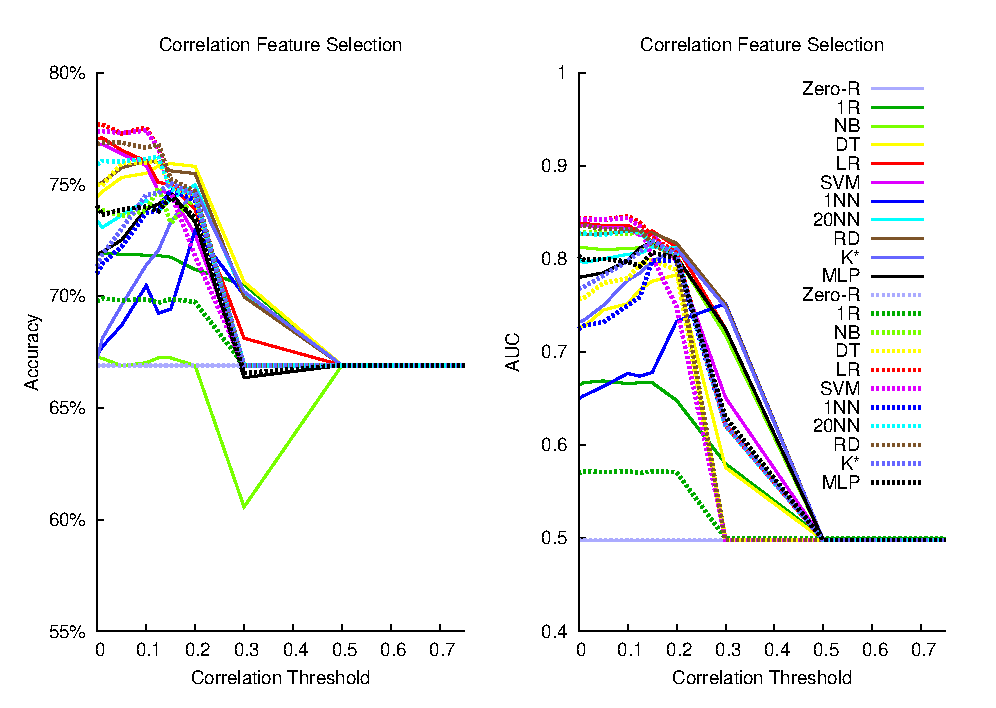
\includegraphics[width=\textwidth]{images/results/tr-corr.eps}
\caption{}
\label{fig:tr-threshold-corr}
\end{subfigure}
\caption{Comparison of accuracy and AUC between classifiers for feature selectors that discard features based on a threshold. Solid lines correspond to a result without discretisation, and dashed lines correspond to a result with discretisation.}
\label{fig:tr-threshold}
\end{figure}

\begin{figure}[htbp]
\ContinuedFloat
\begin{subfigure}{\textwidth}
\includegraphics[width=\textwidth]{images/results/tr-ig.eps}
\caption{}
\label{fig:tr-threshold-ig}
\end{subfigure}

\begin{subfigure}{\textwidth}
\includegraphics[width=\textwidth]{images/results/tr-oner.eps}
\caption{}
\label{fig:tr-threshold-oner}
\end{subfigure}
\caption{Comparison of accuracy and AUC between classifiers for feature selectors that discard features based on a threshold. Solid lines correspond to a result without discretisation, and dashed lines correspond to a result with discretisation.}
\end{figure}



In terms of classification accuracy, we did not find a lot of variation
between all classifiers, with Zero-R producing 66.91\% accuracy and 77.81\%
being the best we achieved -- an improvement of just over 10\%. The AUC of
the 11 classifiers we tested ranged from 0.498 with Zero-R to 0.846 with
logistic regression. Logistic regression, the \textit{de facto} method
used in LOS classification, performed consistently better than the others
across all feature
selection methods, but only when the feature set was not heavily reduced by
the feature selector: in these cases, such as the results from Figure
\ref{fig:tr-nothreshold-cfs-acc} showing classifier performance with features
selected by CFS, C4.5 decision trees and nearest
neighbour methods have higher accuracy than logistic regression. This is also
apparent from the graphs in Figure \ref{fig:tr-threshold}: for all three
feature selection methods, as we increase the threshold, logistic regression
drops in performance after the initial few thresholds and is outperformed by
C4.5 and the various nearest neighbour classifiers ($k$-NN with 1 and 20
neighbours, Ranked Distance and K*). This is true for both accuracy and AUC.

We found that in most cases, the SVM did not achieve a higher accuracy or
AUC than logistic regression with the same features even though SVMs are
considered the state-of-the-art in classification algorithms. Additionally,
as the feature set was reduced, the discriminating ability of SVMs (as
indicated by the AUC) decreased more than their accuracy: this is particularly
noticeable in Figure \ref{fig:tr-threshold-oner}, where the AUC of the SVM
drops sharply to below the AUC of even the 1R classifier at the 67.905\%
threshold, where there are
only 4 features. SVMs have not been used in a LOS classification problem like
ours, so there will need to be further work carried out in order to assess the
suitability of using SVMs to classify patient LOS.

Although the MLP has been investigated in studies attempting to identify
factors associated with longer LOS or mortality for trauma patients
\cite{Hunter2000,McGonigal1993}, leading to improved results with the neural
network, we did not see the MLP outperform all other classifiers with respect
to accuracy or AUC for any feature selection method for this data set. In fact,
the MLP often performed no better than any of the nearest neighbour
classifiers, which use a straightfoward mechanism of classifying unseen
examples. Even if the MLP had managed to achieve superior accuracy or AUC, the
``black box'' nature of its prediction decisions are a barrier for their
widespread use in medical decision-making.

Nearest neighbour approaches appear to have performed well on this data set in
both accuracy and AUC, especially in comparison to more sophisticated
classifiers and when the feature set is significantly reduced. From the graphs
in Figure \ref{fig:tr-threshold}, we can see that all the nearest neighbours
approaches perform similarly when the number of features is decreased, but our
Ranked Distance approach performs better than the other NN algorithms. This
improvement is not apparent at smaller feature sets, where using the standard
$k$-NN algorithm with 1 or 20 neighbours performs slightly better.
The performance of NN we observed in our results is
an interesting finding because nearest neighbours have not been commonly
applied in predicting the LOS, but there is intuitive appeal in the
case-by-case nature of how these algorithms classify new examples that should
be explored further. Unlike MLPs and SVMs, prediction decision of nearest
neighbours are more transparent and understandable. However, the major drawback
of NN algorithms is their storage requirement and the computational time
required to search for the nearest neighbours to make the classification.

There is a limitation to our findings that needs to be noted: we did not
attempt to tune the parameters of the classifiers in order to find the ones
that resulted in the best performance, so our statements are based on the
results of the default parameters of each classifier.
MLPs in particular are sensitive to
the network architecture, so it is likely that its accuracy and AUC could be
improved if the parameters were selected to optimise its performance on this
data set.

\subsection{General Data Set}
In Figures \ref{fig:pt-nothreshold} and \ref{fig:pt-threshold}, we compare the
performance of the classifiers we used on the general hospital data set. In
contrast to the trauma data, we were able to achieve very high accuracy and
AUC on this data set using the exact same classifiers and feature selection
methods. Instead of only a 10\% improvement from Zero-R by the best classifier
in the trauma data, we were able to achieve an accuracy of 98.23\%, which is
an increase of over 20\% from the Zero-R accuracy on this data set of 75.64\%.
Additionally, we also managed to observe very high ($>0.97$) AUC figures for
all classifiers except Zero-R and 1R.

\begin{figure}[htbp]
\begin{subfigure}{.48\textwidth}
\includegraphics[width=\textwidth]{images/results/pt-nofs-acc.eps}
\caption{}
\label{}
\end{subfigure}%
\begin{subfigure}{.55\textwidth}
\includegraphics[width=\textwidth]{images/results/pt-nofs-auc.eps}
\caption{}
\label{}
\end{subfigure}

\begin{subfigure}{.48\textwidth}
\includegraphics[width=\textwidth]{images/results/pt-cfs-acc.eps}
\caption{}
\label{}
\end{subfigure}%
\begin{subfigure}{.55\textwidth}
\includegraphics[width=\textwidth]{images/results/pt-cfs-auc.eps}
\caption{}
\label{}
\end{subfigure}

\begin{subfigure}{.48\textwidth}
\includegraphics[width=\textwidth]{images/results/pt-wrapper-acc.eps}
\caption{}
\label{}
\end{subfigure}%
\begin{subfigure}{.55\textwidth}
\includegraphics[width=\textwidth]{images/results/pt-wrapper-auc.eps}
\caption{}
\label{}
\end{subfigure}
\caption{Comparison of accuracy and AUC between classifiers for each non-threshold feature selection method, grouped by whether or not discretisation was applied.}
\label{fig:pt-nothreshold}
\end{figure}

\begin{figure}[htbp]
\begin{subfigure}{\textwidth}
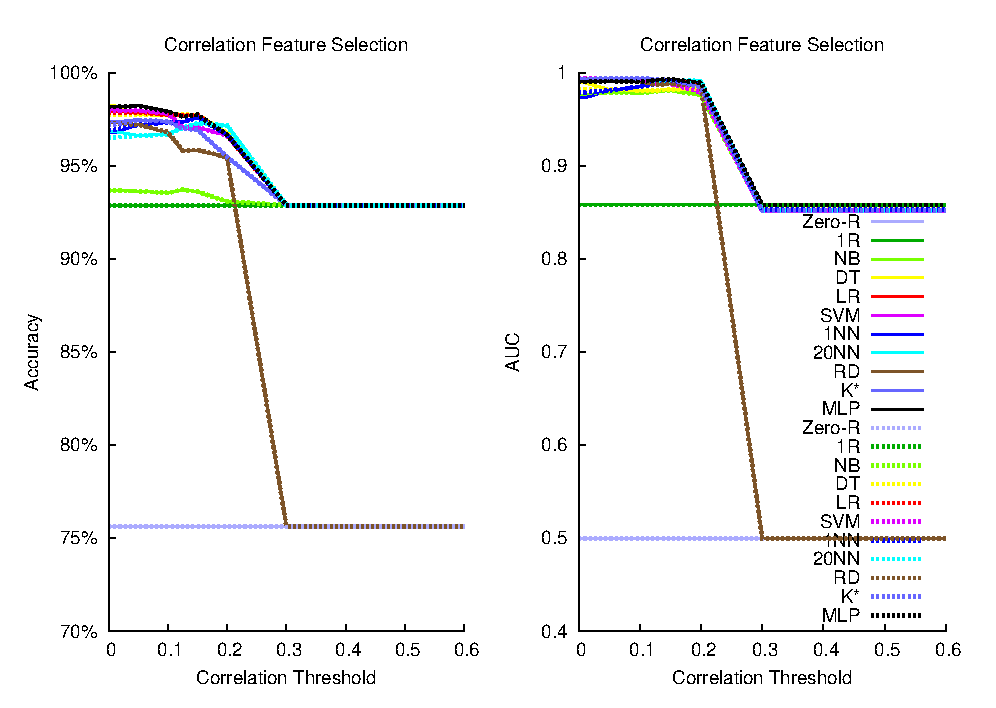
\includegraphics[width=\textwidth]{images/results/pt-corr.eps}
\caption{}
\label{fig:pt-threshold-corr}
\end{subfigure}
\ContinuedFloat
\begin{subfigure}{\textwidth}
\includegraphics[width=\textwidth]{images/results/pt-ig.eps}
\caption{}
\label{}
\end{subfigure}
\caption{Comparison of accuracy and AUC between classifiers for feature selectors that discard features based on a threshold. Solid lines correspond to a result without discretisation, and dashed lines correspond to a result with discretisation.}
\label{fig:pt-threshold}
\end{figure}

\begin{figure}[htbp]
\ContinuedFloat
\begin{subfigure}{\textwidth}
\includegraphics[width=\textwidth]{images/results/pt-oner.eps}
\caption{}
\label{}
\end{subfigure}
\caption[]{Comparison of accuracy and AUC between classifiers for feature selectors that discard features based on a threshold. Solid lines correspond to a result without discretisation, and dashed lines correspond to a result with discretisation.}
\end{figure}



Logistic regression and the SVM performed equal best in discriminating ability,
along with K* with an AUC of 0.994. We consider the performance of K* to be
superior because it was able to achieve this with 8 features out of 14, and
additionally it does not require any optimising of its parameters.
The AUC result of both logistic regression and the SVM were achieved with all
14 features. Although this is not a large number of features, simplifying the
inputs to a classifier is beneficial because it reduces the time needed for
training and classifying new examples. However, as indicated by the graphs in
Figure \ref{fig:pt-threshold} of AUC against threshold, and the bar charts in
Figure \ref{fig:pt-nothreshold}, the AUC of all classifiers except Zero-R and
1R was very close, around 0.98-0.99.

Notably, the MLP performed better than logistic regression on this data set
than on the trauma data, achieving better AUC with CFS and C4.5 wrapper feature
selection and better accuracy over all feature selection methods. This is a
surprising result as CFS and C4.5 wrapper select only 2 and 4 features
respectively. However, the major drawback of training the MLP with this data
set was the amount of time needed for one run of ten-fold cross-validation.
Even with only 14 features, the classifier required several hours to train.
Although we did not attempt to quantify the exact training time, it was by far
the slowest learning algorithm.
This is because the data set contained over 17000 training examples, which have
to be processed several times by the MLP until all of the weights between its
connections do not change more than a certain threshold.

Notice that in Figure \ref{fig:pt-threshold-corr}, both the accuracy and AUC
of Ranked Distance drop much more than for the other classifiers. This is at
a correlation coefficient threshold of 0.2, which reduces the feature set to
4 features. We noted in the discussion on classifiers for the trauma data set
that Ranked Distance performed worse for smaller feature sets than for larger
ones, and this is another example of this phenomenon. Recall that in Ranked
Distance, features are first ranked according to some similarity metric (we
have used the correlation coefficient), and then assigned a weight according
to their rank. The function we have used assigns rapidly decaying weights to
the features, which results in greater importance being placed on a few of
the features with the highest rank. Further work needs to be carried out to
investigate the cause of the poor performance on smaller feature sets, but
it is not altogether surprising: Ranked Distance performs best by using the
weighted distance contributions of all features, and by significantly reducing
their number we can expect to sharply reduce its ability to differentiate
between neighbours. There is also scope for investigating other weight
assignment functions which would work better in reduced-feature situations.

\section{Effect of Discretisation}
We touched briefly upon the effect of discretisation on the performance of the
classifiers used, but we would like to point out a few other things not
mentioned earlier. Firstly,
although discretisation improved the best accuracy and AUC for many
classifiers trained on the trauma data, this was only when using a larger
proportion of features: note the dotted lines in
Figures \ref{fig:tr-threshold-corr}, \ref{fig:tr-threshold-ig} and
\ref{fig:tr-threshold-oner} are above their solid line counterparts of the
same colour on the very left of the graph (where no features have been
discarded), but as we increase the threshold and more features are discarded,
the classifier using the discretised data set does not always perform better.
Notably, discretisation improves the accuracy and AUC of nearest neighbour
classifiers when few features have been removed, but as the number of features
decreases, these approaches perform worse with discretised features.

Although the results from discretisation with varying thresholds of the
correlation, information gain and 1R feature selectors are mixed, the graphs
in Figure \ref{fig:tr-nothreshold} show improvements in AUC and accuracy for
most classifiers in most of the situations, and show that discretisation is a
viable pre-processing technique for data mining problem. This improvement is
not present in the general hospital data set due to the nature of the data set:
as mentioned earlier, only one feature is discretised, which transforms it into
a single value. This single value does not help the classifier distinguish
between classes, and hence degrades performance.

Discretisation consistently improved the accuracy and AUC of the Na\"{i}ve
Bayes classifier, which suggests that it is more suitable for the data than the
classifier's assumption that continuous-valued features follow a normal
distribution.

Supervised discretisation such as the one we have used is very specific to the
data set, so it is difficult to draw general conclusions that will apply to
other learning problems. However, we have not yet seen this technique being
used in LOS prediction problems, and we believe it is worth investigating
when approaching a new learning problem.

\section{Summary}
In this section we have presented and discussed the main findings of our
work, examining the overall picture, and then detailing comparisons between
classifiers and feature selection methods in detail before concluding with a
few remarks on discretisation.

We found that irrespective of discretisation or feature selection, logistic
regression still performed better than other learning algorithms, which
reaffirms its use as the \textit{de facto} classifier in predictive medicine.
However, we were also able to achieve results that were almost as good using
nearest neighbour approaches combined with feature selection techniques,
neither of which have been investigated thoroughly in previous work. Our
proposed Ranked Distance approach was able to improve the accuracy and AUC of
the standard $k$-NN algorithm with the same number of neighbours, but we found
that its performance suffered when used in conjunction with feature selection.

In both the trauma and general hospital data sets, we were not able to
consistently improve the accuracy and AUC of all
classifiers with feature selection but we were able to sacrifice some
predictive power in order to use a drastically reduced feature set: for trauma
we found that K* with 11 features selected by a C4.5 wrapper performed only
slightly worse in discriminating between the two LOS classes than logistic
regression using 29 features, and for the hospital-wide data we achieved
0.983 AUC using only 2 features out of 14 using the MLP, 0.011 less than the
best result from logistic regression which required all 14 features. It is
therefore important to consider the trade-off between predictive ability,
speed and ease of understanding when making judgements about classifiers.

Finally, we pointed out that although discretisation was able to improve
classifier performance, this effect was less noticeable when more features
were discarded from feature selection. Discretisation has not been used
extensively in the LOS prediction literature, so our work will serve as a
starting point for further investigation.

\chapter{Conclusions and Future Work} \label{chap:conclusion}

In this thesis we conducted a systematic and empirical evaluation of a number
of classification algorithms and feature selection methods, as well as the
effect of discretisation, for predicting the length of hospital stay of trauma
patients. In particular, we introduced a new classification algorithm, Ranked
Distance Nearest Neighbour, and compared its accuracy and AUC with ten
other classifiers -- Zero-R, 1R, Na\"{i}ve Bayes, C4.5 decision tree, logistic
regression, support vector machine, $k$-nearest neighbour with $k=1$ and 20,
K* and multi-layer perceptron -- several of which (for example K*) have not
been used in existing work on LOS prediction. We also investigated a variety of
feature selection methods -- CFS, C4.5 wrapper, correlation coefficient,
information gain, 1R and expert selection -- encompassing both manual and
automatic methods, many of which have not been applied to the problem of LOS
prediction. Our experiments were conducted on two data sets, one from the
trauma ward of a Sydney hospital and the other a general hospital-wide data
set from Portugal.

\section{Conclusions}
The best accuracy we achieved on the trauma data was 77.81\% with the $k$-NN
classifier using 1 nearest neighbour and 11 out of 78 features. This represents
an improvement over previous work done by Dinh et al. \cite{Dinh2013a}
on the same data set,
where they managed to achieve 75.06\% with logistic regression. More
importantly, we were able to improve upon their AUC of 0.812 with a result of
0.846, also using logistic regression but first discretising numeric features
and reducing the feature set to 29 features.
If we consider an even smaller number of features, then K*
gives an AUC of 0.838 with 11 features selected by the C4.5 wrapper, which
improves upon the result of Dinh et al. \cite{Dinh2013a} while using a little
more than half
the number of features. The drawback of $k$-NN and K* is that they require all
examples to be stored and then searched during classification, which becomes
storage- and computation-expensive as the data set increases in size.

We were able to achieve substantially better results on the hospital-wide data,
with a best accuracy of 98.23\% using a C4.5 decision tree and best AUC of
0.994 achieved equally by logistic regression, SVM and K*. Like with the
trauma data, we were also able to sacrifice a small amount of accuracy or AUC
in order to use substantially less features: the MLP was able to achieve
96.45\% accuracy and 0.983 AUC while using only 2 out of 14 features. In both
these data sets, investigating feature selection was not only a way to
improve the performance of our classifiers, but also allowed us to see the
trade-off between the two (sometimes conflicting) objectives of increasing
predictive power and reducing feature set size.

An important contribution of our work is the use of several nearest neighbour
algorithms for predicting the LOS class of a patient. We found that these
techniques can achieve good accuracy and discriminating ability if a suitable
set of features is found. In addition, we proposed a new algorithm, Ranked
Distance Nearest Neighbours, which is an extension of the standard nearest
neighbours classifier that takes the relative importance
of each feature into account when determining the nearest neighbours of an
example. We found that this achieved better results than the other nearest
neighbour algorithms we evaluated, but only when most of the original feature
set was used.

Although we were able to improve on the work of Dinh et al. \cite{Dinh2013a}
and confirm the
importance of some features they and others found in predicting the LOS for
trauma patients, we did not find a single classifier or feature selector
that was superior to the others but instead observed different combinations
giving better results than others in certain situations. This highlights the
importance of understanding the data and investigating a range of classifiers
and feature selection techniques when approaching any medical data mining
problem, for which our work will become a catalogue.
However, we did find that logistic regression tended to perform well
on both data sets and across a number of feature selection methods, supporting
its common use in deriving classifiers for various medical phenomena.

\section{Future Work}
In this thesis we have systematically evaluated a large number of combinations
of classifiers and feature selection methods while also testing the effect of
supervised discretisation, and have thus created a catalogue of examples of
the application of data mining techniques to LOS classification. Our work on
this topic has raised a number of avenues for futher research, one of which is
to re-formulate the binary classification problem as a \textit{multi-class}
classification problem. Our current categorisation of the LOS outcome is very
crude: we can only classify patients into two categories. In order to better
assist physicians in making decisions, we could split the classification into
three or more classes, such as 1-3 days, 4-10 days and $>$11 days, and
investigate how different classifiers and features perform for this slightly
different problem.

We mentioned in the discussion in Chapter \ref{chap:results} that we did not
fine-tune the parameters of the classifiers that we evaluated. There is room
for us to optimise these parameters and test whether these result in
significant improvements in accuracy and AUC, and explore reasons why this
did or did not help. We could also broaden our investigation by additionally
using another data set, preferably from a different medical domain.

In our proposed Ranked Distance Nearest Neighbour algorithm, we only considered
one kind of weight assignment function, but it is not the only way to assign
these weights. There is room to investigate other types of functions, as well
as using weights obtained from another algorithm (such as logistic regression).
In addition to assigning the weights, we have also only investigated one method
of determining the relative importance of features: the correlation coefficient.
This leaves much room to use other ways of ranking features, such as the
information gain and 1R accuracy (which we have used in our work as feature
selectors).

Another area of potential future work is to investigate \textit{ensembles} of
classifiers, which take the predictions of more than one classifier (of the
same or different kind) and combine them to make a final prediction. There are
numerous ways in which this can be done: an example is to take the majority
class that is predicted as the final prediction for our ensemble. Ensembles
have often been demonstrated to perform better than any single classifier,
and there is a wide range of methods and combinations we could evaluate in
order to assess their performance relative to the single classifiers we have
used in our work.



%%%%%%%%%%%%
% End

% Bibliography
%\bibliographystyle{style/mybibstyle}
\bibliographystyle{abbrv}
{
\setstretch{1.25}
\cleardoublepage
\phantomsection
\bibliography{references}
}

%%%% Appendices
\appendix
\addtocontents{toc}{\protect\setcounter{tocdepth}{1}}
\documentclass{article}

\usepackage{amsfonts}
\usepackage{amsmath}
\usepackage{amsthm}
\usepackage{graphicx}
\usepackage[colorlinks=true,citecolor=blue,linkcolor=blue,filecolor=blue,urlcolor=blue,pdfborder={0 0 0}]{hyperref}
\usepackage[utf8]{inputenc}
\usepackage{multicol}
\usepackage{natbib}
\usepackage{subcaption}

\title{Nearest Neighbour Methods for Length of Stay Prediction}
\author{
  Tianyu Pu, Irena Koprinska, Kalina Yacef\\
  School of Information Technologies\\
  University of Sydney, NSW, 2006\\
  \texttt{\{tianyu.pu,irena.koprinska,kalina.yacef\}@sydney.edu.au}
  \and
  Michael Dinh\\
  Trauma Services, Royal Prince Alfred Hospital\\
  Sydney, NSW, 2042\\
  \texttt{dinh.mm@gmail.com}
}

\date{\today}

\begin{document}
\maketitle

\renewcommand{\abstractname}{Summary}

\begin{abstract}
Objective:

Materials and methods:

Results:

Conclusions:

Keywords:

\end{abstract}

\section{Introduction}
Hospitals often have limited funding, and therefore managing and utilising
their resources efficiently has always been a priority \cite{Walczak2003}.
One key measurement of hospital activity, health care utilisation and hospital
cost is the patient length of stay \citep{Omachonu2004,Ng2006}.
The length of
stay has been used in a wide variety of medical domains, such as burns
 \citep{Yang2010}, intensive
care \citep{Tu1993,Harper2005,Perez2006,Dybowski1996},
psychiatry \citep{Lowell1997}, and acute pancreatitis \citep{Pofahl1998}, in
order to assist hospitals in allocating beds and other patient management
resources as efficiently as possible. However, given the many different
conditions that hospitals manage, the length of stay of a patient is
not easy to predict \citep{Walczak2003}, especially upon a patient's admission.
Many methods have been explored in the literature, from the realm of statistics
to techniques in data mining, and they have been explored for many different
medical domains.

One of the more well-understood and widely used statistical methods for
predicting the length of stay is \textit{logistic regression} \citep{Tu1996}.
Logistic regression models are straightforward to construct and use via the
help of statistical software packages such as
SAS\footnote{SAS Institute, Cary, NC, USA}, and
also make the contribution of each independent variable to the final
prediction explicit. Thus they are easier to interpret when compared to more
``black box'' approaches such as artificial neural networks \citep{Adams2012}.
A wide variety of other statistical approaches have been proposed, notably:
various scoring systems from univariate analysis \citep{Adams2012,Lavoie2005},
linear regression \citep{Yang2010}, exponential models \citep{Clark2007},
survival analysis \citep{Vasilakis2005}, and Markov
models \citep{Perez2006,Jain1989,Kapadia2000}.

Out of the development of the various statistically-motivated models, data
mining techniques, particularly artificial neural networks,
began to be more widely adopted following a number of
early applications to length of stay prediction in intensive
care \citep{Tu1993,Dybowski1996}, in addition to disease diagnosis and mortality
prediction \citep{Silva2006}. Artificial neural networks are able to detect
complex and non-linear relationships between input and output variables and can
be developed using many different techniques. Much work has been done in using
neural networks to predict patient length of stay in various medical conditions
such as acute pancreatitis \citep{Walczak2003}, gastroenteritis \citep{Ng2006},
surgical intensive care \citep{Buchman1994,Tu1993} and
psychiatry \citep{Lowell1997}. Other data mining techniques have also been
applied, such as support vector machines and tree-based
methods \citep{Harper2005}.

One of the major drawbacks of sophisticated data mining techniques is the high
level of difficulty required in interpreting their predictions and the factors
affecting those predictions. This is
particularly true of artificial neural networks and the state-of-the-art
support vector machine, which are able to achieve very high accuracy but can be
non-intuitive to understand. Medical domain experts who use the predictions of
trained learning algorithms need to understand how the algorithm reached its
decision before they are able to confidently use it to aid their clinical
decision-making.

In this paper we present the application of nearest neighbour methods
in predicting the length of stay category for patients admitted to a trauma
ward. The categories are \textit{less than or equal to 2 days} or
\textit{greater than 2 days}, which have been used in previous work on length
of stay prediction in the same medical domain \citep{Dinh2013a}.
Nearest neighour methods have not been studied in predicting the length of stay,
and we believe they are much more intuitive to
understand than techniques such as support vector machines.
Additionally, they can be adjusted to suit particular medical domains by
changing their similarity function. We compare the performance of the basic
nearest neighbour algorithm, as well as an extension (K*), against the
performance
of previous work which used logistic regression. We also propose a novel
extension to the standard nearest neighbour algorithm, Ranked Distance, and
test its performance against the other classifiers. In addition, we apply a
range of feature selection methods and systematically investigate the effect
of discretisation, as they have not been
thoroughly studied in existing work. Finally, we compare the performance of
these with the state-of-the-art support vector machines and the
commonly-used artificial neural networks.

We found that the standard nearest neighbour classifier using only 1 nearest
neighbour achieved a ten-fold cross-validated accuracy of 77.81\%, the highest
out of all the methods. This is an improvement of 2.75\% over previous work
carried out by Dinh et al. \citep{Dinh2013a} using the same data set. Also, the
nearest neighbour classifiers almost always outperformed the logistic
regression, support vector machines and neural networks when the number of
features was gradually reduced. This means that predictions are able to be made
more quickly, and will also be more intuitive to interpret and understand for
physicians.

In Section \ref{sec:nn}, we outline the basics of nearest neighbour
classification and describe both the existing K* extension and our proposed
extension, Ranked Distance. Section \ref{sec:features} outlines the feature
selection methods we used. Section \ref{sec:eval} describes the method used
to evaluate the performance of these classifiers, and Section \ref{sec:results}
proceeds to discuss the results. We present concluding remarks in Section
\ref{sec:conclusions}.

\section{Nearest Neighbour Classification}
\label{sec:nn}

\subsection{Basic Algorithm}
The $k$-nearest neighbour ($k$-NN) classifier is an example of an
\textit{instance-based} learning algorithm. This is because it does not attempt
to deduce or
generalise a relationship between the features and the class: it simply stores
all training examples and classifies an unseen example by finding the $k$
``nearest'' examples (or \textit{instances}) and assigning the majority class
to the new example. In the simplest form of the algorithm, $k$ is chosen to be
1 and the Euclidean distance is used to measure the closeness of neighbours:
\begin{equation*}
\mathrm{Distance} = \sqrt{(x_1-y_1)^2 + (x_2-y_2)^2 + \ldots + (x_n-y_n)^2}
\end{equation*}
where $x_i,y_i$ are the values of the $i$-th feature for two different feature
vectors (or instances).

$k$-NN allows all features to be taken
into account equally when classifying a new example. However, since feature
values often span different ranges and units of measurement, a particularly
large range of values for a feature would contribute much more to the distance
than another feature that spans a lower set of values.
To avoid this, it is important to \textit{normalise} the
values of each numeric feature before using $k$-NN: for each feature $i$, we
calculate the normalised value of the feature for each training example. This
is done using the following relationship:
\begin{equation}
\label{eq:normalise}
a_i = s\left(\dfrac{v_i - \mathrm{min }v_i}{\mathrm{max }v_i - \mathrm{min }v_i}\right) + t
\end{equation}
where $a_i$ is the normalised feature value, $v_i$ is the actual value in the
data set, max $v_i$ and min $v_i$ are taken over all training examples, $s$ is
a scaling factor and $t$ indicates how much to translate the range by. If $s=1$
and $t=0$, then the range of normalised values will be in $[0,1]$.

\subsection{Existing and Proposed Extensions}
There have been many extensions proposed to the $k$-NN algorithm described
above. These usually seek to find a more suitable distance metric for the
problem domain at hand, or to reduce the storage requirements of the original
$k$-NN algorithm (since the classifier makes no attempt to generalise from the
examples, all of them must be stored).
We will focus on two algorithms that extend the standard Euclidean distance:
K* and our proposed approach, Ranked Distance Nearest Neighbour.

\subsubsection{K*: Instance-based Classifier with Entropic Distance Function}
Cleary and Trigg developed K*, an instance-based classifier that uses entropy
to measure the distances between instances \cite{Cleary1995}. They consider
the distance between two instances to be the complexity of transforming one
into another. Define a sequence of transformations on an instance:
\begin{equation*}
\bar{t}(a) = t_n(t_{n-1}(\ldots t_1(a)\ldots)), \bar{t} \in T
\end{equation*}
where $\bar{t} = t_1,\ldots,t_n$. We can define a probability function $p$
that gives the probabilities of these transformations occurring, and then we
can define a probability function that gives the probabilities of all paths
(transformations) from example $a$ to $b$:
\begin{equation*}
P^*(b|a) = \sum_{\bar{t}\in T:\bar{t}(a)=b} p(\bar{t})
\end{equation*}
Within this framework, we can define transformations for both real-valued and
categorical features, which allows K* to work with all types of features.
The K* function is then defined as:
\begin{equation*}
K^*(b|a) = -\mathrm{log}_2P^*(b|a)
\end{equation*}

To calculate the probability of an instance $a$ being in a class $C$, we sum
the probabilities from $a$ to each instance of $C$, and repeat for each class.
The predicted class will be the one with the highest probability:
\begin{equation*}
P^*(C|a) = \sum_{b\in C} P^*(b|a)
\end{equation*}

We use K* as a comparison to the basic NN algorithm and also as a comparison
to our proposed Ranked Distance Nearest Neighbour algorithm. Additionally,
K* has not been yet been applied in predicting LOS, and its performance in this
domain is worth investigating.

\subsubsection{Ranked Distance Nearest Neighbour}
\paragraph{Intuition}
As we mentioned earlier, all features are considered equally in a $k$-NN
classifier, which implies that all features are equally important in predicting
the class. In practice, however, this is not always the case: to predict the
LOS of a trauma patient, the severity of their injury should affect the final
LOS more than whether or not they can speak English (which could be just two
of many features that are recorded about a patient). Our contribution is a
new NN algorithm that uses a modified distance function which takes into
account the relative importance of all features called Ranked Distance
Nearest Neighbour (RD).

\paragraph{Mathematical formulation}
Given two instances $\mathbf{x} = (x_1,x_2,\ldots,x_n)$ and
$\mathbf{y} = (y_1,y_2,\ldots,y_n)$, the distance between them is given by:
\begin{equation*}
\mathrm{Distance} = \sum_{i=1}^n w_i |x_i-y_i|
\end{equation*}
where the $w_i$s weight the contribution of the $i$-th feature to the overall
distance that is computed by the $k$-NN algorithm. We assume that all feature
values have been normalised, as described above.

\paragraph{Assignment of weights}
The weights $w_i$ can be tuned to match the particular problem that is being
investigated. For our LOS classification problem, we will consider one way
of weighting features.
First, we compute the correlation coefficients as described in the point above.
This gives us a ranking of the importance of each feature to the prediction of
the class, with 1 being the highest rank (indicating the most importance) and
$n$ being the lowest rank (indicating the least importance).
Instead of using the values of the correlation directly to weight
the distance contribution of each feature, we specify a function:
\begin{equation*}
f : \mathrm{Rank} \rightarrow \mathbb{R}, \mathrm{Rank} \in \{1,2,\ldots,n\}
\end{equation*}
that describes
how the weights of the features vary with the rank. This function should
inituitively be non-increasing and should produce lower values when the rank
number is greater, meaning that less important features have a lower weight
in the distance calculation.
Note that choosing $f(\mathrm{Rank}) = k$ for any non-zero constant $k$
results in all features contributing equally to the distance calculation.
We will use $f(\mathrm{Rank}) = \frac{1}{\mathrm{Rank}^c}$, where
$c$ varies from 0 to 1.

\section{Feature Selection}
\label{sec:features}
Here we introduce the feature selection algorithms we evaluate in our work.
Several of these have not been investigated in previous work on LOS prediction.
The role of feature selection is to reduce the number of attributes taken into
consideration by a learning algorithm, which improves running speed and can
make the resulting learned relationship easier to understand. We used both
automatic and manual methods of selecting features.

\subsection{Automatic Selection}
Automatic feature selection involves calculating the ``relevance'' of each
feature to predicting the class and only keeping features for use in training
if their relevance is above some threshold. We consider the Pearson correlation
coefficient, information gain and the wrapper approach.

\subsubsection{Pearson Correlation Coefficient}
The Pearson correlation coefficient measures the degree of linear correlation
between two variables. It is always in the range $[-1,1]$, where $-1$ is total
negative correlation, 0 is no (linear) correlation, and 1 is total positive
correlation. We compute the Pearson correlation between each feature and the
class using:
\begin{equation*}
r_i = \dfrac{\sum_{i=1}^m (x_i-\bar{x})(c-\bar{c})}{\sqrt{(\sum_{i=1}^m x_i-\bar{x})(\sum_{i=1}^m c-\bar{c})}}
\end{equation*}
where $m$ is the number of training examples, $x_i$ is the value of feature
$i$, and $\bar{x}$ and $\bar{c}$ are the arithmetic averages of the feature
values and the class values respectively.

\subsubsection{Information Gain}
We can also measure the information gain (IG) of each feature as follows.
If we have a class $C$ and a feature $F$, the entropy of the
class before and after observing the feature is:
\begin{equation*}
\begin{aligned}
& \mathrm{entropy}(C) = - \sum_{c \in C} p(c) \mathrm{log}_2 p(c) \\
& \mathrm{entropy}(C|F) = - \sum_{f \in F} p(f) \sum_{c \in C} p(c|f) \mathrm{log}_2 p(c|f)
\end{aligned}
\end{equation*}
The decrease in entropy reflects the gain in information provided by the
feature and is given by:
\begin{equation*}
IG(C|F) = \mathrm{entropy}(C) - \mathrm{entropy}(C|F)
\end{equation*}

We can compute the IG for each feature and then select subsets of features that
are greater than some threshold we specify, similar to the correlation
coefficient method of feature selection. We choose a similar set of thresholds
because of the high numbers of features with very low information gain.

\subsubsection{Wrapper-based Feature Selection}
The feature selection methods described above (Pearson correlation and IG) have
been described as \textit{filter} approaches to
attribute selection, because the feature set is reduced \textit{before} it
is given to the learning algorithm.
Kohavi and John proposed another approach, the \textit{wrapper} approach:
instead of performing feature selection independently of the learning
algorithm using some measure of ``relevance,''
the learning algorithm itself is used to evaluate the goodness of
subsets of features \cite{Kohavi1997}. 

A key advantage of the wrapper approach is that the selected feature sets are
specifically tailored to a learning algorithm, which ensures the best
performance of that algorithm given the data set. However, wrapper approaches
can also be prohibitively slow if the data or feature sets are large and the
chosen learning algorithm expensive to train (such as support vector machines
and multi-layer perceptrons). We will evaluate the use of C4.5 decision trees
in selecting features using the wrapper approach.
Using decision trees to select features is relatively fast as due to the
divide and conquer nature of the learning algorithm, and the tendency of the
trees to select fewer features for learning than other algorithms.
Wrapper methods search for the best subset of features and do not require a
threshold to discard attributes.

\subsection{Manual Selection}
All of the above automatic feature selection methods use some notion of
``relevance,'' such as information gain or linear correlation,
in order to determine the best subset of features to select.
Depending on the problem at hand, these definitions of relevance may or may
not work well with the data. In the LOS prediction literature, studies
have enlisted the help of medical domain experts to assist in feature
selection, due to their experience and understanding of the underlying
problem and the effect of the features on the outcome. It will therefore be
worthwhile to compare the performance of classifiers using features selected
automatically and manually.

\subsubsection{Domain Expert Selection}
Consultation with a domain expert yielded a feature set that we
use to compare with the baseline and with the other automatic methods.

\subsection{Baseline Feature Set}
The key previous work on trauma LOS prediction was by Dinh et. al.
\cite{Dinh2013a}, who used a specific feature set from the data set that we
use. We would like to use the features they selected as a baseline for
evaluating the other feature selection methods we describe.

\section{Evaluation}
\label{sec:eval}
\subsection{Data Set}
The data set used consisted of trauma registry data from the trauma centre
at the Royal Prince Alfred Hospital, a major trauma centre in New South Wales,
Australia. It covered all adult (age 15 and over) inpatient admissions to the
trauma centre from 2007--2011. 
All patients were first admitted to the trauma ward until discharged
or transferred to an appropriate unit within the hospital. A single trained
data manager recorded a variety of attributes about the admitted patient,
such as age, gender, blood pressure, mechanism of injury and body regions
that were injured.

There were 2546 patient records in the data set we received, comprising of 79
features, one of which was the target variable \texttt{los48}.
\texttt{los48} was a binary variable -- that is, it could only take two
values, 0 or 1 -- with 1 indicating that the patient stayed two days or less,
and 0 indicating a stay of longer than 2 days.

\subsection{Preprocessing}
The data set was cleaned by correcting spelling and punctuation
inconsistencies and removing extraneous whitespace. Examples which had missing
values for at least one feature were removed, in line with previous work on the
same data set.

Continuous-valued features were then normalised into the $[0,1]$ range as
described in Section \ref{sec:nn} above, substituting $s=2$ and $t=-1$ into
Equation \ref{eq:normalise}. These continuous features were then discretised
using Fayyad and Irani's method of supervised discretisation
\citep{Fayyad1993}. We kept both the original data set (normalised, without
discretisation) and the discretised (and normalised) data set for comparison.

\subsection{Classification Algorithms}
We tested the performance of
support vector machines (SVMs), multi-layer perceptrons (MLPs), $k$-nearest
neighbour with 1
and 20 nearest neighbours, K* and logistic regression (LR), as well as our
proposed
Ranked Distance Nearest Neighbour (RD) -- a total of 7 different classifiers.

\subsection{Statistical Significance}

\subsection{Experimental Setup and Procedure}
The steps that we took to evaluate the performance of the various classifiers
and feature selection methods were:
\begin{enumerate}
\item For both the discretised and non-discretised data set, we trained all 7
classifiers without feature selection. Evaluation was performed using ten runs
of \textit{ten-fold stratified cross-validation}.
\item Then, for each data set, we evaluated the effect of the 3 automatic
feature
selection methods on each of the 7 classifiers listed above, giving us 21
configurations for the discretised and non-discretised data set.
\item In order to ensure that the baseline in the literature was comparable
to our work, we used the baseline features and applied their method, logistic
regression, to obtain a measure of performance on the non-discretised data set.
We also evaluated this feature set against the rest of the 6 classifiers, and
repeated this using the discretised data.
\item Additionally, the expert-selected features were tested against all 7
classifiers, with both the discretised and non-discretised data.
\end{enumerate}

\section{Results and Discussion}
\label{sec:results}

\subsection{Overall Performance}
The best accuracy was 77.81\%, achieved using the $k$-NN algorithm
with 1 nearest neighbour, a discretised data set, and feature selection using a
C4.5 wrapper. The best AUC of 0.846 was achieved using logistic regression with
features selected by a correlation coefficient threshold of 0.1, again
using the discretised data set.

\begin{figure*}[htbp]
\begin{subfigure}{.48\textwidth}
\includegraphics[width=\textwidth]{../thesis/images/results/tr-nofs-acc.eps}
\caption{}
\label{}
\end{subfigure}%
\begin{subfigure}{.55\textwidth}
\includegraphics[width=\textwidth]{../thesis/images/results/tr-nofs-auc.eps}
\caption{}
\label{}
\end{subfigure}

\begin{subfigure}{.48\textwidth}
\includegraphics[width=\textwidth]{../thesis/images/results/tr-dinh-acc.eps}
\caption{}
\label{}
\end{subfigure}%
\begin{subfigure}{.55\textwidth}
\includegraphics[width=\textwidth]{../thesis/images/results/tr-dinh-auc.eps}
\caption{}
\label{}
\end{subfigure}

\begin{subfigure}{.48\textwidth}
\includegraphics[width=\textwidth]{../thesis/images/results/tr-expert-acc.eps}
\caption{}
\label{}
\end{subfigure}%
\begin{subfigure}{.55\textwidth}
\includegraphics[width=\textwidth]{../thesis/images/results/tr-expert-auc.eps}
\caption{}
\label{}
\end{subfigure}

\begin{subfigure}{.48\textwidth}
\includegraphics[width=\textwidth]{../thesis/images/results/tr-wrapper-acc.eps}
\caption{}
\label{}
\end{subfigure}%
\begin{subfigure}{.55\textwidth}
\includegraphics[width=\textwidth]{../thesis/images/results/tr-wrapper-auc.eps}
\caption{}
\label{}
\end{subfigure}
\caption[]{Comparison of accuracy and AUC between classifiers for each non-threshold feature selection method, grouped by whether or not discretisation was applied.}
\label{}
\end{figure*}

Recall that in order for our work to be comparable to that of previous work on
trauma LOS prediction by Dinh et al. \cite{Dinh2013a}, we use the same data
set and also test the features they used as the baseline feature set.
From Table \ref{tab:overall-tr-acc} we can see that
the best accuracy achieved using their features is 75.06\% with logistic
regression.
It is worth noting that our best accuracy, using $k$-NN with 1
nearest neighbour, shows a statistically significant improvement of 2.75\% upon
the accuracy achieved by Dinh et al.
while using only 11 features (compared to the 19 they used). These 11 features
make up only 14.1\% of all features in the data set, and performed better than
the 11 features selected manually by the domain expert.

Despite our inclusion of accuracy as an evaluation metric, the AUC is what Dinh
et al. \cite{Dinh2013a}
used to evaluate the ability of their logistic regression classifier to
discriminate between the two LOS classes. Using their features, the best AUC
was 0.812 with logistic regression, and our best result was 0.846, also with
logistic regression. However, this was using the discretised data set with 29
features selected by correlation coefficient at a threshold of 0.1.
Although our logistic regression classifier exhibited an AUC improvement of
0.034, it required roughly 50\% more features than the baseline of 19 features.
If we are willing to sacrifice a little discriminating power, we are able to
achieve 0.838 AUC with only 11 features using the K* classifier.

Although $k$-NN with 1 nearest neighbour had the highest accuracy (77.81\%) out
of all combinations of classifiers and feature selection methods for this data
set, we should mention that logistic regression came a very close second with
77.7\%, outperforming more sophisticated approaches such as SVM and MLP. It
also achieved a higher AUC, and has the added advantages of being faster to
train and widely applied in medicine.

\subsection{Comparison of Feature Selection Methods}
The best accuracy and AUC results for
each classifier resulted from a reduced feature set obtained through a
particular feature selection method. Out of 20 combinations of classifiers
and discretisation (the 10 classifiers with and 10 without
discretisation), the C4.5 wrapper method resulted in the best
accuracy for 7 of these combinations, followed by 5 using information gain
and 4 using the correlation coefficient and very few for the other methods.
\texttt{TODO: recount the numbers in this paragraph.}

In terms of AUC, we
find that the correlation coefficient and the information gain are the feature
selectors that give the best AUC for most of the classifiers, and perform
equally well when used in conjunction with logistic regression and SVMs.
Interestingly, although the C4.5
wrapper method selects features which allow classifiers to achieve good
accuracy, only in 2 out of the 20 combinations of classifiers did it give the
best AUC result out of all the feature selectors.

Note that regardless of whether we consider accuracy or AUC to be more
important in evaluating classifiers, neither the baseline
feature set from Dinh et al. \cite{Dinh2013a} nor the features suggested by
the expert yielded better
results than automatic feature selection in all but \texttt{two?} cases. Neither
feature selection method produced the best AUC result for any classifier.
This is a surprising result because intuitively -- and in the literature -- it
has been stated that in a highly specialised field such as medicine, the domain
experts would be best-equipped to make judgements about which features to
use \cite{Witten2005}, and these should give reasonable results. However,
our results show that in attempting to classify patients according to their
LOS, we should consider both manual and automatic approaches.

Recall that $k$-NN with 1 nearest neighbour and C4.5 wrapper feature
selection produced the best accuracy (77.81\%) for the data set, and
logistic regression with correlation coefficient feature selection at a
threshold of 0.1 gave the best AUC (0.846). These two feature selection
methods selected 11 and 29 features respectively, and the features that
were chosen in common between them were: \texttt{operation}, \texttt{bp},
\texttt{iss}, \texttt{lowerlimbnopelvis}, \texttt{age}, \texttt{lowerlimbany}
and \texttt{icu}. This adds evidence to the work of Dinh et al. who found
that \texttt{iss}, \texttt{age} and \texttt{operation} were important
distinguishers of LOS $\leq$ or $>$ 2 days \cite{Dinh2013a}. We also
confirm the findings of Gabbe et al. who found that \texttt{age},
\texttt{iss} and \texttt{bp} were useful in predicting the length of
hospital stay of blunt trauma patients \cite{Gabbe2005}. Our feature
selection results also
support the findings of McGonigal et al. \cite{McGonigal1993} who used
\texttt{age} and
\texttt{iss} to predict the probability of survival for trauma patients, a
related problem in the same medical domain.
Our observations suggest the use of feature selection not only as a
pre-processing step to improve the accuracy or AUC of a classifier, but also
as a tool used independently to extract insights from medical data.

\subsection{Comparison of Classifiers}
In terms of classification accuracy, we did not find a lot of variation
between all classifiers, with Zero-R producing 66.91\% accuracy and 77.81\%
being the best we achieved -- an improvement of just over 10\%. The AUC of
the 11 classifiers we tested ranged from 0.498 with Zero-R to 0.846 with
logistic regression. Logistic regression, the \textit{de facto} method
used in LOS classification, performed consistently better than the others
across all feature
selection methods, but only when the feature set was not heavily reduced by
the feature selector: in these cases, such as the results from Figure
\ref{fig:tr-nothreshold-cfs-acc} showing classifier performance with features
selected by C4.5 and nearest
neighbour methods have higher accuracy than logistic regression. This is also
apparent from the graphs in Figure \ref{fig:tr-threshold}: for both
feature selection methods, as we increase the threshold, logistic regression
drops in performance after the initial few thresholds and is outperformed by
C4.5 and the various nearest neighbour classifiers ($k$-NN with 1 and 20
neighbours and K*), as well as our Ranked Distance algorithm.
This is true for both accuracy and AUC.

We found that in most cases, the SVM did not achieve a higher accuracy or
AUC than logistic regression with the same features even though SVMs are
considered the state-of-the-art in classification algorithms. Additionally,
as the feature set was reduced, both the discriminating ability of SVMs
(indicated by the AUC) and accuracy decreased noticeably. SVMs have not been
used in a LOS classification problem like
ours, so there will need to be further work carried out in order to assess the
suitability of using SVMs to classify patient LOS.

Although the MLP has been investigated in studies attempting to identify
factors associated with longer LOS or mortality for trauma patients
\cite{Hunter2000,McGonigal1993}, leading to improved results with the neural
network, we did not see the MLP outperform all other classifiers with respect
to accuracy or AUC for any feature selection method for this data set. In fact,
the MLP often performed no better than any of the nearest neighbour
classifiers, which use a straightfoward mechanism of classifying unseen
examples. Even if the MLP had managed to achieve superior accuracy or AUC, the
``black box'' nature of its prediction decisions is a barrier for their
widespread adoption in medical decision-making.

Nearest neighbour approaches appear to have performed well on this data set in
both accuracy and AUC, especially in comparison to more sophisticated
classifiers and when the feature set was significantly reduced. From the graphs
in Figure \ref{fig:tr-threshold}, we can see that all the nearest neighbours
approaches perform similarly when the number of features is decreased, but our
Ranked Distance algorithm showed a statistically significant improvement over
other NN algorithms. This
improvement is not apparent at smaller feature sets, where using the standard
$k$-NN algorithm with 1 or 20 neighbours performs slightly better.
The performance of NN we observed in our results is
an interesting finding because nearest neighbours have not been commonly
applied in predicting the LOS, but there is intuitive appeal in the
case-by-case nature of how these algorithms classify new examples that should
be explored further. Unlike MLPs and SVMs, prediction decision of nearest
neighbours are more transparent and understandable.

Although we were able to achieve higher accuracy and AUC than the baseline,
our best approaches also have a number of limitations which need to be pointed
out. The first point to note is that using a wrapper method of feature
selection is slower than using a filter approach (or manually picking the
features before training), as the learning algorithm used as the wrapper
needs to be invoked at each of the folds of cross-validation. Additionally,
the $k$-NN algorithm becomes slower as the data set increases in the number
of examples. We did not face such a problem during our work, but this will
need to be addressed for larger data sets. It is also common to use more
than one nearest neighbour, so care needs to be taken to find a suitable number
of neighbours for a given problem. Finally, we did not
attempt to tune the parameters of the classifiers in order to find the ones
that resulted in the best performance, so our statements are based on the
results of the default parameters of each classifier.
MLPs in particular are sensitive to
the network architecture, so it is likely that its accuracy and AUC could be
improved if the parameters were selected to optimise its performance on this
data set.

\section{Conclusions}
\label{sec:conclusions}
The best accuracy we achieved on the trauma data was 77.81\% with the $k$-NN
classifier using 1 nearest neighbour and 11 out of 78 features. This represents
an improvement over previous work done by Dinh et al. \cite{Dinh2013a}
on the same data set,
where they managed to achieve 75.06\% with logistic regression. More
importantly, we were able to improve upon their AUC of 0.812 with a result of
0.846, also using logistic regression but first discretising numeric features
and reducing the feature set to 29 features.
If we consider an even smaller number of features, then K*
gives an AUC of 0.838 with 11 features selected by the C4.5 wrapper, which
improves upon the result of Dinh et al. \cite{Dinh2013a} while using a little
more than half
the number of features. The drawback of $k$-NN and K* is that they require all
examples to be stored and then searched during classification, which becomes
storage- and computation-expensive as the data set increases in size.

An important contribution of our work is the use of several nearest neighbour
algorithms for predicting the LOS class of a patient. We found that these
techniques can achieve good accuracy and discriminating ability if a suitable
set of features is found. In addition, we proposed a new algorithm, Ranked
Distance Nearest Neighbours, which is an extension of the standard nearest
neighbours classifier that takes the relative importance
of each feature into account when determining the nearest neighbours of an
example. We found that this achieved better results than the other nearest
neighbour algorithms we evaluated, but only when most of the original feature
set was used.

Although we were able to improve on the work of Dinh et al. \cite{Dinh2013a}
and confirm the
importance of some features they and others found in predicting the LOS for
trauma patients, we did not find a single classifier or feature selector
that was superior to the others but instead observed different combinations
giving better results than others in certain situations. This highlights the
importance of understanding the data and investigating a range of classifiers
and feature selection techniques when approaching any medical data mining
problem, for which our work will become a catalogue.
However, we did find that logistic regression tended to perform well
on both data sets and across a number of feature selection methods, supporting
its common use in deriving classifiers for various medical phenomena.

\section*{Acknowledgements}

\bibliographystyle{abbrv}{
  \bibliography{../thesis/references}
}

\end{document}

\chapter{Source Code Listings}
\label{app:code}

In this appendix we display the source code of the most important programs we
wrote in our to conduct our experiments. These are described in more detail
in Section \ref{sec:code}. To download the latest version of the code, please
visit \url{https://github.com/tianyupu/hons-thesis}.

\lstset{
  language = Java,
  texcl = false, % Parse comments as TeX
  backgroundcolor = \color{white},
  basicstyle = \footnotesize\ttfamily\singlespacing,
  commentstyle = \color{mygreen},
  keywordstyle = \color{blue},
  stringstyle = \color{mymauve},
  numberstyle = \tiny\color{mygray},
  numbers = left, % possible values are (none, left, right)
  numbersep = 5pt, % how far the line-numbers are from the code
  rulecolor = \color{black},
  stepnumber = 1, % the step between two line-numbers
  showstringspaces = false, % underline spaces within strings?
  literate = {~} {$\sim$}{1}, % make ~ nice
  literate = {_} {\textunderscore}{1}, % make _ nice
  breaklines = true,
  prebreak = \raisebox{0ex}[0ex][0ex]
  {\color{red}\ensuremath{\space\hookleftarrow}},
  postbreak = \raisebox{0ex}[0ex][0ex]
  {\color{red}\ensuremath{\hookrightarrow\space}},
  tabsize = 2
}

\section{Ranked Distance Implementation}
\label{sec:rankeddist-code}
\lstset{language=Java}
\lstinputlisting{../code/weka/RankedDistance.java}

\section{Data Cleaning and Whitespace Removal}
\lstset{language=Python}
\label{sec:python-preprocess}
\lstinputlisting{../code/sklearn/util.py}

\section{Automating WEKA and Saving Results}
\label{sec:run-weka}
\lstset{language=bash}
\lstinputlisting{../code/weka/run_weka.sh}

\subsection{WEKA Configuration File}
The configuration files that were used in the above script consisted of WEKA
classes in a text file, one per line with as many as we wanted to test in one
experiment. A typical file looked like this:
\lstset{language={}}
\lstinputlisting{../code/weka/weka-config/all_clfs_default}

\section{Summarising a Large Number of Results}
\label{sec:summarise-script}
\lstset{language=bash}
\lstinputlisting{../code/weka/summarise_results.sh}

\subsection{Computing Confidence Intervals from Summarised Results}
\label{sec:compute-ci}
\lstset{language=Python}
\lstinputlisting{../code/weka/compute_ci.py}


\chapter{Full Results Listing} \label{app:results}

\section{Trauma LOS}
\subsection{Performance Results}

\begin{table}[htbp]
\caption{Results with no feature selection}
\begin{tabular}{|l|cccc|cccc|}
\hline
 & \multicolumn{ 4}{c|}{Discretisation} & \multicolumn{ 4}{c|}{No discretisation} \\
 & Acc & +/- & \multicolumn{1}{c}{AUC} & \multicolumn{1}{c|}{+/-} & Acc & +/- & \multicolumn{1}{c}{AUC} & \multicolumn{1}{c|}{+/-} \\ \hline
ZeroR & 66.91\% & 0.00\% & 0.498 & 0.0000 & 66.91\% & 0.00\% & 0.498 & 0.0000 \\
1R & 69.74\% & 0.25\% & 0.569 & 0.0030 & 71.95\% & 0.16\% & 0.670 & 0.0044 \\
NB & 73.83\% & 0.05\% & 0.828 & 0.0002 & 67.25\% & 0.05\% & 0.812 & 0.0002 \\
DT & 75.00\% & 0.14\% & 0.756 & 0.0021 & 74.58\% & 0.14\% & 0.727 & 0.0023 \\
LR & 77.62\% & 0.09\% & 0.844 & 0.0004 & 77.10\% & 0.07\% & 0.837 & 0.0004 \\
SVM & 77.39\% & 0.08\% & 0.843 & 0.0004 & 76.72\% & 0.09\% & 0.836 & 0.0004 \\ 
1NN & 71.22\% & 0.10\% & 0.726 & 0.0013 & 67.40\% & 0.09\% & 0.651 & 0.0020 \\ 
20NN & 75.90\% & 0.13\% & 0.827 & 0.0008 & 73.48\% & 0.20\% & 0.799 & 0.0014 \\
RD & 76.92\% & 0.11\% & 0.834 & 0.0009 & 74.97\% & 0.30\% & 0.826 & 0.0017 \\
K* & 71.40\% & 0.10\% & 0.768 & 0.0008 & 67.34\% & 0.10\% & 0.732 & 0.0008 \\
MLP & 73.79\% & 0.16\% & 0.803 & 0.0015 & 71.87\% & 0.19\% & 0.780 & 0.0015 \\ \hline
\end{tabular}
\label{}
\end{table}


\begin{table}[htbp]
\caption{}
\begin{tabular}{|l|r|r|r|r|r|r|r|r|}
\hline
 & \multicolumn{ 4}{c|}{Discretisation} & \multicolumn{ 4}{c|}{No discretisation} \\ \hline
 & \multicolumn{1}{l|}{Acc} & \multicolumn{1}{l|}{+/-} & \multicolumn{1}{l|}{AUC} & \multicolumn{1}{l|}{+/-} & \multicolumn{1}{l|}{Acc} & \multicolumn{1}{l|}{+/-} & \multicolumn{1}{l|}{AUC} & \multicolumn{1}{l|}{+/-} \\ \hline
NB & 74.62\% & 0.04\% & 0.804 & 0.0002 & 74.62\% & 0.04\% & 0.804 & 0.0002 \\ \hline
DT & 74.38\% & 0.12\% & 0.772 & 0.0011 & 74.38\% & 0.12\% & 0.772 & 0.0011 \\ \hline
LR & 75.06\% & 0.06\% & 0.812 & 0.0003 & 75.06\% & 0.06\% & 0.812 & 0.0003 \\ \hline
SVM & 74.47\% & 0.07\% & 0.787 & 0.0011 & 74.47\% & 0.07\% & 0.787 & 0.0011 \\ \hline
KNN & 70.28\% & 0.08\% & 0.719 & 0.0010 & 70.28\% & 0.08\% & 0.719 & 0.0010 \\ \hline
K* & 72.20\% & 0.11\% & 0.774 & 0.0008 & 72.20\% & 0.11\% & 0.774 & 0.0008 \\ \hline
MLP & 73.03\% & 0.15\% & 0.781 & 0.0014 & 73.03\% & 0.15\% & 0.781 & 0.0014 \\ \hline
\end{tabular}
\label{}
\end{table}


\begin{table}[htbp]
\caption{Results for all classifiers on the trauma data set with features selected by a domain expert.}
\begin{tabular}{|l|cccc|cccc|}
\hline
 & \multicolumn{ 4}{c|}{Discretisation} & \multicolumn{ 4}{c|}{No discretisation} \\ 
  & Acc & +/- & AUC & +/- & Acc & +/- & AUC & +/- \\ \hline
  ZeroR & 66.91\% & 0.00\% & 0.498 & 0.0000 & 66.91\% & 0.00\% & 0.498 & 0.0000 \\ 
  1R & 70.64\% & 0.00\% & 0.581 & 0.0000 & 70.61\% & 0.05\% & 0.581 & 0.0004 \\ 
  NB & 73.19\% & 0.04\% & 0.806 & 0.0002 & 68.31\% & 0.05\% & 0.793 & 0.0003 \\ 
  DT & 76.39\% & 0.07\% & 0.786 & 0.0013 & 76.04\% & 0.11\% & 0.762 & 0.0016 \\ 
  LR & 76.45\% & 0.06\% & 0.825 & 0.0003 & 74.53\% & 0.06\% & 0.812 & 0.0003 \\ 
  SVM & 75.67\% & 0.02\% & 0.767 & 0.0009 & 74.48\% & 0.04\% & 0.807 & 0.0003 \\ 
  1NN & 72.56\% & 0.11\% & 0.760 & 0.0011 & 68.77\% & 0.09\% & 0.653 & 0.0015 \\ 
  20NN & 75.51\% & 0.19\% & 0.808 & 0.0010 & 72.11\% & 0.19\% & 0.770 & 0.0017 \\ 
  RD & 76.19\% & 0.16\% & 0.807 & 0.0012 & 74.58\% & 0.23\% & 0.805 & 0.0008 \\ 
  K* & 75.08\% & 0.09\% & 0.803 & 0.0006 & 72.60\% & 0.08\% & 0.784 & 0.0006 \\ 
  MLP & 73.45\% & 0.16\% & 0.784 & 0.0016 & 72.31\% & 0.16\% & 0.774 & 0.0012 \\ \hline
  \end{tabular}
\end{table}


\begin{table}[htbp]
\caption{}
\begin{tabular}{|l|r|r|r|r|r|r|r|r|}
\hline
 & \multicolumn{ 4}{c|}{Discretisation} & \multicolumn{ 4}{c|}{No discretisation} \\ \hline
 & \multicolumn{1}{l|}{Acc} & \multicolumn{1}{l|}{+/-} & \multicolumn{1}{l|}{AUC} & \multicolumn{1}{l|}{+/-} & \multicolumn{1}{l|}{Acc} & \multicolumn{1}{l|}{+/-} & \multicolumn{1}{l|}{AUC} & \multicolumn{1}{l|}{+/-} \\ \hline
NB & 73.40\% & 0.04\% & 0.815 & 0.0001 & 64.77\% & 0.03\% & 0.801 & 0.0004 \\ \hline
DT & 74.12\% & 0.10\% & 0.793 & 0.0009 & 75.40\% & 0.10\% & 0.782 & 0.0009 \\ \hline
LR & 73.99\% & 0.08\% & 0.819 & 0.0003 & 74.14\% & 0.04\% & 0.812 & 0.0002 \\ \hline
SVM & 72.57\% & 0.16\% & 0.782 & 0.0021 & 70.59\% & 0.04\% & 0.778 & 0.0019 \\ \hline
KNN & 73.84\% & 0.08\% & 0.798 & 0.0006 & 74.44\% & 0.08\% & 0.772 & 0.0009 \\ \hline
K* & 74.43\% & 0.07\% & 0.813 & 0.0003 & 75.58\% & 0.07\% & 0.815 & 0.0004 \\ \hline
MLP & 73.38\% & 0.16\% & 0.802 & 0.0009 & 73.04\% & 0.18\% & 0.799 & 0.0010 \\ \hline
\end{tabular}
\label{}
\end{table}


\begin{table}[htbp]
\caption{Results for all classifiers on the trauma data set using features selected by the C4.5 wrapper method.}
\begin{tabular}{|l|cccc|cccc|}
\hline
 & \multicolumn{ 4}{c|}{Discretisation} & \multicolumn{ 4}{c|}{No discretisation} \\ 
  & Acc & +/- & AUC & +/- & Acc & +/- & AUC & +/- \\ \hline
ZeroR & 66.91\% & 0.00\% & 0.498 & 0.0000 & 66.91\% & 0.00\% & 0.498 & 0.0000 \\ 
1R & 70.64\% & 0.00\% & 0.581 & 0.0000 & 71.93\% & 0.09\% & 0.668 & 0.0032 \\ 
NB & 75.80\% & 0.03\% & 0.827 & 0.0002 & 62.66\% & 0.04\% & 0.786 & 0.0006 \\ 
DT & 77.52\% & 0.07\% & 0.806 & 0.0009 & 75.79\% & 0.10\% & 0.784 & 0.0008 \\ 
LR & 76.30\% & 0.06\% & 0.831 & 0.0002 & 73.66\% & 0.04\% & 0.809 & 0.0002 \\ 
SVM & 75.26\% & 0.07\% & 0.796 & 0.0014 & 73.58\% & 0.06\% & 0.806 & 0.0003 \\ 
1NN & 77.81\% & 0.07\% & 0.816 & 0.0007 & 74.94\% & 0.07\% & 0.756 & 0.0009 \\ 
20NN & 76.48\% & 0.13\% & 0.828 & 0.0007 & 74.59\% & 0.14\% & 0.803 & 0.0013 \\ 
RD & 77.22\% & 0.14\% & 0.825 & 0.0009 & 75.35\% & 0.20\% & 0.811 & 0.0012 \\ 
K* & 77.27\% & 0.07\% & 0.838 & 0.0003 & 75.48\% & 0.07\% & 0.809 & 0.0005 \\ 
MLP & 76.66\% & 0.12\% & 0.825 & 0.0008 & 73.35\% & 0.14\% & 0.804 & 0.0008 \\ \hline
\end{tabular}
\label{}
\end{table}


\begin{sidewaystable}[htbp]
\vspace{10cm}
\caption{}
\medskip
\resizebox{\linewidth}{!}{%
\tabcolsep=2pt
\begin{tabular}{|*{21}{l|}}
\hline
 & \multicolumn{20}{c|}{Pearson Correlation Threshold - Discretisation} \\ \hline
& \multicolumn{ 2}{l|}{0} & \multicolumn{ 2}{l|}{0.01} & \multicolumn{ 2}{l|}{0.05} & \multicolumn{ 2}{l|}{0.1} & \multicolumn{ 2}{l|}{0.125} & \multicolumn{ 2}{l|}{0.15} & \multicolumn{ 2}{l|}{0.2} & \multicolumn{ 2}{l|}{0.3} & \multicolumn{ 2}{l|}{0.5} & \multicolumn{ 2}{l|}{0.75} \\ \hline
 & \multicolumn{ 1}{l|}{Acc} & \multicolumn{ 1}{l|}{+/-} & \multicolumn{ 1}{l|}{Acc} & \multicolumn{ 1}{l|}{+/-} & \multicolumn{ 1}{l|}{Acc} & \multicolumn{ 1}{l|}{+/-} & \multicolumn{ 1}{l|}{Acc} & \multicolumn{ 1}{l|}{+/-} & \multicolumn{ 1}{l|}{Acc} & \multicolumn{ 1}{l|}{+/-} & \multicolumn{ 1}{l|}{Acc} & \multicolumn{ 1}{l|}{+/-} & \multicolumn{ 1}{l|}{Acc} & \multicolumn{ 1}{l|}{+/-} & \multicolumn{ 1}{l|}{Acc} & \multicolumn{ 1}{l|}{+/-} & \multicolumn{ 1}{l|}{Acc} & \multicolumn{ 1}{l|}{+/-} & \multicolumn{ 1}{l|}{Acc} & \multicolumn{ 1}{l|}{+/-} \\ \hline
NB & 73.83\% & 0.04\% & 73.84\% & 0.04\% & 73.60\% & 0.04\% & 73.82\% & 0.06\% & 74.85\% & 0.07\% & 73.28\% & 0.10\% & 74.41\% & 0.03\% & 66.91\% & 0.00\% & 66.91\% & 0.00\% & 66.91\% & 0.00\% \\ \hline
DT & 74.99\% & 0.15\% & 74.96\% & 0.15\% & 75.95\% & 0.11\% & 75.99\% & 0.14\% & 76.05\% & 0.11\% & 74.96\% & 0.12\% & 74.39\% & 0.03\% & 66.91\% & 0.00\% & 66.91\% & 0.00\% & 66.91\% & 0.00\% \\ \hline
LR & 77.70\% & 0.09\% & 77.68\% & 0.08\% & 77.28\% & 0.07\% & 77.54\% & 0.06\% & 76.61\% & 0.08\% & 74.97\% & 0.13\% & 74.56\% & 0.02\% & 66.91\% & 0.00\% & 66.91\% & 0.00\% & 66.91\% & 0.00\% \\ \hline
SVM & 77.37\% & 0.08\% & 77.39\% & 0.09\% & 77.30\% & 0.07\% & 77.42\% & 0.06\% & 76.59\% & 0.08\% & 74.64\% & 0.21\% & 71.79\% & 0.08\% & 66.91\% & 0.00\% & 66.91\% & 0.00\% & 66.91\% & 0.00\% \\ \hline
KNN & 71.03\% & 0.10\% & 71.45\% & 0.13\% & 72.23\% & 0.14\% & 73.71\% & 0.13\% & 73.83\% & 0.13\% & 74.75\% & 0.13\% & 74.30\% & 0.04\% & 66.91\% & 0.00\% & 66.91\% & 0.00\% & 66.91\% & 0.00\% \\ \hline
K* & 71.37\% & 0.09\% & 71.86\% & 0.12\% & 73.01\% & 0.11\% & 74.54\% & 0.11\% & 74.62\% & 0.11\% & 75.07\% & 0.14\% & 74.51\% & 0.01\% & 66.91\% & 0.00\% & 66.91\% & 0.00\% & 66.91\% & 0.00\% \\ \hline
MLP & 74.03\% & 0.17\% & 73.63\% & 0.17\% & 73.88\% & 0.16\% & 74.00\% & 0.16\% & 73.80\% & 0.17\% & 74.41\% & 0.16\% & 73.52\% & 0.15\% & 66.56\% & 0.17\% & 66.91\% & 0.00\% & 66.91\% & 0.00\% \\ \hline
\end{tabular}}
\label{}
\bigskip
\vspace{1cm}
\vfill
\resizebox{\linewidth}{!}{%
\tabcolsep=2pt
\begin{tabular}{|*{21}{l|}}
\hline
 & \multicolumn{20}{c|}{Pearson Correlation Threshold - Discretisation} \\ \hline
& \multicolumn{ 2}{l|}{0} & \multicolumn{ 2}{l|}{0.01} & \multicolumn{ 2}{l|}{0.05} & \multicolumn{ 2}{l|}{0.1} & \multicolumn{ 2}{l|}{0.125} & \multicolumn{ 2}{l|}{0.15} & \multicolumn{ 2}{l|}{0.2} & \multicolumn{ 2}{l|}{0.3} & \multicolumn{ 2}{l|}{0.5} & \multicolumn{ 2}{l|}{0.75} \\ \hline
 & \multicolumn{ 1}{l|}{AUC} & \multicolumn{ 1}{l|}{+/-} & \multicolumn{ 1}{l|}{AUC} & \multicolumn{ 1}{l|}{+/-} & \multicolumn{ 1}{l|}{AUC} & \multicolumn{ 1}{l|}{+/-} & \multicolumn{ 1}{l|}{AUC} & \multicolumn{ 1}{l|}{+/-} & \multicolumn{ 1}{l|}{AUC} & \multicolumn{ 1}{l|}{+/-} & \multicolumn{ 1}{l|}{AUC} & \multicolumn{ 1}{l|}{+/-} & \multicolumn{ 1}{l|}{AUC} & \multicolumn{ 1}{l|}{+/-} & \multicolumn{ 1}{l|}{AUC} & \multicolumn{ 1}{l|}{+/-} & \multicolumn{ 1}{l|}{AUC} & \multicolumn{ 1}{l|}{+/-} & \multicolumn{ 1}{l|}{AUC} & \multicolumn{ 1}{l|}{+/-} \\ \hline
NB & 0.827 & 0.0002 & 0.828 & 0.0002 & 0.828 & 0.0002 & 0.827 & 0.0002 & 0.829 & 0.0002 & 0.816 & 0.0005 & 0.803 & 0.0003 & 0.622 & 0.0011 & 0.498 & 0.0000 & 0.498 & 0.0000 \\ \hline
DT & 0.757 & 0.0024 & 0.758 & 0.0022 & 0.774 & 0.0016 & 0.779 & 0.0017 & 0.794 & 0.0015 & 0.799 & 0.0014 & 0.788 & 0.0006 & 0.498 & 0.0000 & 0.498 & 0.0000 & 0.498 & 0.0000 \\ \hline
LR & 0.844 & 0.0004 & 0.844 & 0.0004 & 0.842 & 0.0004 & 0.846 & 0.0003 & 0.839 & 0.0004 & 0.823 & 0.0008 & 0.806 & 0.0003 & 0.622 & 0.0009 & 0.498 & 0.0000 & 0.498 & 0.0000 \\ \hline
SVM & 0.842 & 0.0004 & 0.842 & 0.0005 & 0.842 & 0.0005 & 0.844 & 0.0004 & 0.835 & 0.0005 & 0.802 & 0.0025 & 0.749 & 0.0039 & 0.498 & 0.0000 & 0.498 & 0.0000 & 0.498 & 0.0000 \\ \hline
KNN & 0.725 & 0.0013 & 0.728 & 0.0012 & 0.732 & 0.0014 & 0.750 & 0.0014 & 0.759 & 0.0015 & 0.798 & 0.0015 & 0.798 & 0.0005 & 0.622 & 0.0011 & 0.498 & 0.0000 & 0.498 & 0.0000 \\ \hline
K* & 0.768 & 0.0008 & 0.770 & 0.0009 & 0.782 & 0.0008 & 0.798 & 0.0010 & 0.807 & 0.0009 & 0.820 & 0.0012 & 0.804 & 0.0003 & 0.622 & 0.0009 & 0.498 & 0.0000 & 0.498 & 0.0000 \\ \hline
MLP & 0.803 & 0.0014 & 0.799 & 0.0016 & 0.800 & 0.0015 & 0.797 & 0.0017 & 0.792 & 0.0014 & 0.807 & 0.0014 & 0.801 & 0.0008 & 0.630 & 0.0013 & 0.498 & 0.0000 & 0.498 & 0.0000 \\ \hline
\end{tabular}}
\end{sidewaystable}

\begin{sidewaystable}[htbp]
\vspace{10cm}
\caption{}
\medskip
\resizebox{\linewidth}{!}{%
\tabcolsep=2pt
\begin{tabular}{|*{21}{l|}}
\hline
 & \multicolumn{20}{c|}{Pearson Correlation Threshold - No Discretisation} \\ \hline
& \multicolumn{ 2}{l|}{0} & \multicolumn{ 2}{l|}{0.01} & \multicolumn{ 2}{l|}{0.05} & \multicolumn{ 2}{l|}{0.1} & \multicolumn{ 2}{l|}{0.125} & \multicolumn{ 2}{l|}{0.15} & \multicolumn{ 2}{l|}{0.2} & \multicolumn{ 2}{l|}{0.3} & \multicolumn{ 2}{l|}{0.5} & \multicolumn{ 2}{l|}{0.75} \\ \hline
 & \multicolumn{ 1}{l|}{Acc} & \multicolumn{ 1}{l|}{+/-} & \multicolumn{ 1}{l|}{Acc} & \multicolumn{ 1}{l|}{+/-} & \multicolumn{ 1}{l|}{Acc} & \multicolumn{ 1}{l|}{+/-} & \multicolumn{ 1}{l|}{Acc} & \multicolumn{ 1}{l|}{+/-} & \multicolumn{ 1}{l|}{Acc} & \multicolumn{ 1}{l|}{+/-} & \multicolumn{ 1}{l|}{Acc} & \multicolumn{ 1}{l|}{+/-} & \multicolumn{ 1}{l|}{Acc} & \multicolumn{ 1}{l|}{+/-} & \multicolumn{ 1}{l|}{Acc} & \multicolumn{ 1}{l|}{+/-} & \multicolumn{ 1}{l|}{Acc} & \multicolumn{ 1}{l|}{+/-} & \multicolumn{ 1}{l|}{Acc} & \multicolumn{ 1}{l|}{+/-} \\ \hline
NB & 67.27\% & 0.06\% & 67.21\% & 0.05\% & 66.89\% & 0.05\% & 67.02\% & 0.07\% & 67.24\% & 0.06\% & 67.24\% & 0.06\% & 66.89\% & 0.14\% & 60.57\% & 0.17\% & 66.91\% & 0.00\% & 66.91\% & 0.00\% \\ \hline
DT & 74.42\% & 0.18\% & 74.67\% & 0.15\% & 75.31\% & 0.14\% & 75.50\% & 0.17\% & 75.83\% & 0.12\% & 75.93\% & 0.14\% & 75.81\% & 0.13\% & 70.64\% & 0.00\% & 66.91\% & 0.00\% & 66.91\% & 0.00\% \\ \hline
LR & 77.06\% & 0.09\% & 77.09\% & 0.09\% & 76.53\% & 0.07\% & 76.03\% & 0.07\% & 75.08\% & 0.08\% & 75.01\% & 0.06\% & 73.88\% & 0.09\% & 68.12\% & 0.01\% & 66.91\% & 0.00\% & 66.91\% & 0.00\% \\ \hline
SVM & 76.78\% & 0.10\% & 76.80\% & 0.10\% & 76.37\% & 0.09\% & 75.83\% & 0.07\% & 74.69\% & 0.08\% & 74.63\% & 0.05\% & 72.75\% & 0.21\% & 66.89\% & 0.13\% & 66.91\% & 0.00\% & 66.91\% & 0.00\% \\ \hline
KNN & 67.37\% & 0.11\% & 67.73\% & 0.12\% & 68.70\% & 0.12\% & 70.48\% & 0.12\% & 69.23\% & 0.16\% & 69.42\% & 0.12\% & 72.94\% & 0.22\% & 70.04\% & 0.11\% & 66.91\% & 0.00\% & 66.91\% & 0.00\% \\ \hline
K* & 67.22\% & 0.11\% & 68.10\% & 0.13\% & 69.61\% & 0.13\% & 71.39\% & 0.14\% & 72.05\% & 0.12\% & 73.31\% & 0.11\% & 74.77\% & 0.12\% & 70.20\% & 0.03\% & 66.91\% & 0.00\% & 66.91\% & 0.00\% \\ \hline
MLP & 71.89\% & 0.18\% & 71.98\% & 0.18\% & 72.52\% & 0.17\% & 73.92\% & 0.19\% & 74.12\% & 0.17\% & 74.65\% & 0.17\% & 73.31\% & 0.16\% & 66.35\% & 0.17\% & 66.91\% & 0.00\% & 66.91\% & 0.00\% \\ \hline
\end{tabular}}
\label{}
\bigskip
\vspace{1cm}
\vfill
\resizebox{\linewidth}{!}{%
\tabcolsep=2pt
\begin{tabular}{|*{21}{l|}}
\hline
 & \multicolumn{20}{c|}{Pearson Correlation Threshold - No Discretisation} \\ \hline
& \multicolumn{ 2}{l|}{0} & \multicolumn{ 2}{l|}{0.01} & \multicolumn{ 2}{l|}{0.05} & \multicolumn{ 2}{l|}{0.1} & \multicolumn{ 2}{l|}{0.125} & \multicolumn{ 2}{l|}{0.15} & \multicolumn{ 2}{l|}{0.2} & \multicolumn{ 2}{l|}{0.3} & \multicolumn{ 2}{l|}{0.5} & \multicolumn{ 2}{l|}{0.75} \\ \hline
 & \multicolumn{ 1}{l|}{AUC} & \multicolumn{ 1}{l|}{+/-} & \multicolumn{ 1}{l|}{AUC} & \multicolumn{ 1}{l|}{+/-} & \multicolumn{ 1}{l|}{AUC} & \multicolumn{ 1}{l|}{+/-} & \multicolumn{ 1}{l|}{AUC} & \multicolumn{ 1}{l|}{+/-} & \multicolumn{ 1}{l|}{AUC} & \multicolumn{ 1}{l|}{+/-} & \multicolumn{ 1}{l|}{AUC} & \multicolumn{ 1}{l|}{+/-} & \multicolumn{ 1}{l|}{AUC} & \multicolumn{ 1}{l|}{+/-} & \multicolumn{ 1}{l|}{AUC} & \multicolumn{ 1}{l|}{+/-} & \multicolumn{ 1}{l|}{AUC} & \multicolumn{ 1}{l|}{+/-} & \multicolumn{ 1}{l|}{AUC} & \multicolumn{ 1}{l|}{+/-} \\ \hline
NB & 0.812 & 0.0002 & 0.812 & 0.0002 & 0.810 & 0.0002 & 0.811 & 0.0003 & 0.812 & 0.0003 & 0.815 & 0.0003 & 0.803 & 0.0013 & 0.718 & 0.0010 & 0.498 & 0.0000 & 0.498 & 0.0000 \\ \hline
DT & 0.728 & 0.0028 & 0.727 & 0.0027 & 0.745 & 0.0024 & 0.752 & 0.0021 & 0.767 & 0.0017 & 0.776 & 0.0014 & 0.783 & 0.0015 & 0.576 & 0.0008 & 0.498 & 0.0000 & 0.498 & 0.0000 \\ \hline
LR & 0.837 & 0.0005 & 0.838 & 0.0004 & 0.836 & 0.0004 & 0.836 & 0.0003 & 0.829 & 0.0003 & 0.830 & 0.0003 & 0.813 & 0.0006 & 0.725 & 0.0004 & 0.498 & 0.0000 & 0.498 & 0.0000 \\ \hline
SVM & 0.836 & 0.0004 & 0.836 & 0.0005 & 0.834 & 0.0004 & 0.833 & 0.0003 & 0.825 & 0.0003 & 0.827 & 0.0003 & 0.797 & 0.0016 & 0.651 & 0.0075 & 0.498 & 0.0000 & 0.498 & 0.0000 \\ \hline
KNN & 0.650 & 0.0019 & 0.653 & 0.0019 & 0.663 & 0.0018 & 0.677 & 0.0021 & 0.674 & 0.0020 & 0.678 & 0.0019 & 0.733 & 0.0029 & 0.752 & 0.0007 & 0.498 & 0.0000 & 0.498 & 0.0000 \\ \hline
K* & 0.732 & 0.0007 & 0.734 & 0.0013 & 0.750 & 0.0011 & 0.777 & 0.0012 & 0.785 & 0.0009 & 0.797 & 0.0007 & 0.811 & 0.0008 & 0.748 & 0.0007 & 0.498 & 0.0000 & 0.498 & 0.0000 \\ \hline
MLP & 0.780 & 0.0017 & 0.781 & 0.0014 & 0.785 & 0.0015 & 0.798 & 0.0014 & 0.812 & 0.0015 & 0.818 & 0.0011 & 0.802 & 0.0011 & 0.725 & 0.0009 & 0.498 & 0.0000 & 0.498 & 0.0000 \\ \hline
\end{tabular}}
\end{sidewaystable}


\begin{sidewaystable}[htbp]
\vspace{10cm}
\caption{}
\medskip
\resizebox{\linewidth}{!}{%
\tabcolsep=2pt
\begin{tabular}{|*{21}{l|}}
\hline
 & \multicolumn{20}{c|}{Information Gain Threshold - Discretisation} \\ \hline
& \multicolumn{ 2}{l|}{0} & \multicolumn{ 2}{l|}{0.001} & \multicolumn{ 2}{l|}{0.005} & \multicolumn{ 2}{l|}{0.01} & \multicolumn{ 2}{l|}{0.05} & \multicolumn{ 2}{l|}{0.1} & \multicolumn{ 2}{l|}{0.15} & \multicolumn{ 2}{l|}{0.2} & \multicolumn{ 2}{l|}{0.3} & \multicolumn{ 2}{l|}{0.5} \\ \hline
 & \multicolumn{ 1}{l|}{Acc} & \multicolumn{ 1}{l|}{+/-} & \multicolumn{ 1}{l|}{Acc} & \multicolumn{ 1}{l|}{+/-} & \multicolumn{ 1}{l|}{Acc} & \multicolumn{ 1}{l|}{+/-} & \multicolumn{ 1}{l|}{Acc} & \multicolumn{ 1}{l|}{+/-} & \multicolumn{ 1}{l|}{Acc} & \multicolumn{ 1}{l|}{+/-} & \multicolumn{ 1}{l|}{Acc} & \multicolumn{ 1}{l|}{+/-} & \multicolumn{ 1}{l|}{Acc} & \multicolumn{ 1}{l|}{+/-} & \multicolumn{ 1}{l|}{Acc} & \multicolumn{ 1}{l|}{+/-} & \multicolumn{ 1}{l|}{Acc} & \multicolumn{ 1}{l|}{+/-} & \multicolumn{ 1}{l|}{Acc} & \multicolumn{ 1}{l|}{+/-} \\ \hline
NB & 73.85\% & 0.04\% & 73.76\% & 0.05\% & 73.80\% & 0.06\% & 74.45\% & 0.07\% & 68.46\% & 0.05\% & 69.96\% & 0.00\% & 70.64\% & 0.00\% & 66.91\% & 0.00\% & 66.91\% & 0.00\% & 66.91\% & 0.00\% \\ \hline
DT & 75.02\% & 0.15\% & 75.78\% & 0.13\% & 76.11\% & 0.12\% & 76.17\% & 0.14\% & 70.46\% & 0.09\% & 70.64\% & 0.00\% & 70.64\% & 0.00\% & 66.91\% & 0.00\% & 66.91\% & 0.00\% & 66.91\% & 0.00\% \\ \hline
LR & 77.65\% & 0.08\% & 77.46\% & 0.06\% & 77.47\% & 0.07\% & 77.33\% & 0.08\% & 69.80\% & 0.09\% & 70.40\% & 0.13\% & 70.62\% & 0.04\% & 66.91\% & 0.00\% & 66.91\% & 0.00\% & 66.91\% & 0.00\% \\ \hline
SVM & 77.34\% & 0.09\% & 77.32\% & 0.08\% & 77.53\% & 0.07\% & 77.26\% & 0.09\% & 70.63\% & 0.01\% & 70.64\% & 0.00\% & 70.64\% & 0.00\% & 66.91\% & 0.00\% & 66.91\% & 0.00\% & 66.91\% & 0.00\% \\ \hline
KNN & 71.13\% & 0.10\% & 71.51\% & 0.12\% & 72.70\% & 0.11\% & 73.26\% & 0.13\% & 70.27\% & 0.13\% & 70.60\% & 0.06\% & 70.64\% & 0.00\% & 66.91\% & 0.00\% & 66.91\% & 0.00\% & 66.91\% & 0.00\% \\ \hline
K* & 71.37\% & 0.10\% & 72.05\% & 0.13\% & 73.01\% & 0.12\% & 74.08\% & 0.12\% & 70.55\% & 0.12\% & 70.24\% & 0.00\% & 70.64\% & 0.00\% & 66.91\% & 0.00\% & 66.91\% & 0.00\% & 66.91\% & 0.00\% \\ \hline
MLP & 73.83\% & 0.18\% & 74.03\% & 0.18\% & 73.75\% & 0.17\% & 73.57\% & 0.21\% & 69.49\% & 0.15\% & 69.49\% & 0.21\% & 69.37\% & 0.20\% & 66.91\% & 0.00\% & 66.91\% & 0.00\% & 66.91\% & 0.00\% \\ \hline
\end{tabular}}
\label{}
\bigskip
\vspace{1cm}
\vfill
\resizebox{\linewidth}{!}{%
\tabcolsep=2pt
\begin{tabular}{|*{21}{l|}}
\hline
 & \multicolumn{20}{c|}{Information Gain Threshold - Discretisation} \\ \hline
& \multicolumn{ 2}{l|}{0} & \multicolumn{ 2}{l|}{0.001} & \multicolumn{ 2}{l|}{0.005} & \multicolumn{ 2}{l|}{0.01} & \multicolumn{ 2}{l|}{0.05} & \multicolumn{ 2}{l|}{0.1} & \multicolumn{ 2}{l|}{0.15} & \multicolumn{ 2}{l|}{0.2} & \multicolumn{ 2}{l|}{0.3} & \multicolumn{ 2}{l|}{0.5} \\ \hline
 & \multicolumn{ 1}{l|}{AUC} & \multicolumn{ 1}{l|}{+/-} & \multicolumn{ 1}{l|}{AUC} & \multicolumn{ 1}{l|}{+/-} & \multicolumn{ 1}{l|}{AUC} & \multicolumn{ 1}{l|}{+/-} & \multicolumn{ 1}{l|}{AUC} & \multicolumn{ 1}{l|}{+/-} & \multicolumn{ 1}{l|}{AUC} & \multicolumn{ 1}{l|}{+/-} & \multicolumn{ 1}{l|}{AUC} & \multicolumn{ 1}{l|}{+/-} & \multicolumn{ 1}{l|}{AUC} & \multicolumn{ 1}{l|}{+/-} & \multicolumn{ 1}{l|}{AUC} & \multicolumn{ 1}{l|}{+/-} & \multicolumn{ 1}{l|}{AUC} & \multicolumn{ 1}{l|}{+/-} & \multicolumn{ 1}{l|}{AUC} & \multicolumn{ 1}{l|}{+/-} \\ \hline
NB & 0.828 & 0.0001 & 0.827 & 0.0002 & 0.828 & 0.0002 & 0.832 & 0.0003 & 0.769 & 0.0006 & 0.766 & 0.0004 & 0.740 & 0.0006 & 0.498 & 0.0000 & 0.498 & 0.0000 & 0.498 & 0.0000 \\ \hline
DT & 0.757 & 0.0019 & 0.772 & 0.0018 & 0.781 & 0.0017 & 0.787 & 0.0016 & 0.750 & 0.0011 & 0.741 & 0.0006 & 0.741 & 0.0006 & 0.498 & 0.0000 & 0.498 & 0.0000 & 0.498 & 0.0000 \\ \hline
LR & 0.844 & 0.0005 & 0.843 & 0.0004 & 0.843 & 0.0004 & 0.843 & 0.0004 & 0.771 & 0.0007 & 0.765 & 0.0004 & 0.740 & 0.0007 & 0.498 & 0.0000 & 0.498 & 0.0000 & 0.498 & 0.0000 \\ \hline
SVM & 0.842 & 0.0004 & 0.842 & 0.0005 & 0.842 & 0.0004 & 0.841 & 0.0004 & 0.589 & 0.0020 & 0.584 & 0.0018 & 0.580 & 0.0022 & 0.498 & 0.0000 & 0.498 & 0.0000 & 0.498 & 0.0000 \\ \hline
KNN & 0.726 & 0.0011 & 0.723 & 0.0016 & 0.739 & 0.0014 & 0.750 & 0.0015 & 0.763 & 0.0010 & 0.759 & 0.0004 & 0.741 & 0.0006 & 0.498 & 0.0000 & 0.498 & 0.0000 & 0.498 & 0.0000 \\ \hline
K* & 0.768 & 0.0009 & 0.772 & 0.0011 & 0.790 & 0.0009 & 0.802 & 0.0008 & 0.769 & 0.0009 & 0.760 & 0.0004 & 0.741 & 0.0005 & 0.498 & 0.0000 & 0.498 & 0.0000 & 0.498 & 0.0000 \\ \hline
MLP & 0.803 & 0.0017 & 0.801 & 0.0017 & 0.799 & 0.0014 & 0.795 & 0.0017 & 0.763 & 0.0011 & 0.763 & 0.0009 & 0.751 & 0.0008 & 0.498 & 0.0000 & 0.498 & 0.0000 & 0.498 & 0.0000 \\ \hline
\end{tabular}}
\end{sidewaystable}

\begin{sidewaystable}[htbp]
\vspace{10cm}
\caption{}
\medskip
\resizebox{\linewidth}{!}{%
\tabcolsep=2pt
\begin{tabular}{|*{21}{l|}}
\hline
 & \multicolumn{20}{c|}{Information Gain Threshold - No Discretisation} \\ \hline
& \multicolumn{ 2}{l|}{0} & \multicolumn{ 2}{l|}{0.001} & \multicolumn{ 2}{l|}{0.005} & \multicolumn{ 2}{l|}{0.01} & \multicolumn{ 2}{l|}{0.05} & \multicolumn{ 2}{l|}{0.1} & \multicolumn{ 2}{l|}{0.15} & \multicolumn{ 2}{l|}{0.2} & \multicolumn{ 2}{l|}{0.3} & \multicolumn{ 2}{l|}{0.5} \\ \hline
 & \multicolumn{ 1}{l|}{Acc} & \multicolumn{ 1}{l|}{+/-} & \multicolumn{ 1}{l|}{Acc} & \multicolumn{ 1}{l|}{+/-} & \multicolumn{ 1}{l|}{Acc} & \multicolumn{ 1}{l|}{+/-} & \multicolumn{ 1}{l|}{Acc} & \multicolumn{ 1}{l|}{+/-} & \multicolumn{ 1}{l|}{Acc} & \multicolumn{ 1}{l|}{+/-} & \multicolumn{ 1}{l|}{Acc} & \multicolumn{ 1}{l|}{+/-} & \multicolumn{ 1}{l|}{Acc} & \multicolumn{ 1}{l|}{+/-} & \multicolumn{ 1}{l|}{Acc} & \multicolumn{ 1}{l|}{+/-} & \multicolumn{ 1}{l|}{Acc} & \multicolumn{ 1}{l|}{+/-} & \multicolumn{ 1}{l|}{Acc} & \multicolumn{ 1}{l|}{+/-} \\ \hline
NB & 67.28\% & 0.04\% & 67.22\% & 0.05\% & 67.29\% & 0.05\% & 67.65\% & 0.06\% & 59.39\% & 0.05\% & 58.11\% & 0.03\% & 63.86\% & 0.17\% & 66.91\% & 0.00\% & 66.91\% & 0.00\% & 66.91\% & 0.00\% \\ \hline
DT & 74.58\% & 0.12\% & 75.23\% & 0.17\% & 75.45\% & 0.13\% & 75.74\% & 0.12\% & 71.73\% & 0.15\% & 70.97\% & 0.11\% & 70.57\% & 0.06\% & 66.91\% & 0.00\% & 66.91\% & 0.00\% & 66.91\% & 0.00\% \\ \hline
LR & 77.13\% & 0.07\% & 76.68\% & 0.07\% & 76.62\% & 0.08\% & 76.41\% & 0.08\% & 69.68\% & 0.17\% & 68.07\% & 0.04\% & 67.99\% & 0.02\% & 66.91\% & 0.00\% & 66.91\% & 0.00\% & 66.91\% & 0.00\% \\ \hline
SVM & 76.83\% & 0.07\% & 76.48\% & 0.09\% & 76.45\% & 0.07\% & 76.09\% & 0.07\% & 68.44\% & 0.24\% & 67.05\% & 0.13\% & 66.95\% & 0.06\% & 66.91\% & 0.00\% & 66.91\% & 0.00\% & 66.91\% & 0.00\% \\ \hline
KNN & 67.36\% & 0.09\% & 67.77\% & 0.16\% & 69.20\% & 0.10\% & 69.06\% & 0.12\% & 71.16\% & 0.10\% & 71.44\% & 0.08\% & 70.56\% & 0.07\% & 66.91\% & 0.00\% & 66.91\% & 0.00\% & 66.91\% & 0.00\% \\ \hline
K* & 68.31\% & 0.10\% & 68.69\% & 0.12\% & 69.36\% & 0.11\% & 69.85\% & 0.13\% & 71.15\% & 0.14\% & 70.24\% & 0.08\% & 70.19\% & 0.06\% & 66.91\% & 0.00\% & 66.91\% & 0.00\% & 66.91\% & 0.00\% \\ \hline
MLP & 71.78\% & 0.19\% & 72.00\% & 0.18\% & 72.43\% & 0.18\% & 72.63\% & 0.20\% & 68.97\% & 0.19\% & 66.84\% & 0.16\% & 66.25\% & 0.16\% & 66.91\% & 0.00\% & 66.91\% & 0.00\% & 66.91\% & 0.00\% \\ \hline
\end{tabular}}
\label{}
\bigskip
\vspace{1cm}
\vfill
\resizebox{\linewidth}{!}{%
\tabcolsep=2pt
\begin{tabular}{|*{21}{l|}}
\hline
 & \multicolumn{20}{c|}{Information Gain Threshold - No Discretisation} \\ \hline
& \multicolumn{ 2}{l|}{0} & \multicolumn{ 2}{l|}{0.001} & \multicolumn{ 2}{l|}{0.005} & \multicolumn{ 2}{l|}{0.01} & \multicolumn{ 2}{l|}{0.05} & \multicolumn{ 2}{l|}{0.1} & \multicolumn{ 2}{l|}{0.15} & \multicolumn{ 2}{l|}{0.2} & \multicolumn{ 2}{l|}{0.3} & \multicolumn{ 2}{l|}{0.5} \\ \hline
 & \multicolumn{ 1}{l|}{AUC} & \multicolumn{ 1}{l|}{+/-} & \multicolumn{ 1}{l|}{AUC} & \multicolumn{ 1}{l|}{+/-} & \multicolumn{ 1}{l|}{AUC} & \multicolumn{ 1}{l|}{+/-} & \multicolumn{ 1}{l|}{AUC} & \multicolumn{ 1}{l|}{+/-} & \multicolumn{ 1}{l|}{AUC} & \multicolumn{ 1}{l|}{+/-} & \multicolumn{ 1}{l|}{AUC} & \multicolumn{ 1}{l|}{+/-} & \multicolumn{ 1}{l|}{AUC} & \multicolumn{ 1}{l|}{+/-} & \multicolumn{ 1}{l|}{AUC} & \multicolumn{ 1}{l|}{+/-} & \multicolumn{ 1}{l|}{AUC} & \multicolumn{ 1}{l|}{+/-} & \multicolumn{ 1}{l|}{AUC} & \multicolumn{ 1}{l|}{+/-} \\ \hline
NB & 0.813 & 0.0002 & 0.813 & 0.0002 & 0.813 & 0.0002 & 0.817 & 0.0002 & 0.745 & 0.0014 & 0.735 & 0.0011 & 0.709 & 0.0016 & 0.498 & 0.0000 & 0.498 & 0.0000 & 0.498 & 0.0000 \\ \hline
DT & 0.728 & 0.0022 & 0.740 & 0.0026 & 0.745 & 0.0024 & 0.748 & 0.0024 & 0.757 & 0.0014 & 0.749 & 0.0018 & 0.597 & 0.0054 & 0.498 & 0.0000 & 0.498 & 0.0000 & 0.498 & 0.0000 \\ \hline
LR & 0.837 & 0.0004 & 0.836 & 0.0004 & 0.836 & 0.0003 & 0.835 & 0.0004 & 0.757 & 0.0010 & 0.741 & 0.0002 & 0.723 & 0.0004 & 0.498 & 0.0000 & 0.498 & 0.0000 & 0.498 & 0.0000 \\ \hline
SVM & 0.836 & 0.0004 & 0.834 & 0.0004 & 0.834 & 0.0004 & 0.832 & 0.0005 & 0.712 & 0.0056 & 0.696 & 0.0049 & 0.536 & 0.0115 & 0.498 & 0.0000 & 0.498 & 0.0000 & 0.498 & 0.0000 \\ \hline
KNN & 0.650 & 0.0017 & 0.652 & 0.0024 & 0.665 & 0.0016 & 0.662 & 0.0017 & 0.754 & 0.0012 & 0.768 & 0.0006 & 0.752 & 0.0013 & 0.498 & 0.0000 & 0.498 & 0.0000 & 0.498 & 0.0000 \\ \hline
K* & 0.737 & 0.0009 & 0.741 & 0.0010 & 0.752 & 0.0010 & 0.759 & 0.0011 & 0.779 & 0.0008 & 0.771 & 0.0004 & 0.750 & 0.0013 & 0.498 & 0.0000 & 0.498 & 0.0000 & 0.498 & 0.0000 \\ \hline
MLP & 0.779 & 0.0018 & 0.783 & 0.0015 & 0.785 & 0.0014 & 0.788 & 0.0017 & 0.750 & 0.0016 & 0.734 & 0.0010 & 0.720 & 0.0010 & 0.498 & 0.0000 & 0.498 & 0.0000 & 0.498 & 0.0000 \\ \hline
\end{tabular}}
\end{sidewaystable}


\begin{sidewaystable}[htbp]
\vspace{10cm}
\caption{}
\medskip
\resizebox{\linewidth}{!}{%
\tabcolsep=2pt
\begin{tabular}{|*{21}{l|}}
\hline
 & \multicolumn{20}{c|}{1R Accuracy Threshold - Discretisation} \\ \hline
& \multicolumn{ 2}{l|}{66.905 = 0R} & \multicolumn{ 2}{l|}{67.905} & \multicolumn{ 2}{l|}{68.905} & \multicolumn{ 2}{l|}{69.905} & \multicolumn{ 2}{l|}{71.905} & \multicolumn{ 2}{l|}{74.405} & \multicolumn{ 2}{l|}{76.905} & \multicolumn{ 2}{l|}{81.905} & \multicolumn{ 2}{l|}{86.905} & \multicolumn{ 2}{l|}{96.905} \\ \hline
 & \multicolumn{ 1}{l|}{Acc} & \multicolumn{ 1}{l|}{+/-} & \multicolumn{ 1}{l|}{Acc} & \multicolumn{ 1}{l|}{+/-} & \multicolumn{ 1}{l|}{Acc} & \multicolumn{ 1}{l|}{+/-} & \multicolumn{ 1}{l|}{Acc} & \multicolumn{ 1}{l|}{+/-} & \multicolumn{ 1}{l|}{Acc} & \multicolumn{ 1}{l|}{+/-} & \multicolumn{ 1}{l|}{Acc} & \multicolumn{ 1}{l|}{+/-} & \multicolumn{ 1}{l|}{Acc} & \multicolumn{ 1}{l|}{+/-} & \multicolumn{ 1}{l|}{Acc} & \multicolumn{ 1}{l|}{+/-} & \multicolumn{ 1}{l|}{Acc} & \multicolumn{ 1}{l|}{+/-} & \multicolumn{ 1}{l|}{Acc} & \multicolumn{ 1}{l|}{+/-} \\ \hline
NB & 71.76\% & 0.10\% & 70.73\% & 0.08\% & 72.05\% & 0.11\% & 72.37\% & 0.09\% & 66.91\% & 0.00\% & 66.91\% & 0.00\% & 66.91\% & 0.00\% & 66.91\% & 0.00\% & 66.91\% & 0.00\% & 66.91\% & 0.00\% \\ \hline
DT & 72.69\% & 0.13\% & 72.51\% & 0.06\% & 72.70\% & 0.01\% & 72.71\% & 0.00\% & 66.91\% & 0.00\% & 66.91\% & 0.00\% & 66.91\% & 0.00\% & 66.91\% & 0.00\% & 66.91\% & 0.00\% & 66.91\% & 0.00\% \\ \hline
LR & 74.40\% & 0.12\% & 72.39\% & 0.07\% & 72.73\% & 0.01\% & 72.70\% & 0.02\% & 66.91\% & 0.00\% & 66.91\% & 0.00\% & 66.91\% & 0.00\% & 66.91\% & 0.00\% & 66.91\% & 0.00\% & 66.91\% & 0.00\% \\ \hline
SVM & 73.83\% & 0.11\% & 72.23\% & 0.05\% & 72.40\% & 0.03\% & 72.46\% & 0.01\% & 66.91\% & 0.00\% & 66.91\% & 0.00\% & 66.91\% & 0.00\% & 66.91\% & 0.00\% & 66.91\% & 0.00\% & 66.91\% & 0.00\% \\ \hline
KNN & 71.17\% & 0.16\% & 72.15\% & 0.10\% & 72.57\% & 0.03\% & 72.72\% & 0.03\% & 66.91\% & 0.00\% & 66.91\% & 0.00\% & 66.91\% & 0.00\% & 66.91\% & 0.00\% & 66.91\% & 0.00\% & 66.91\% & 0.00\% \\ \hline
K* & 72.33\% & 0.14\% & 72.61\% & 0.09\% & 71.50\% & 0.08\% & 70.81\% & 0.03\% & 66.91\% & 0.00\% & 66.91\% & 0.00\% & 66.91\% & 0.00\% & 66.91\% & 0.00\% & 66.91\% & 0.00\% & 66.91\% & 0.00\% \\ \hline
MLP & 71.94\% & 0.23\% & 71.20\% & 0.21\% & 71.64\% & 0.22\% & 71.60\% & 0.21\% & 66.91\% & 0.00\% & 66.91\% & 0.00\% & 66.91\% & 0.00\% & 66.91\% & 0.00\% & 66.91\% & 0.00\% & 66.91\% & 0.00\% \\ \hline
\end{tabular}}
\label{}
\bigskip
\vspace{1cm}
\vfill
\resizebox{\linewidth}{!}{%
\tabcolsep=2pt
\begin{tabular}{|*{21}{l|}}
\hline
 & \multicolumn{20}{c|}{1R Accuracy Threshold - Discretisation} \\ \hline
& \multicolumn{ 2}{l|}{66.905 = 0R} & \multicolumn{ 2}{l|}{67.905} & \multicolumn{ 2}{l|}{68.905} & \multicolumn{ 2}{l|}{69.905} & \multicolumn{ 2}{l|}{71.905} & \multicolumn{ 2}{l|}{74.405} & \multicolumn{ 2}{l|}{76.905} & \multicolumn{ 2}{l|}{81.905} & \multicolumn{ 2}{l|}{86.905} & \multicolumn{ 2}{l|}{96.905} \\ \hline
 & \multicolumn{ 1}{l|}{AUC} & \multicolumn{ 1}{l|}{+/-} & \multicolumn{ 1}{l|}{AUC} & \multicolumn{ 1}{l|}{+/-} & \multicolumn{ 1}{l|}{AUC} & \multicolumn{ 1}{l|}{+/-} & \multicolumn{ 1}{l|}{AUC} & \multicolumn{ 1}{l|}{+/-} & \multicolumn{ 1}{l|}{AUC} & \multicolumn{ 1}{l|}{+/-} & \multicolumn{ 1}{l|}{AUC} & \multicolumn{ 1}{l|}{+/-} & \multicolumn{ 1}{l|}{AUC} & \multicolumn{ 1}{l|}{+/-} & \multicolumn{ 1}{l|}{AUC} & \multicolumn{ 1}{l|}{+/-} & \multicolumn{ 1}{l|}{AUC} & \multicolumn{ 1}{l|}{+/-} & \multicolumn{ 1}{l|}{AUC} & \multicolumn{ 1}{l|}{+/-} \\ \hline
NB & 0.800 & 0.0008 & 0.784 & 0.0007 & 0.773 & 0.0012 & 0.760 & 0.0006 & 0.498 & 0.0000 & 0.498 & 0.0000 & 0.498 & 0.0000 & 0.498 & 0.0000 & 0.498 & 0.0000 & 0.498 & 0.0000 \\ \hline
DT & 0.766 & 0.0015 & 0.759 & 0.0009 & 0.757 & 0.0005 & 0.756 & 0.0005 & 0.498 & 0.0000 & 0.498 & 0.0000 & 0.498 & 0.0000 & 0.498 & 0.0000 & 0.498 & 0.0000 & 0.498 & 0.0000 \\ \hline
LR & 0.811 & 0.0010 & 0.784 & 0.0007 & 0.772 & 0.0014 & 0.758 & 0.0006 & 0.498 & 0.0000 & 0.498 & 0.0000 & 0.498 & 0.0000 & 0.498 & 0.0000 & 0.498 & 0.0000 & 0.498 & 0.0000 \\ \hline
SVM & 0.724 & 0.0016 & 0.635 & 0.0015 & 0.630 & 0.0019 & 0.629 & 0.0017 & 0.498 & 0.0000 & 0.498 & 0.0000 & 0.498 & 0.0000 & 0.498 & 0.0000 & 0.498 & 0.0000 & 0.498 & 0.0000 \\ \hline
KNN & 0.746 & 0.0017 & 0.770 & 0.0013 & 0.771 & 0.0012 & 0.758 & 0.0007 & 0.498 & 0.0000 & 0.498 & 0.0000 & 0.498 & 0.0000 & 0.498 & 0.0000 & 0.498 & 0.0000 & 0.498 & 0.0000 \\ \hline
K* & 0.772 & 0.0016 & 0.782 & 0.0008 & 0.773 & 0.0012 & 0.759 & 0.0007 & 0.498 & 0.0000 & 0.498 & 0.0000 & 0.498 & 0.0000 & 0.498 & 0.0000 & 0.498 & 0.0000 & 0.498 & 0.0000 \\ \hline
MLP & 0.762 & 0.0023 & 0.772 & 0.0012 & 0.772 & 0.0011 & 0.768 & 0.0007 & 0.498 & 0.0000 & 0.498 & 0.0000 & 0.498 & 0.0000 & 0.498 & 0.0000 & 0.498 & 0.0000 & 0.498 & 0.0000 \\ \hline
\end{tabular}}
\end{sidewaystable}

\begin{sidewaystable}[htbp]
\vspace{10cm}
\caption{}
\medskip
\resizebox{\linewidth}{!}{%
\tabcolsep=2pt
\begin{tabular}{|*{21}{l|}}
\hline
 & \multicolumn{20}{c|}{1R Accuracy Threshold - No Discretisation} \\ \hline
& \multicolumn{ 2}{l|}{66.905 = 0R} & \multicolumn{ 2}{l|}{67.905} & \multicolumn{ 2}{l|}{68.905} & \multicolumn{ 2}{l|}{69.905} & \multicolumn{ 2}{l|}{71.905} & \multicolumn{ 2}{l|}{74.405} & \multicolumn{ 2}{l|}{76.905} & \multicolumn{ 2}{l|}{81.905} & \multicolumn{ 2}{l|}{86.905} & \multicolumn{ 2}{l|}{96.905} \\ \hline
 & \multicolumn{ 1}{l|}{Acc} & \multicolumn{ 1}{l|}{+/-} & \multicolumn{ 1}{l|}{Acc} & \multicolumn{ 1}{l|}{+/-} & \multicolumn{ 1}{l|}{Acc} & \multicolumn{ 1}{l|}{+/-} & \multicolumn{ 1}{l|}{Acc} & \multicolumn{ 1}{l|}{+/-} & \multicolumn{ 1}{l|}{Acc} & \multicolumn{ 1}{l|}{+/-} & \multicolumn{ 1}{l|}{Acc} & \multicolumn{ 1}{l|}{+/-} & \multicolumn{ 1}{l|}{Acc} & \multicolumn{ 1}{l|}{+/-} & \multicolumn{ 1}{l|}{Acc} & \multicolumn{ 1}{l|}{+/-} & \multicolumn{ 1}{l|}{Acc} & \multicolumn{ 1}{l|}{+/-} & \multicolumn{ 1}{l|}{Acc} & \multicolumn{ 1}{l|}{+/-} \\ \hline
NB & 62.72\% & 0.12\% & 58.46\% & 0.04\% & 58.08\% & 0.05\% & 56.42\% & 0.34\% & 66.91\% & 0.00\% & 66.91\% & 0.00\% & 66.91\% & 0.00\% & 66.91\% & 0.00\% & 66.91\% & 0.00\% & 66.91\% & 0.00\% \\ \hline
DT & 73.49\% & 0.17\% & 72.53\% & 0.12\% & 72.76\% & 0.10\% & 72.68\% & 0.11\% & 66.91\% & 0.00\% & 66.91\% & 0.00\% & 66.91\% & 0.00\% & 66.91\% & 0.00\% & 66.91\% & 0.00\% & 66.91\% & 0.00\% \\ \hline
LR & 73.57\% & 0.12\% & 70.12\% & 0.07\% & 70.35\% & 0.02\% & 70.27\% & 0.06\% & 66.91\% & 0.00\% & 66.91\% & 0.00\% & 66.91\% & 0.00\% & 66.91\% & 0.00\% & 66.91\% & 0.00\% & 66.91\% & 0.00\% \\ \hline
SVM & 72.27\% & 0.10\% & 70.52\% & 0.00\% & 70.52\% & 0.00\% & 70.51\% & 0.03\% & 66.91\% & 0.00\% & 66.91\% & 0.00\% & 66.91\% & 0.00\% & 66.91\% & 0.00\% & 66.91\% & 0.00\% & 66.91\% & 0.00\% \\ \hline
KNN & 68.91\% & 0.22\% & 73.08\% & 0.14\% & 73.78\% & 0.06\% & 73.68\% & 0.06\% & 66.91\% & 0.00\% & 66.91\% & 0.00\% & 66.91\% & 0.00\% & 66.91\% & 0.00\% & 66.91\% & 0.00\% & 66.91\% & 0.00\% \\ \hline
K* & 71.87\% & 0.15\% & 73.41\% & 0.09\% & 73.45\% & 0.06\% & 73.16\% & 0.09\% & 66.91\% & 0.00\% & 66.91\% & 0.00\% & 66.91\% & 0.00\% & 66.91\% & 0.00\% & 66.91\% & 0.00\% & 66.91\% & 0.00\% \\ \hline
MLP & 70.99\% & 0.22\% & 69.84\% & 0.22\% & 69.66\% & 0.19\% & 69.76\% & 0.17\% & 66.91\% & 0.00\% & 66.91\% & 0.00\% & 66.91\% & 0.00\% & 66.91\% & 0.00\% & 66.91\% & 0.00\% & 66.91\% & 0.00\% \\ \hline
\end{tabular}}
\label{}
\bigskip
\vspace{1cm}
\vfill
\resizebox{\linewidth}{!}{%
\tabcolsep=2pt
\begin{tabular}{|*{21}{l|}}
\hline
 & \multicolumn{20}{c|}{1R Accuracy Threshold - No Discretisation} \\ \hline
& \multicolumn{ 2}{l|}{66.905 = 0R} & \multicolumn{ 2}{l|}{67.905} & \multicolumn{ 2}{l|}{68.905} & \multicolumn{ 2}{l|}{69.905} & \multicolumn{ 2}{l|}{71.905} & \multicolumn{ 2}{l|}{74.405} & \multicolumn{ 2}{l|}{76.905} & \multicolumn{ 2}{l|}{81.905} & \multicolumn{ 2}{l|}{86.905} & \multicolumn{ 2}{l|}{96.905} \\ \hline
 & \multicolumn{ 1}{l|}{AUC} & \multicolumn{ 1}{l|}{+/-} & \multicolumn{ 1}{l|}{AUC} & \multicolumn{ 1}{l|}{+/-} & \multicolumn{ 1}{l|}{AUC} & \multicolumn{ 1}{l|}{+/-} & \multicolumn{ 1}{l|}{AUC} & \multicolumn{ 1}{l|}{+/-} & \multicolumn{ 1}{l|}{AUC} & \multicolumn{ 1}{l|}{+/-} & \multicolumn{ 1}{l|}{AUC} & \multicolumn{ 1}{l|}{+/-} & \multicolumn{ 1}{l|}{AUC} & \multicolumn{ 1}{l|}{+/-} & \multicolumn{ 1}{l|}{AUC} & \multicolumn{ 1}{l|}{+/-} & \multicolumn{ 1}{l|}{AUC} & \multicolumn{ 1}{l|}{+/-} & \multicolumn{ 1}{l|}{AUC} & \multicolumn{ 1}{l|}{+/-} \\ \hline
NB & 0.784 & 0.0010 & 0.757 & 0.0012 & 0.758 & 0.0008 & 0.748 & 0.0021 & 0.579 & 0.0050 & 0.498 & 0.0000 & 0.498 & 0.0000 & 0.498 & 0.0000 & 0.498 & 0.0000 & 0.498 & 0.0000 \\ \hline
DT & 0.753 & 0.0021 & 0.749 & 0.0034 & 0.752 & 0.0031 & 0.756 & 0.0028 & 0.622 & 0.0087 & 0.498 & 0.0000 & 0.498 & 0.0000 & 0.498 & 0.0000 & 0.498 & 0.0000 & 0.498 & 0.0000 \\ \hline
LR & 0.798 & 0.0013 & 0.760 & 0.0007 & 0.759 & 0.0002 & 0.755 & 0.0007 & 0.618 & 0.0087 & 0.498 & 0.0000 & 0.498 & 0.0000 & 0.498 & 0.0000 & 0.498 & 0.0000 & 0.498 & 0.0000 \\ \hline
SVM & 0.704 & 0.0026 & 0.581 & 0.0017 & 0.576 & 0.0023 & 0.577 & 0.0019 & 0.502 & 0.0028 & 0.498 & 0.0000 & 0.498 & 0.0000 & 0.498 & 0.0000 & 0.498 & 0.0000 & 0.498 & 0.0000 \\ \hline
KNN & 0.683 & 0.0034 & 0.765 & 0.0016 & 0.778 & 0.0006 & 0.778 & 0.0007 & 0.661 & 0.0117 & 0.498 & 0.0000 & 0.498 & 0.0000 & 0.498 & 0.0000 & 0.498 & 0.0000 & 0.498 & 0.0000 \\ \hline
K* & 0.763 & 0.0016 & 0.785 & 0.0007 & 0.787 & 0.0005 & 0.782 & 0.0009 & 0.633 & 0.0089 & 0.498 & 0.0000 & 0.498 & 0.0000 & 0.498 & 0.0000 & 0.498 & 0.0000 & 0.498 & 0.0000 \\ \hline
MLP & 0.748 & 0.0024 & 0.751 & 0.0016 & 0.752 & 0.0011 & 0.750 & 0.0015 & 0.614 & 0.0076 & 0.498 & 0.0000 & 0.498 & 0.0000 & 0.498 & 0.0000 & 0.498 & 0.0000 & 0.498 & 0.0000 \\ \hline
\end{tabular}}
\end{sidewaystable}


\subsection{Feature Selection Results}

\begin{table}[hbp]
\caption{Features selected using automatic methods which select the best subset and do not require a threshold (CFS and C4.5 wrapper), as well as using the manual methods: the features recommended by the domain expert and the baseline feature set from Dinh et. al. Features are not ranked with these feature selectors.}
\begin{tabular}{|l|r|r|p{8.5cm}|}
\hline
\multicolumn{ 4}{|c|}{Discretisation} \\ \hline
Method & \multicolumn{1}{l|}{Num selected} & \multicolumn{1}{l|}{\% of total} & Features \\ \hline
CFS & 9 & 11.54\% & icu, iss, traumatier, bodyregions, lower3, lower\_limbop, triss, upperlimbonly, any\_cancer \\ \hline
C4.5 Wrapper & 11 & 14.10\% & age, bp, icu, iss, faceany, lowerlimbany, ext3, operation, upperlimboponly, lowerlimbnopelvis, any\_cancer \\ \hline
Baseline & 19 & 24.36\% & normalvitals, gcs1, iss8, age65, penetrating, headany, chestany, abdoany, spineany, upperlimbany, lowerlimbany, mentalhealth, operation, anymedical, mva, mba, pedestrian, fallsonly, cyclist \\ \hline
Expert Selection & 11 & 14.10\% & age, normalvitals, gcs1, icu1, iss, transfer, mechcode, upperlimbany, lowerlimbany, head3, charlson \\ \hline
\end{tabular}
\vspace{1cm}
\vfill
\begin{tabular}{|l|r|r|p{8.5cm}|}
\hline
\multicolumn{ 4}{|c|}{No discretisation} \\ \hline
Method & \multicolumn{1}{l|}{Num selected} & \multicolumn{1}{l|}{\% of total} & Features \\ \hline
CFS & 9 & 11.54\% & icu, iss, traumatier, bodyregions, lower3, lower\_limbop, triss, upperlimbonly, any\_cancer \\ \hline
C4.5 Wrapper & 10 & 12.82\% & gcs, iss, abdo3, ext3, laparotomy, upper\_limbop, lower\_limbop, charlson, triss, any\_kidney \\ \hline
Baseline & 19 & 24.36\% & normalvitals, gcs1, iss8, age65, penetrating, headany, chestany, abdoany, spineany, upperlimbany, lowerlimbany, mentalhealth, operation, anymedical, mva, mba, pedestrian, fallsonly, cyclist \\ \hline
Expert Selection & 11 & 14.10\% & age, normalvitals, gcs1, icu1, iss, transfer, mechcode, upperlimbany, lowerlimbany, head3, charlson \\ \hline
\end{tabular}
\end{table}


\begin{table}[htbp]
\caption{}
\resizebox{\linewidth}{!}{%
\begin{tabular}{|r|r|r|p{9.5cm}|}
\hline
\multicolumn{ 4}{|c|}{Pearson Correlation - Discretisation} \\ \hline
\multicolumn{1}{|l|}{Threshold} & \multicolumn{1}{l|}{Num selected} & \multicolumn{1}{l|}{\% of total} & Features \\ \hline
0 & 57 & 73.08\% & traumatier, icu, iss, upperlimbonly, lower\_limbop, lowerlimbany, lower3, bodyregions, operation, lowerlimbnopelvis, neurosurgery, charlson, gcs, triss, bp, age, chest3, anypelvis, head3, headminor, mentalhealth, rr, normalvitals, arrivalmode, spine3, headany, laparotomy, spineany, headface, chestany, abdo3, penetrating, abdoany, any\_stroketia, mechcode, any\_dm, faceany, any\_heart, any\_cancer, face3, upperlimboponly, any\_liver, any\_kidney, thoracotomy, married, upperlimbany, pelvic\_fracture, ext3, alcohol, sex, neckany, upper3, transfer, neck3, upper\_limbop, externalany, english \\ \hline
0.01 & 54 & 69.23\% & traumatier, icu, iss, upperlimbonly, lower\_limbop, lowerlimbany, lower3, bodyregions, operation, lowerlimbnopelvis, neurosurgery, charlson, gcs, triss, bp, age, chest3, anypelvis, head3, headminor, mentalhealth, rr, normalvitals, arrivalmode, spine3, headany, laparotomy, spineany, headface, chestany, abdo3, penetrating, abdoany, any\_stroketia, mechcode, any\_dm, faceany, any\_heart, any\_cancer, face3, upperlimboponly, any\_liver, any\_kidney, thoracotomy, married, upperlimbany, pelvic\_fracture, ext3, alcohol, sex, neckany, upper3, transfer, neck3 \\ \hline
0.05 & 41 & 52.56\% & traumatier, icu, iss, upperlimbonly, lower\_limbop, lowerlimbany, lower3, bodyregions, operation, lowerlimbnopelvis, neurosurgery, charlson, gcs, triss, bp, age, chest3, anypelvis, head3, headminor, mentalhealth, rr, normalvitals, arrivalmode, spine3, headany, laparotomy, spineany, headface, chestany, abdo3, penetrating, abdoany, any\_stroketia, mechcode, any\_dm, faceany, any\_heart, any\_cancer, face3, upperlimboponly \\ \hline
0.1 & 29 & 37.18\% & traumatier, icu, iss, upperlimbonly, lower\_limbop, lowerlimbany, lower3, bodyregions, operation, lowerlimbnopelvis, neurosurgery, charlson, gcs, triss, bp, age, chest3, anypelvis, head3, headminor, mentalhealth, rr, normalvitals, arrivalmode, spine3, headany, laparotomy, spineany, headface \\ \hline
0.125 & 20 & 25.64\% & traumatier, icu, iss, upperlimbonly, lower\_limbop, lowerlimbany, lower3, bodyregions, operation, lowerlimbnopelvis, neurosurgery, charlson, gcs, triss, bp, age, chest3, anypelvis, head3, headminor \\ \hline
0.15 & 12 & 15.38\% & traumatier, icu, iss, upperlimbonly, lower\_limbop, lowerlimbany, lower3, bodyregions, operation, lowerlimbnopelvis, neurosurgery, charlson \\ \hline
0.2 & 7 & 8.97\% & traumatier, icu, iss, upperlimbonly, lower\_limbop, lowerlimbany, lower3 \\ \hline
0.3 & 1 & 1.28\% & traumatier \\ \hline
0.5 & 0 & 0.00\% & - \\ \hline
0.75 & 0 & 0.00\% & - \\ \hline
\end{tabular}}
\end{table}

\begin{table}[htbp]
\caption{}
\resizebox{\linewidth}{!}{%
\begin{tabular}{|r|r|r|p{11cm}|}
\hline
\multicolumn{ 4}{|c|}{Pearson Correlation - No discretisation} \\ \hline
\multicolumn{1}{|l|}{Threshold} & \multicolumn{1}{l|}{Num selected} & \multicolumn{1}{l|}{\% of total} & Features \\ \hline
0 & 58 & 74.36\% & iss, traumatier, icu, upperlimbonly, bodyregions, lower\_limbop, lowerlimbany, lower3, triss, charlson, age, gcs, operation, lowerlimbnopelvis, neurosurgery, chest3, anypelvis, headminor, head3, mentalhealth, normalvitals, arrivalmode, spine3, headany, laparotomy, spineany, headface, chestany, rr, abdo3, penetrating, abdoany, any\_stroketia, mechcode, any\_dm, pr, faceany, any\_heart, any\_cancer, face3, upperlimboponly, any\_liver, any\_kidney, thoracotomy, bp, married, upperlimbany, pelvic\_fracture, ext3, alcohol, sex, neckany, upper3, transfer, neck3, upper\_limbop, externalany, english \\ \hline
0.01 & 55 & 70.51\% & iss, traumatier, icu, upperlimbonly, bodyregions, lower\_limbop, lowerlimbany, lower3, triss, charlson, age, gcs, operation, lowerlimbnopelvis, neurosurgery, chest3, anypelvis, headminor, head3, mentalhealth, normalvitals, arrivalmode, spine3, headany, laparotomy, spineany, headface, chestany, rr, abdo3, penetrating, abdoany, any\_stroketia, mechcode, any\_dm, pr, faceany, any\_heart, any\_cancer, face3, upperlimboponly, any\_liver, any\_kidney, thoracotomy, bp, married, upperlimbany, pelvic\_fracture, ext3, alcohol, sex, neckany, upper3, transfer, neck3 \\ \hline
0.05 & 41 & 52.56\% & iss, traumatier, icu, upperlimbonly, bodyregions, lower\_limbop, lowerlimbany, lower3, triss, charlson, age, gcs, operation, lowerlimbnopelvis, neurosurgery, chest3, anypelvis, headminor, head3, mentalhealth, normalvitals, arrivalmode, spine3, headany, laparotomy, spineany, headface, chestany, rr, abdo3, penetrating, abdoany, any\_stroketia, mechcode, any\_dm, pr, faceany, any\_heart, any\_cancer, face3, upperlimboponly, any\_liver, any\_kidney, thoracotomy, bp, married, upperlimbany, pelvic\_fracture, ext3, alcohol, sex, neckany, upper3, transfer, neck3 \\ \hline
0.1 & 27 & 34.62\% & iss, traumatier, icu, upperlimbonly, bodyregions, lower\_limbop, lowerlimbany, lower3, triss, charlson, age, gcs, operation, lowerlimbnopelvis, neurosurgery, chest3, anypelvis, headminor, head3, mentalhealth, normalvitals, arrivalmode, spine3, headany, laparotomy, spineany, headface, chestany, rr, abdo3, penetrating, abdoany, any\_stroketia, mechcode, any\_dm, pr, faceany, any\_heart, any\_cancer, face3, upperlimboponly, any\_liver, any\_kidney, thoracotomy, bp, married, upperlimbany, pelvic\_fracture, ext3, alcohol, sex, neckany, upper3, transfer, neck3 \\ \hline
0.125 & 19 & 24.36\% & iss, traumatier, icu, upperlimbonly, bodyregions, lower\_limbop, lowerlimbany, lower3, triss, charlson, age, gcs, operation, lowerlimbnopelvis, neurosurgery, chest3, anypelvis, headminor, head3, mentalhealth, normalvitals, arrivalmode, spine3, headany, laparotomy, spineany, headface, chestany, rr, abdo3, penetrating, abdoany, any\_stroketia, mechcode, any\_dm, pr, faceany, any\_heart, any\_cancer, face3, upperlimboponly, any\_liver, any\_kidney, thoracotomy, bp, married, upperlimbany, pelvic\_fracture, ext3, alcohol, sex, neckany, upper3, transfer, neck3 \\ \hline
0.15 & 15 & 19.23\% & iss, traumatier, icu, upperlimbonly, bodyregions, lower\_limbop, lowerlimbany, lower3, triss, charlson, age, gcs, operation, lowerlimbnopelvis, neurosurgery \\ \hline
0.2 & 9 & 11.54\% & iss, traumatier, icu, upperlimbonly, bodyregions, lower\_limbop, lowerlimbany, lower3, triss \\ \hline
0.3 & 2 & 2.56\% & iss, traumatier \\ \hline
0.5 & 0 & 0.00\% & - \\ \hline
0.75 & 0 & 0.00\% & - \\ \hline
\end{tabular}}
\end{table}


\begin{table}[htbp]
\caption{}
\resizebox{\linewidth}{!}{%
\begin{tabular}{|r|r|r|p{9.5cm}|}
\hline
\multicolumn{ 4}{|c|}{Information Gain - Discretisation} \\ \hline
\multicolumn{1}{|l|}{Threshold} & \multicolumn{1}{l|}{Num selected} & \multicolumn{1}{l|}{\% of total} & Features \\ \hline
0 & 57 & 73.08\% & iss, triss, traumatier, icu, bodyregions, arrivalmode, lower\_limbop, lower3, upperlimbonly, lowerlimbany, charlson, age, gcs, mechcode, neurosurgery, operation, lowerlimbnopelvis, bp, anypelvis, chest3, head3, headminor, laparotomy, rr, mentalhealth, spine3, normalvitals, spineany, headany, headface, chestany, abdo3, penetrating, abdoany, any\_stroketia, any\_cancer, any\_dm, any\_heart, faceany, face3, upperlimboponly, any\_kidney, thoracotomy, any\_liver, married, pelvic\_fracture, upperlimbany, ext3, alcohol, sex, neckany, upper3, transfer, neck3, upper\_limbop, externalany, english \\ \hline
0.001 & 47 & 60.26\% & iss, triss, traumatier, icu, bodyregions, arrivalmode, lower\_limbop, lower3, upperlimbonly, lowerlimbany, charlson, age, gcs, mechcode, neurosurgery, operation, lowerlimbnopelvis, bp, anypelvis, chest3, head3, headminor, laparotomy, rr, mentalhealth, spine3, normalvitals, spineany, headany, headface, chestany, abdo3, penetrating, abdoany, any\_stroketia, any\_cancer, any\_dm, any\_heart, faceany, face3, upperlimboponly, any\_kidney, thoracotomy, any\_liver, married, pelvic\_fracture, upperlimbany \\ \hline
0.005 & 33 & 42.31\% & iss, triss, traumatier, icu, bodyregions, arrivalmode, lower\_limbop, lower3, upperlimbonly, lowerlimbany, charlson, age, gcs, mechcode, neurosurgery, operation, lowerlimbnopelvis, bp, anypelvis, chest3, head3, headminor, laparotomy, rr, mentalhealth, spine3, normalvitals, spineany, headany, headface, chestany, abdo3, penetrating \\ \hline
0.01 & 27 & 34.62\% & iss, triss, traumatier, icu, bodyregions, arrivalmode, lower\_limbop, lower3, upperlimbonly, lowerlimbany, charlson, age, gcs, mechcode, neurosurgery, operation, lowerlimbnopelvis, bp, anypelvis, chest3, head3, headminor, laparotomy, rr, mentalhealth, spine3, normalvitals \\ \hline
0.05 & 4 & 5.13\% & iss, triss, traumatier, icu \\ \hline
0.1 & 2 & 2.56\% & iss, triss \\ \hline
0.15 & 1 & 1.28\% & iss \\ \hline
0.2 & 0 & 0.00\% &  \\ \hline
0.3 & 0 & 0.00\% &  \\ \hline
0.5 & 0 & 0.00\% &  \\ \hline
\end{tabular}}
\end{table}

\begin{table}[htbp]
\caption{}
\resizebox{\linewidth}{!}{%
\begin{tabular}{|r|r|r|p{9.5cm}|}
\hline
\multicolumn{ 4}{|c|}{Information Gain - No discretisation} \\ \hline
\multicolumn{1}{|l|}{Threshold} & \multicolumn{1}{l|}{Num selected} & \multicolumn{1}{l|}{\% of total} & Features \\ \hline
0 & 57 & 73.08\% & iss, triss, traumatier, icu, bodyregions, arrivalmode, lower\_limbop, lower3, upperlimbonly, lowerlimbany, charlson, age, gcs, mechcode, neurosurgery, operation, rr, lowerlimbnopelvis, bp, anypelvis, chest3, head3, headminor, laparotomy, mentalhealth, spine3, normalvitals, spineany, headany, headface, chestany, abdo3, penetrating, abdoany, any\_stroketia, any\_cancer, any\_dm, any\_heart, faceany, face3, upperlimboponly, any\_kidney, thoracotomy, any\_liver, married, pelvic\_fracture, upperlimbany, ext3, alcohol, sex, neckany, upper3, transfer, neck3, upper\_limbop, externalany, english \\ \hline
0.001 & 47 & 60.26\% & iss, triss, traumatier, icu, bodyregions, arrivalmode, lower\_limbop, lower3, upperlimbonly, lowerlimbany, charlson, age, gcs, mechcode, neurosurgery, operation, rr, lowerlimbnopelvis, bp, anypelvis, chest3, head3, headminor, laparotomy, mentalhealth, spine3, normalvitals, spineany, headany, headface, chestany, abdo3, penetrating, abdoany, any\_stroketia, any\_cancer, any\_dm, any\_heart, faceany, face3, upperlimboponly, any\_kidney, thoracotomy, any\_liver, married, pelvic\_fracture, upperlimbany \\ \hline
0.005 & 33 & 42.31\% & iss, triss, traumatier, icu, bodyregions, arrivalmode, lower\_limbop, lower3, upperlimbonly, lowerlimbany, charlson, age, gcs, mechcode, neurosurgery, operation, rr, lowerlimbnopelvis, bp, anypelvis, chest3, head3, headminor, laparotomy, mentalhealth, spine3, normalvitals, spineany, headany, headface, chestany, abdo3, penetrating \\ \hline
0.01 & 27 & 34.62\% & iss, triss, traumatier, icu, bodyregions, arrivalmode, lower\_limbop, lower3, upperlimbonly, lowerlimbany, charlson, age, gcs, mechcode, neurosurgery, operation, rr, lowerlimbnopelvis, bp, anypelvis, chest3, head3, headminor, laparotomy, mentalhealth, spine3, normalvitals \\ \hline
0.05 & 5 & 6.41\% & iss, triss, traumatier, icu, bodyregions \\ \hline
0.1 & 2 & 2.56\% & iss, triss \\ \hline
0.15 & 1 & 1.28\% & iss \\ \hline
0.2 & 0 & 0.00\% &  \\ \hline
0.3 & 0 & 0.00\% &  \\ \hline
0.5 & 0 & 0.00\% &  \\ \hline
\end{tabular}}
\end{table}


\begin{table}[htbp]
\caption{}
\resizebox{\linewidth}{!}{%
\begin{tabular}{|r|r|r|p{9.5cm}|}
\hline
\multicolumn{ 4}{|c|}{1R Accuracy - Discretisation} \\ \hline
\multicolumn{1}{|l|}{Threshold} & \multicolumn{1}{l|}{Num selected} & \multicolumn{1}{l|}{\% of total} & Features \\ \hline
66.905 & 59 & 75.64\% & iss, upperlimbonly, triss, arrivalmode, mechcode, ext3, chestany, headface, faceany, neckany, any\_stroketia, headany, bodyregions, externalany, lowerlimbany, spineany, upperlimbany, abdoany, traumateam, penetrating, face3, normalvitals, bp, sex, pr, rr, gcs, traumatier, transfer, icu, head3, chest3, neck3, headminor, operation, alcohol, mentalhealth, upperlimboponly, lowerlimbnopelvis, english, any\_heart, any\_cancer, any\_kidney, any\_liver, charlson, married, any\_dm, laparotomy, upper3, spine3, abdo3, lower3, thoracotomy, lower\_limbop, neurosurgery, upper\_limbop, pelvic\_fracture, anypelvis, age \\ \hline
67.905 & 4 & 5.13\% & iss, upperlimbonly, triss, arrivalmode \\ \hline
68.905 & 2 & 2.56\% & iss, upperlimbonly \\ \hline
69.905 & 2 & 2.56\% & iss, upperlimbonly \\ \hline
71.905 & 0 & 0.00\% &  \\ \hline
74.405 & 0 & 0.00\% &  \\ \hline
76.905 & 0 & 0.00\% &  \\ \hline
81.905 & 0 & 0.00\% &  \\ \hline
86.905 & 0 & 0.00\% &  \\ \hline
96.905 & 0 & 0.00\% &  \\ \hline
\end{tabular}}
\vspace{1cm}
\vfill
\resizebox{\linewidth}{!}{%
\begin{tabular}{|r|r|r|p{9.5cm}|}
\hline
\multicolumn{ 4}{|c|}{1R Accuracy - No discretisation} \\ \hline
\multicolumn{1}{|l|}{Threshold} & \multicolumn{1}{l|}{Num selected} & \multicolumn{1}{l|}{\% of total} & Features \\ \hline
66.905 & 55 & 70.51\% & triss, iss, upperlimbonly, arrivalmode, mechcode, bodyregions, ext3, chestany, spineany, abdoany, head3, upperlimbany, lowerlimbany, headface, externalany, neckany, any\_stroketia, faceany, headany, gcs, normalvitals, sex, icu, transfer, traumatier, neck3, penetrating, traumateam, face3, chest3, any\_dm, headminor, operation, alcohol, mentalhealth, upperlimboponly, lowerlimbnopelvis, english, any\_heart, any\_cancer, any\_kidney, any\_liver, abdo3, charlson, married, thoracotomy, lower3, upper3, spine3, lower\_limbop, laparotomy, neurosurgery, anypelvis, upper\_limbop, pelvic\_fracture \\ \hline
67.905 & 4 & 5.13\% & triss, iss, upperlimbonly, arrivalmode \\ \hline
68.905 & 3 & 3.85\% & triss, iss, upperlimbonly \\ \hline
69.905 & 3 & 3.85\% & triss, iss, upperlimbonly \\ \hline
71.905 & 1 & 1.28\% & triss \\ \hline
74.405 & 0 & 0.00\% &  \\ \hline
76.905 & 0 & 0.00\% &  \\ \hline
81.905 & 0 & 0.00\% &  \\ \hline
86.905 & 0 & 0.00\% &  \\ \hline
96.905 & 0 & 0.00\% &  \\ \hline
\end{tabular}}
\end{table}


\section{General LOS}
\subsection{Performance Results}

\subsection{Feature Selection Results}

%%%\input{comparedata/comparedata.tex}

\end{document}
